\documentclass{article}
\usepackage{graphicx, amsmath, titling, array, enumitem, calc, float, minted}
\usepackage[margin=1in]{geometry}
\usepackage{array}
\usepackage{tabularx}
\usepackage{multirow}
\usepackage{booktabs}
\usepackage[none]{hyphenat} % disables hyphenation
\usepackage{hyperref}
\hypersetup{
    colorlinks=true,   
    urlcolor=blue,
    linkcolor=black,
}

\usepackage{fancyhdr}


\usemintedstyle{vs}
%\setlength{\parindent}{0pt}

\newcommand{\hiddensection}[1]{%
  \section*{#1}% print section title, but without a number
  \addtocontents{toc}{\protect\contentsline{section}{\hspace{1.3em}#1}{}{}}
  \setcounter{subsection}{2}
}

\begin{document}

\pagestyle{fancy}
\fancyhf{}
\fancyfoot[L]{Page \thepage}
\fancyfoot[R]{Nathan Sconcia | 7336 | 58231}
\renewcommand{\headrulewidth}{0pt}


\begin{center}\Huge{\textbf{A Handwriting Analysis and Feedback Platform}}\end{center}
\vspace{10pt}
\begin{center}\large{Computer Science NEA}\end{center}

\noindent\rule{\textwidth}{0.2pt}
\vspace{20pt}

\begin{center}
\begin{tabular}{rl}
\textbf{Name:} & Nathan Sconcia \\
\textbf{Candidate Number:} & 7336 \\
\\
\textbf{Centre Name:} & Barton Peveril College \\
\textbf{Centre Number:} & 58231 \\
\end{tabular}
\end{center}

\newpage

\tableofcontents

\newpage

\section{Analysis}
\noindent\rule{\textwidth}{0.2pt}
\subsection{Statement of Problem}
Since the beginning of the Internet, people all over the world have become more connected to one another; now more than ever. The dominant factor limiting this change has always been the language barriers. Many people have chosen to adopt English as a second language, however the resources available for learning English can be deprived in some areas. While being fluent in conversation is essential, being able to write in the Latin script can be considered just as important. Professions such as Air Traffic Control (ATC) often use English as a universal language. Especially in the case of ATC, an ability to write in English is mandatory, hence the need for an enjoyable and simple way to learn.

\subsection{Background}
The English language uses the Latin script, common throughout many European languages. However there are over 200 writing scripts across the globe, such as Hiragana (Japanese) and Arabic (Persian, Urdu). People whose first language uses these scripts can have difficulty learning the Latin script, and the opposite also applies: Europeans can have difficulty learning Kanji. \\

Learning a new script is not as simple as memorising the characters---it requires hours of practice to build muscle memory. Therefore a way to consistently practise the Latin script in an enjoyable way is essential for anyone learning English. \\

Muscle memory is defined as “the ability to reproduce a particular movement without conscious thought, acquired as a result of frequent repetition of that movement”.	
Source: Oxford Languages

\subsection{End User}
This program is being developed for people at various stages of learning to write in English. It will allow beginners to build the necessary muscle memory for writing, and help those more familiar with the Latin script to improve their fluency. \\

The end user I have selected is a student web developer from India who goes by “Koko”. I have contact with them through Discord and they are frequently available, hence suitable as an end user for this project. As their first language was Hindi, learning to write in English is something they have experienced firsthand. Therefore they can provide me with information on how learning to write in the Latin script can be made easier.

\newpage
\subsection{Initial Research}

\subsubsection{Existing Programs}
\paragraph{Duolingo\\}
 One application which attempts to solve this issue is the well-known mobile app, Duolingo. Duolingo covers all aspects of language learning, offering free lessons for over 40 languages. In particular, their writing activities are of interest as my solution aims to utilise a similar method to solve the problem outlined in Objective 1.1. \\

In Japanese, Duolingo has three different ways of teaching users how to write the Hiragana characters. These become progressively more challenging and require more muscle memory for the harder types. Shown in Figure 1 is an example of the first type: the user is given an outline of the character and follows the arrows to write the character. The line drawn will snap to the outline to make it easier for the user. \\

\begin{figure}[H]
    \centering
    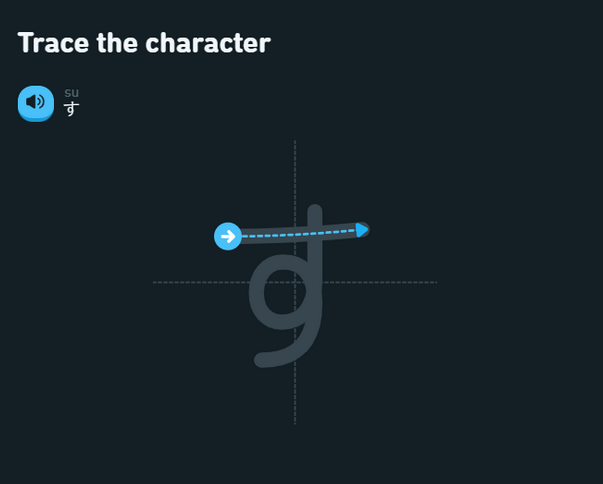
\includegraphics[width=0.5\linewidth]{resx/duolingo1.png}
    \caption{Duolingo's first type of writing exercise}    
\end{figure}

The second type is similar to the first, except the snapping feature is disabled so the task is now freehand. Figure 2 is an example of how this freehand can present some issues in how an algorithm will evaluate the accuracy of the submission.

\begin{figure}[H]
    \centering
    
\includegraphics[width=0.5\linewidth]{resx/duolingo2.png}
    \caption{User is given a false positive}  
\end{figure}

The third type has no outline and is completely freehand. Sometimes, Duolingo will give the user a “Hard” task, in which they will not be given any reference of the character and instead hear it as an outputted sound. \\

The system is very intuitive, and I had very little trouble using it. Occasionally the snapping present in the first type of exercise would cause some issues with the pen following my touch. In addition the algorithm to evaluate the user's submission is too lenient in some cases. However the app encouraged me to practice daily by sending notifications, so a user could definitely learn something in a short amount of time. \\

\begin{center}
\rule{0.5\linewidth}{0.4pt}
\end{center}
\paragraph{Write It!\\}

Another app which is used to teach users how to write a foreign script is Write It! This app is more dedicated to writing the actual script used by the language, rather than covering all aspects of the language like Duolingo does. \\

As shown in Figure 3, the app splits characters up into different sections, so the user can focus on one set at a time. This means the user has a clear indication of their progress throughout using the app. A practice section is also available in the second tab where the user can choose a specific character to focus on.

\begin{figure}[H]
    \centering
    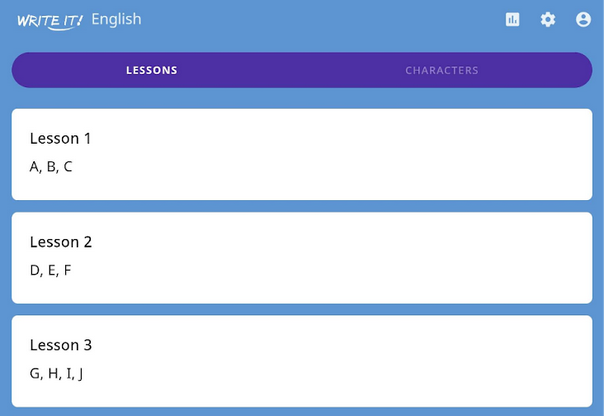
\includegraphics[width=0.5\linewidth]{resx/writeit1.png}
    \caption{Some of the available lessons in Write It!}
     
\end{figure}

The app presents two different ways of teaching the characters, similar to Duolingo. The first way is through tracing an outline of the character as seen in Figure 4. The difference between this and Duolingo is that the tracing is always freehand. However once the user has completed a stroke it automatically snaps to where it should be. \\

The second type of activity is where you cannot see the outline of the character. You are still given its shape at the top, but must draw it without the outline guide. Snapping is still enabled once the stroke has been completed.

\begin{figure}[H]
    \centering
    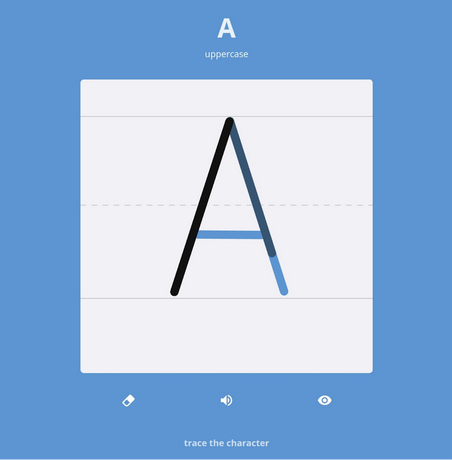
\includegraphics[width=0.5\linewidth]{resx/writeit2.png}
    \caption{Example of a writing task on Write It!}
     
\end{figure}

A major issue with this app is that it requires a particular stroke order for letters, some of which are unintuitive. This means the user must memorise the app's chosen stroke order, which is not something required to write some scripts. On the contrary, it is a simple app which anyone could figure out how to use with ease. \\

As a test for its effectiveness in learning, I downloaded the Japanese version of the app and spent a week using it. Quite quickly I noticed that it was being far too lenient with the accuracy of my strokes, similar to Duolingo. I ended up developing incorrect muscle memory because the app would correct any minor mistakes instead of marking them as wrong. In addition, I didn't find it to be helping with fluent writing, and only aided in memorising the general strokes. This may have been due to the device I was using it on: a 12.5 inch tablet. This meant I was writing the characters much larger than normal handwriting. Of course a mobile phone would provide a better scaling, but many phones do not have a touch pen, so users must use their fingers. This of course does not help in developing muscle memory when using a physical pen. However after a week I did find it had been rather effective: I was able to write every character in the Hiragana script from the sound input alone. Considering this, it would suggest the app is more useful in teaching the users the characters. Building fluency and consistency appears to not be a goal; it is instead left to the user to achieve through their own practice.

\begin{center}
\rule{0.5\linewidth}{0.4pt}
\end{center}

Both of these apps have clear indications of the user's progress, so it is important in the solution to store detailed information for each user. Furthermore both apps have a “practice mode” for studying, clearly making it a necessary feature to implement. Duolingo allows users to view the learning progress of their friends, which could improve a user's motivation to use the application. Furthermore the user interface is easy and intuitive to use, with different features of the app clearly seperated into different sections. Write It! is a much simpler application with only a few features to offer. Each `lesson' is immediately presented to the user when the app is opened, so navigation is elementary. A straight forward user interface design is therefore something that should be considered for the objectives. \\

Similarly, there is clearly an issue which the final solution should aim to not have: the leniency in evaluating the user's input. The user should not gain bad writing habits from the app, so it is important to make these mistakes clear for the user. Both applications also have many features which user's would benefit from behind a paywall, which is obviously something this project will avoid. \\

In particular, the way these applications present a user's progress in learning can be subjective. Duolingo has a section of the app in the Japanese language where each of the characters in the scripts appear with a progress bar beneath them. This does demonstrate the user's confidence with the characters, however fails to tell the user if they lose fluency---perhaps after taking a significant break from using the application. This is because the user does not receive feedback after each individual task in the lessons, so their only guide is their average progress. Therefore it is important for the user to receive immediate feedback in the technical solution.

\subsubsection{Potential Algorithms}

As the problem requires an accurate evaluation of an image, a multi-layered neural network is essential in the technical solution. Hence an algorithm to train this network will also be required. In this case where the network is classification based, the backpropagation algorithm will be most suitable. However many algorithms besides backpropagation exist, and researching these would be beneficial. \\

A database may also be necessary to store information about the user, such as username and average accuracy. This is a suitable choice as SQL queries can be used to retrieve and update data quickly. The database may also need to store a password for users, which should be hashed for security. \\

Furthermore, SignalR could be used to host a server which users can connect to. This allows for multiplayer gamemodes, and reduces processing client-side. A client would need to login with their credentials, so the database must be stored on the server for security. This also allows the neural network to be stored server-side, alleviating the client of extra processing and thereby reducing lag for lower-end devices. I have chosen to use SignalR as it can easily be used to invoke methods on both the client and server, and does not require any input from the user in order to connect. \\

If I was to implement a client-server network, object-oriented programming would be a highly suitable solution for implementing the current active games. The games could be stored in a list of their classes, providing an easy way to queue a user into a game.

\paragraph{Matrices\\}

Since this project requires a neural network, matrices must be implemeted to execute the mathemetics required by a neural network. Matrices are represented as a 2D array of numbers. They can have basic operations applied to them such as addition and multiplication, though the processes behind these operations differ from standard mathematics. Show below is an example of matrix addition and multiplication---the two operations required for a neural network: \\

\(\begin{bmatrix}
    a_1 & b_1 \\
    c_1 & d_1 \\
\end{bmatrix}
+
\begin{bmatrix}
    a_2 & b_2 \\
    c_2 & d_2 \\
\end{bmatrix}
=
\begin{bmatrix}
    a_1+a_2 & b_1+b_2 \\
    c_1+c_2 & d_1+d_2 \\
\end{bmatrix}\)

\vspace{1em}
Matrix addition is element-wise, so only works if the matrices have the same dimensions. In this case the matrices have dimensions \(2\times 2\), and add together to create a matrix of dimensions \(2\times 2\). Multiplication is not element-wise and instead sums the product of columns against rows. If a matrix \(A\) has dimensions \(a\times b\) and matrix \(B\) has dimensions \(c\times d\), only the condition \(b=c\) is sufficient for \(AB\) to be evaluated. The resulting matrix will have dimensions \(a\times d\). \\

\(\begin{bmatrix}
    a_1 & b_1 \\
    c_1 & d_1 \\
\end{bmatrix}
\cdot
\begin{bmatrix}
    a_2 & b_2 \\
    c_2 & d_2 \\
\end{bmatrix}
=
\begin{bmatrix}
    a_1\cdot a_2+b_1\cdot c_2 & a_1\cdot b_2+b_1\cdot d_2 \\
    c_1\cdot a_2+d_1\cdot c_2 & c_1\cdot b_2+d_1\cdot d_2 \\
\end{bmatrix}\)

\paragraph{Neural Network\\}

A neural network can be abstractly represented as a series of complete weighted bipartite graphs. This allows for a network to be represented a set of adjacency matrices. These are 2-way tables which store the weights between two nodes. Although these adjacency matrices are weighted, having the ability to store the absence of a connection between neurons is unneccesary since the graphs are complete. \\

The training data could be sourced from the EMNIST database: a collection of \(28\times 28\) images featuring upper and lower case latin characters. There are over 200,000 images and labels in this dataset, therefore being highly suitable for training the network. These can be stored using 2D arrays which will be converted to a 1D array to input into the network. \\

As for the forward pass in the network, it is likely that I will choose to use a library for matrix multiplication. While it is possible to build a multiplier myself, it is imperative that the forward pass is as efficient as possible. Hence I plan to use the MathNet.Numerics library. The activation function I plan to use in the hidden layers is the sigmoid function, rather than Rectified Linear Unit (ReLU). Since this is a classification network, it can be useful to retain any negative neuron values.

\begin{table}[H]
\centering
\renewcommand{\arraystretch}{1.5}
\begin{tabular}{>{\centering\arraybackslash}p{0.4\textwidth}>{\centering\arraybackslash}p{0.4\textwidth}}
\toprule
\textbf{Sigmoid} & \textbf{ReLU} \\
\midrule
\vspace{1ex}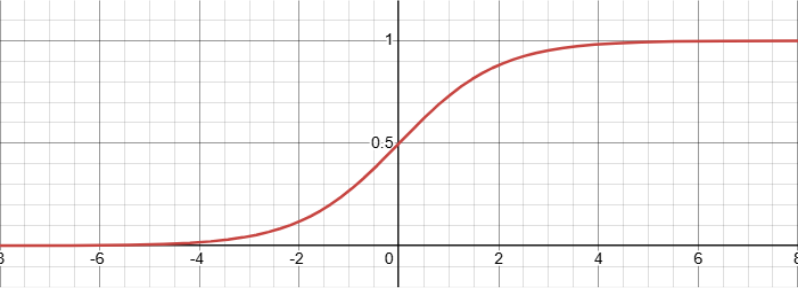
\includegraphics[width=0.35\textwidth]{resx/sigmoid.png} &
\vspace{1ex}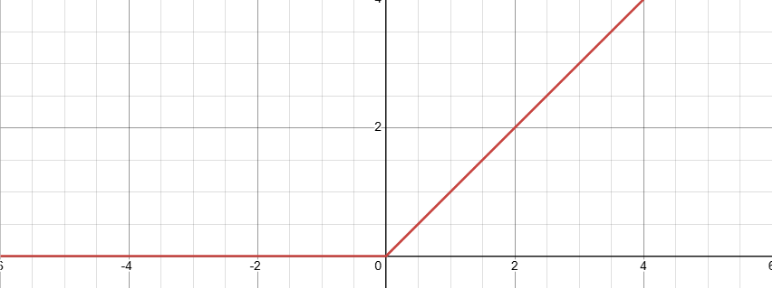
\includegraphics[width=0.35\textwidth]{resx/relu.png} \\
\bottomrule
\end{tabular}
\caption{Comparison of activation functions}
\end{table}

For the output layer I have chosen to use the softmax function rather than the sigmoid function. Softmax takes the neuron values and converts them into probabilities, such that all activated outputs sum to 1. This is far more useful in a classification network, and makes some equations faster to compute, since the derivative of the softmax function cancels out. \\

The algorithm used to train the network consists of adjusting the values of the weights and biases to reduce a “cost” function. Each neuron is given an error term, depending on how close its value is to what was expected. This allows for the weights and biases to be adjusted in such a way that the cost function is reduced. \\

The backpropagation algorithm uses calculus to minimise the cost function through gradient descent. Each parameter of the network can be represented as a dimension, such that partial derivatives can be used to minimise within the multi-dimensional space these paramaters create. The network can have thousands of these `dimensions' which is not something we can visualise. However this does not affect the mathematics behind minimising the cost function; partial derivatives are not limited to any number of dimensions. \\

Other algorithms include Contrastive Divergence which is commonly used in Boltzmann Machines. This is generally used to train energy-based models without direct backpropagation through the whole network. Instead of computing exact gradients, it defines a probability distribution over data with an energy function. The weights are adjusted such that the model assigns high probablility to training data. This method of training is more useful in correlation based problems, but is approximated so can be inaccurate for classification networks.

\subsubsection{First Interview}
\paragraph{End User\\}

Before the interview began I introduced the end user to the general concept of the solution. I informed them of how it would consist of a handwriting task which is evaluated by the app, with the aim of teaching users how to write in the English script.

\begin{enumerate}
    \item \textbf{When you were learning to write in English, do you think an app to provide instant feedback would have aided you?} \\ Yes it would have help me finding correct pronunciation \& meaning of word. most of the time you waste so much time energy in googling things.
    \begin{enumerate}
        \item \textbf{By this I mean writing in the script that English uses. Your native language uses different characters from English, so how did you learn how to write the ones used in English?} \\ so basically as you now I am from india and english is my second language but let me you fact about indian that we type hindi using english letters we do that by similar sound of character  For example :- \\ English :- what are you doing ? \\ Hindi ( using english letters) :- aap kya kar rhe hoo?
        \item \textbf{So how did you learn how to write those messages with a pen and paper? Was it taught at school for example?} \\ nope ! it just because of evolution of tech industries in india ( early 2000) becuase english is standard global language that time mostly tech ( laptop , phone ) they use english keyboard only we kinda developed  this ability. \\ that grated  goes to our kindergander teacher they hold our hand write english charactor on paper while speaking it. many practice again \& again we use to have a book which english alphabet in dot pattern \& we have to use pencil and connect all dots.
    \end{enumerate}
    \item \textbf{What statistics do you think should be measured for the user? For example, the accuracy of a submission or the time it took?} \\ Accuracy is matter more cause there is no point if you are giving wrong answer. people can buildup speed after practicing \& once they are getting right answer they will hit dopamine and it motivate them to learn english more often.
    \begin{enumerate}
        \item \textbf{So what else should be measured other than accuracy?} \\ You can measure ! How many times he try to practice his mistake and How frequently he play Quiz \& for how long
    \end{enumerate}
    \item \textbf{Do you think a multiplayer gamemode would increase how much people enjoy playing, and therefore learn faster?} \\ Yess I believe that it will help people learning fast because today generation is competitive about games they don't like to loose cause of that they will think harder \& faster.
    \begin{enumerate}
        \item \textbf{To avoid people of different fluencies being matched in an online game, do you think there should be a ranking system?} \\ Yes ranking system should be mandatory cause otherwise different fluencies will be get matched they will suffer lose in games \& some might Quite app for not being fair to them.
    \end{enumerate}
    \item \textbf{Would a “Study Mode” be beneficial to the app, which removes all competitive features and rankings---allowing users to improve at their own pace?} \\ noo I don't think so you can create different page for private space learning \& searching word and playing Quiz with engine.
    \begin{enumerate}
        \item \textbf{Just to clarify, is a private learning space a good idea?} \\ Yess
    \end{enumerate}
    \item \textbf{For more advanced users who are using the program to improve their speed, how could it be made more difficult to keep up their motivation?} \\ By teaching them new thing about their interest which don't know about it. This will tell them that they don't know everything and there is still room for learning.
    \item  \textbf{Do you think implementing localisation for common languages would benefit those less familiar with English?} \\ I feel best \& right way to learn english is that you should learn english language only because it will develop thought process in user to think in english more fast \& they will not feel english as rocket science.
    \begin{enumerate}
        \item \textbf{By localisation, I mean should a user be able to switch the text in the app to French if they are learning French instead of English? They both use the same alphabet.} \\ app function can be in english but Quiz type or learning should be in french then. It depends on what is their first language so we can understand. In which language he will understand app function?
        \item \textbf{Since they are not learning English, they will only understand French and their first language.} \\ then it should be in french
    \end{enumerate}
    \item \textbf{Would you like to see how you are improving over time, perhaps in the form of a timeline/graph of your rank?} \\ Noo I rather like to see my mistake only cause it will make me only focus on my mistake which I need to work on it.
    \begin{enumerate}
        \item \textbf{Do you think being able to view other user's graphs would aid in motivation as it adds competition between peers?} \\ Nope I believe that mine growth matter more than other person \& somehow I feel comparison is always wrong it makes people demotivated.
    \end{enumerate}
    \item \textbf{Would a gamemode where the user does not get visual feedback on their drawing be helpful? This would mean the character has to be drawn completely from muscle memory.} \\ I am not sure about this one it depends person to person so I can't say anything about this.
    \item \textbf{Would it help motivation if there was a leaderboard system in place to encourage practice?} \\ A notification reminder of doing practice will be more help than leader board system. Mostly people forget they haven't practice single time in a day \& I feel combativeness is good thing but leader board system will be too much distracting for users.
    \begin{enumerate}
        \item \textbf{If the app were to have a `friends' system implemented, would a leaderboard dedicated to showing only your friends' ranking be useful to have and why?} \\ I am against to leader board system but friends system can help user to open app more often so friend system is good idea.

        \item \textbf{How else could a user be motivated to consistently use the app?} \\ Consistency is key Success what I mean to say is that you can show them they are practice daily which make them feel proud and they will more motivated.
    \end{enumerate}
\end{enumerate}

\begin{center}
\rule{0.5\linewidth}{0.4pt}
\end{center}

Overall I felt that this interview with my end user was satisfactory. They were able to identify and suggest key features for the solution, and express concerns for elements I had at first considered suitable. While their answers could be unclear at times due to their limited fluency in English, I still believe the solution has benefitted from this interview. \\

For future interviews, I will have to consider the complexity of the language which I use. There are a few questions in which the response suggested they did not fully understand the question, such as question 6. In those cases, I reiterated the questions which I deemed were misinterpreted using simpler language.

\begin{enumerate}
    \item This question showed me how schools teach the writing aspect to the English language. They use a dot-to-dot method to allow students to gain muscle memory, repeating many times for fluency. However they said that a teacher often guides their hand, which implies teaching a whole class can take a long time. It also revealed how prevalent the English language is within modern society, such that phones use English keyboards instead of Hindi. This shows how important it is for people to be fluent in writing in English.
    \item They clearly point out a key detail here that I missed: a user can submit anything quickly to have a very low average time. I will need to find a way to counteract this based on the accuracy of a submission. \\ The suggestions for measuring frequency of each character is also a good idea, and I will consider implementing this in the database.
    \item Question 3 outlines the importance of multiplayer as a way to motivate users. Many people enjoy playing these types of competitive games, so would encourage them to learn English more often as they have stated in their response
    \begin{enumerate}
        \item They consider the possibility that without a ranking system, users could feel that it is unfair, potentially leading to them not using the app anymore. This is definitely something that should be implemented in the solution.
    \end{enumerate}
    \item They express the significance of having an offline mode where users can practise without any competitive stress. 
    \item The answer suggests they do not fully understand the aim of the solution. It could also be that they could not think of a good answer, as I could not think of anything myself either.
    \item This question makes it clear that localisation is something I will need to consider for the solution. The Latin script is used for many European languages, so the app could be used by people learning any of these languages.
    \item Another instance of a misunderstanding, however it is vaguely clear what they are intending to express. They recognise that focusing on their mistakes will help them improve faster, and hence express a desire to view their mistakes. This is not applicable to a timeline of a statistic, but does suggest a need to provide separate accuracies for the letters. This allows for displaying to the user which characters they are less confident in, allowing them to focus on these in particular.
    \begin{enumerate}
        \item They express concerns over demotivation from seeing the statistics of others who are more fluent. I will take this opinion into consideration, along with the insight of a frequent user of Duolingo.
    \end{enumerate}
    \item Not a useful answer, but possibly could have been too confusing of a question.
    \item In this question they consider how a leaderboard could be ineffective for motivation. They state how a daily notification or reminder could encourage users to practise daily, so this is something that should be present in the solution.
    \begin{enumerate}
        \item This question makes it clear how peer pressure could be used passively to motivate users to practice their writing skills. If a user were to see their friends doing better than them, it could encourage them to try and improve themselves.
        \item They suggest implementing something which tracks how many days in a row someone has used the app. This is a feature present in Duolingo known as a `Daily Streak'. It acts as motivation since users will try to not `lose' their streak. However this is also utilised in many free mobile games with malevolent intention---more time spent using the game will increase revenue for the developers. In some cases their `encouragement' for a user to play everyday can turn into an addiction, which is something I intend to avoid. Hence I will not be implementing a Daily Streak into the final solution.
    \end{enumerate}
\end{enumerate}

\begin{center}
\rule{0.5\linewidth}{0.4pt}
\end{center}

\paragraph{Duolingo User\\}
I have also chosen to interview a frequent user of Duolingo, as referenced in Objective 1.4.1. Duolingo has been active for over 10 years and has over 500 million downloads, so it would be beneficial to understand what makes this app effective.

\begin{enumerate}
    \item \textbf{Considering you are an active user of Duolingo, what features encourage you to commit to learning a new language, and why?} \\ The idea of having a streak, meaning you would be very sad if you lost it. Having friends as well, with friend streaks, so there actually is something to lose if you don't do your duolingo. The app also has a very nice UI that is really intuitive and appeals to me, with great haptic feedback too. The way you learn is also great, with duolingo sometimes revisiting past topics for memory recall. Lastly, the idea of having levels so you can enumerate where you are in terms of progress.
    \item \textbf{How important is it for the user to have a clear indication of their progress?} \\ Very important. Like I said before, having a way to check your progress means you are less likely to get lost and just give up. It is also fun to see the change in progress over time.
    \item \textbf{Would you say Duolingo's UI is relatively easy to navigate? How important is this for a language learning app?} \\ It is easy to navigate. It looks beautiful, clean and simple, with vibrant colours that appeal to most young people like me. Of course this is important: If it was convoluted or hard to use or not enticing, you risk driving away a lot of users who may care about it like me.
    \item \textbf{If Duolingo had online multiplayer where you could learn with your friends, would this compel you to use the app more frequently?} \\ Yes. Duolingo already has the idea of friend streaks, and a graph that shows how much XP you have gained over the week vs how much the other person has upon clicking on their profile. This is a great feature to have to enable especially competitive people to make lots of progress together.
\end{enumerate}

From this response it's clear that Duolingo utilises many ways to keep its users engaged and active with learning. The interviewee expresses how the friends system can be motivating, implying that it compels them to consistently use the app. Adding a daily streak which records how many consecutive days you have opened the app, and a levelling system appears to be something I should take into consideration. It is clear that a way to store statistics about a user's performance is necessary in the solution. I should also consider the UI design, as the app language will be in the language that the user is learning. It is therefore important to utilise icons as well as text to convey what each element of the application does.

\subsubsection{Key Requirements}

After completing my research and interviews I have determined that one of the key
requirements is an SQL database to store statistics regarding a user's progress. Detailed information on a user's progress for different characters is something that must be present in the final solution. \\

Furthermore a client-server network is essential in securely storing a user's data, since accounts are also a necessary requirement for this project. A multi-layered classification neural network is also a key requirement as the program must be able to evaluate an image. Linking to this, a way of the user to input this drawing in an intuitive and easy manner is also vital. \\

Concerning features of the app rather than core functionality, a way to rank users based on their skill is also very important. The app should also encourage users to use it consistently, since developing muscle memory requires persistent effort from those learning. However this should not be done in a way that could be stressful to the user due to them potentially missing out or losing something. The motivation should be completely passive and not impact the user negatively in any way. \\

\newpage
\subsection{Further Research}

\subsubsection{Prototype}

Regarding the prototype, I decided to create the neural network and the user input. These make up the core requirement for my program, and are essential for the final solution. I anticipated that the neural network was likely to be the most time consuming part of the project, so prototyping it first was a suitable choice. While I had some experience with neural networks, I had only ever programmed an image classification for digits \(0-9\). Expanding this to have more than double the output neurons required several iterations of testing, since it was unclear what an optimal structure for the network would be. \\

While programming the network, I kept in mind how the solution would use Object-Oriented Programming. It was important to use classes appropriately to allow me to seamlessly integrate it into the techincal solution. After programming a beta for the network, I sourced the training data and attempted to train the network. There were several bugs at first where I had implemented the equations incorrectly. \\

After patching all of the bugs, I began the train the network but noted it was rather slow. Looking into the process, I noted that the network parameters were reloaded from their files for each iteration. This is inefficient since the parameters will only be updated after every batch of 50 images. I had originally coded the class that performs the forward pass to load the parameters every time, since this would be optimal while evaluating real data. However in training, the parameters only need to be reloaded every 50 images, so I added a second constructor which takes in the weights and biases as parameters. This dramatically sped up the training process, allowing me to identify if it was working much faster. \\ 

Initially I attempted to train the network with a \(784-192-144-52-26\) structure, however it quickly became apparent that the weight gradients started to vanish or explode after enough training data. This is where the weight values tend to either zero or infinity, which leads to the model under/overfitting. After some research into layers, I deduced that the network should have at most 4 layers to prevent these issues. Eventually I settled on a \(784-144-72-26\) structure, which achieved 94\% accuracy with the training data.

\paragraph{Execution\\}
Upon running the prototype, the user is presented with a Windows Form containing a read-only textbox and a panel for input. They are given 10 successive characters in the textbox and are tasked with writing them in the panel using mouse input. \\

The user can then click “done” once they have finished writing, and the image is evaluated by the neural network which returns the letter written by the user.

\vspace{1em}
\begin{figure}[H]
    \centering
    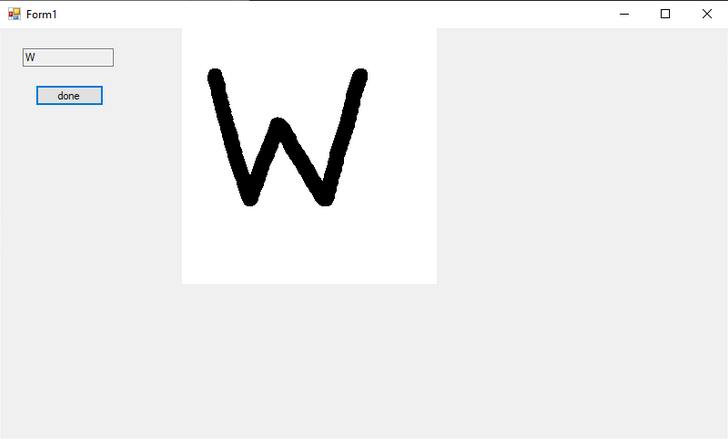
\includegraphics[width=0.5\linewidth]{resx/prototype.png}
    \caption{The user is able to draw on the panel}
\end{figure}

\paragraph{Function\\}
The panel uses the System.Drawing.Pen class in order to draw on the panel. The input contains a method enablePanel() which attaches event handlers to mouse movements and clicks. When the mouse is moved, the mouseMoved() event handler is called, which will draw a line connecting the last mouse position to the new mouse position if the left mouse button is pressed. The last mouse position is then updated for the next mouse move event, regardless of whether the left mouse button was pressed. \\

When the user clicks “done”, the event handlers for drawing on the panel are removed, and the image drawn on the panel is saved as a Bitmap type. This bitmap is then downscaled to \(28\times 28\) in size to match the input layer of the neural network. Each pixel has a red, green, and blue value. The image is converted into grayscale using the formula for luminance:

\begin{equation*}
    L = 0.299 R + 0.587 G + 0.114 B
\end{equation*}

While the original image is only white and black, the downscaled Bitmap will introduce grey tones, which are represented in RGB format. The formula allows the program to convert these RGB values into a grayscale brightness with a value ranging from 0 to 255. Each of these values is then divided by 255 to obtain a value representing the brightness from 0 to 1. These values are then assigned into a 784 length array and fed into the input layer of the neural network. The output activation values are then calculated as described in Objective 1.4.2.1. The result is then outputted to the user for them to judge their accuracy.

\paragraph{Analysis\\}
I noted during testing that the input had to be centered and the right size for an accurate evaluation. This suggests that the images need to be preprocessed in order for the neural network to function properly. I also found that the size of the pen had a significant effect---it is likely the optimal pen size is one that most closely matches the training data. \\

UI design is an aspect which was not considered when creating the prototype, as the goal of it was to see if the algorithms chosen were a viable option for the final solution. Since the neural network has been successfully implemented, it is appropriate to implement the prototype into the technical solution. The prototype has shown that the solution is feasible in the time given.

\subsubsection{Second Interview}
\begin{enumerate}
    \item \textbf{After familiarising yourself with the draft objectives, are there any features missing that you expected to be present?} \\
    If there is a password system, perhaps add a way for the user to change the password. \\
    If there is a friends system, it might be useful for there to be an invite system.
    \item \textbf{Regarding the prototype, would you say the program is accurately evaluating your input?} \\ 
    Fairly accurate, but it requires the letter to be written in a very specific way towards the centre of the box, which is fairly annoying. Some letters seem more accurate than others.
    \item \textbf{Would you say the input method is easy to use?} \\
    Yes. Drawing seems very responsive, although drawing with a mouse is quite different to drawing with a pen, and it feels a little less controlled.
    \item \textbf{In what ways would you like the UI to be improved in the final solution?} \\
    Make the written letter disappear before the next one can be written. \\
    Make the UI scale when the window size is changed. \\
    Add undo or clear buttons.
\end{enumerate}

\begin{center}
\rule{0.5\linewidth}{0.4pt}
\end{center}

Overall this interview didn't provide me with significant information I was unaware of, but there are some key points worth highlighting. The majority of the comments were issues I had found myself while using the prototype, such as the drawing panel not being cleared. \\

However the interviewee also suggested to implement a `clear' button for the panel, something I will consider for the technical solution as it improves user experience. Furthermore they identified some missing objectives which may be useful in the project, such as a system to add other users as a friend. It is also clear from the response that I will need to implement preprocessing for the images, since the neural network can only evaluated images drawn to a similar scale and size as the EMNIST dataset. I will also investigate why some letters are more accurate than others but I suspect this is due to certain Latin characters being similar shapes. \\

The issue of mouse input is not something I can easily fix, and does rely on a user having a drawing tablet if they wish to gain correct muscle memory. While I was testing the prototype myself I noticed that it did not encourage memorisation in its current state and purely focused on muscle memory. This is due to the character being on display at all times while the user is submitting their drawing. It may be suitable to add options to the technical solution which only show the character for a few seconds. However this raises some issues if the user were to miss its appearance, so perhaps focusing on elementary writing skills is a better option. Even a user passively copying what they see on screen will eventually develop their muscle memory to a sufficient state.

\newpage
\subsection{Objectives}
The objective of this program is to allow users to practice writing the Latin script. The user has the option from three different gamemodes, and they have statistics detailing their progression in learning each of the Latin characters. The user interactes with the project through the client application, which establishes a connection to the server application. The server manages the progression of the different gamemodes, and stores a user's account data and statistics.

\subsubsection{Core Objectives}
\begin{enumerate}
    \item {\textbf{Accounts}}
    \begin{enumerate}
        \item The user will be able to enter their account credentials and login.
        \begin{enumerate}
            \item If the entered username does not exist, or the password is incorrect then access will be denied.
            \item Otherwise the login screen will close and the main app will open.
        \end{enumerate}
        \item The user will be able to request an account creation.
        \begin{enumerate}
            \item If any fields are left blank, or the passwords do not match then the account creation request is not sent.
            \item If the entered username is already in use then the account cannot be created.
            \item Otherwise a new account will be created in the database and the main app will open.
        \end{enumerate}
        \item There will be a button to cycle through languages on the login screen, which will affect the language associated with the account upon account creation.
    \end{enumerate}

    \item \textbf{Games}
    \begin{enumerate}
        \item A game will start when it has the maximum number of users queued for it.
        \item The user will be presented with successive, randomly generated Latin characters.
        \item The user will be able to use mouse input to write the character in a blank panel.
        \begin{enumerate}
            \item The user will be able to clear the panel of any drawings.
        \end{enumerate}
        \item The user will then receive feedback on the accuracy and time of their submission.
        \item \begin{enumerate}
            \item The accuracy and elapsed time will contribute to the averages stored in the database.
        \end{enumerate}
        \item A list of all of the users in a game will be displayed to the users, and is updated when a user joins or leaves.
        \item An overview of the statistics for the previous rounds will be displayed.
        \item The next round of each game will start when all of the users are ready.
        \item There will be three different types of games to choose from:
        \begin{enumerate}
            \item \textbf{An offline game for practicing}
            \begin{enumerate}
                \item The game will consist of 10 rounds, each with a randomly generated Latin character.
                \item After each round the user will be given their time and accuracy, and their statistics for the completed rounds will be shown during the game.
            \end{enumerate}
            \item \textbf{A Versus game}
            \begin{enumerate}
                \item The user's performance will affect their rank, which is recalculated after the end of every game.
                \item After each round, the user with the fastest time will win the round. If one player is incorrect then the other player will be given the win. If both players are incorrect then neither of them win.
                \item After each round the users will be given their time and accuracy, and the user who won the round will be displayed.
            \end{enumerate}
            \item \textbf{An elimination game of 12 users}
            \begin{enumerate}
                \item After each round the users who are incorrect will be eliminated  and given the option to return to home. If all of the submissions are correct then the user with the longest time will be eliminated instead. If none are correct then no user will be eliminated.
                \item After each round the users will be given their time and accuracy, and the list of alive and eliminated users will be updated.
                \item The last user remaining is the winner and the game will end when this occurs.
                \item The next round of the game will start when all of the alive users are ready, and will ignore any eliminated users.
            \end{enumerate}
        \end{enumerate}
    \end{enumerate}    

    \item \textbf{Statistics}
    \begin{enumerate}
        \item There will be a `profile' page which displays detailed information about a user.
        \begin{enumerate}
            \item The statistics for each letter will be displayed, which includes the average accuracy, average time, and total attempts.
        \end{enumerate}
        \item The statistics for each user will be separated by letter in the database, 
        \item A user's rank will have a rank to quantify their confidence writing the Latin characters.
        \begin{enumerate}
            \item The rank will be recalculated following a `Versus' game using the Elo formulae.
        \end{enumerate}
        \item A user can view the profile page of any other user through an exact-match search tool.
    \end{enumerate}

    \item \textbf{Social}
    \begin{enumerate}
        \item There will be an option to add/remove friends on their profile page.
        \begin{enumerate}
            \item An invite will be forwarded to a user if they are online, otherwise it will be stored in a database.
        \end{enumerate}
        \item A user's friends will be listed in the main menu.
        \begin{enumerate}
            \item They will be separated into `online' and `offline'.
            \item A user can open their friend's profile page from this menu.
        \end{enumerate}
        \item A user can choose from various language which use the Latin script for the client application to use.
        \begin{enumerate}
            \item The language chosen by the user is saved in the database.
            \item The user can update the language of the application.
        \end{enumerate}
    \end{enumerate}

    \item \textbf{Server}
    \begin{enumerate}
        \item A user will be able to connect to the server from any device running the client application.
        \item The server should manage the progression of currently active games.
        \begin{enumerate}
            \item The server should initiate each phase of the game when the conditions for it are met, and start and end each game as required.
            \item When a user queues for a game, the server should appropriately assign the user to a game.
        \end{enumerate}
        \item The server will utilise a multilayered neural network to evaluate the accuracy of a submission.
        \begin{enumerate}
            \item A user's submission will be preprocessed to match the formatting of the training data.
            \item The network will accurately classify a user's submission into one of the 26 Latin characters.
            \item The user will be able to draw their submission to any size and scale.
        \end{enumerate}
        \item The server will store a database containing data for each registered user.
        \begin{enumerate}
            \item For each user, the database will store their password, account details, and statistics.
            \item Passwords in the database will be hashed.
        \end{enumerate}
    \end{enumerate}
    

\end{enumerate}

\subsubsection{Extension Objectives}
\begin{enumerate}
    \item If a friend is online, the user can invite them to a Versus game.
    \item A user can create a private game which requires invites to join.
    \item The user's rank over the last 90 days will be stored to allow a timeline graph to be produced.
    \item There will be an option to disable visual feedback for the input.
\end{enumerate}

\newpage
\subsection{Modelling}
\subsubsection{Class Diagrams}
I will be using Object Oriented Programming (OOP) in this project, so class diagrams are an essential part of the modelling phase. I have produced class diagrams for the both the client-side and server-side projects to assist with coding the technical solution. These are not final, and will likely be changed during Design.
\begin{figure}[H]
    \centering
    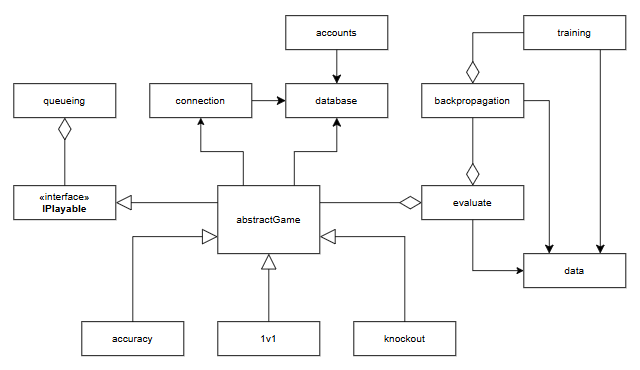
\includegraphics[width=0.75\linewidth]{resx/server_class_1.png}
    \caption{Server class diagram}
\end{figure}
\begin{figure}[H]
    \centering
    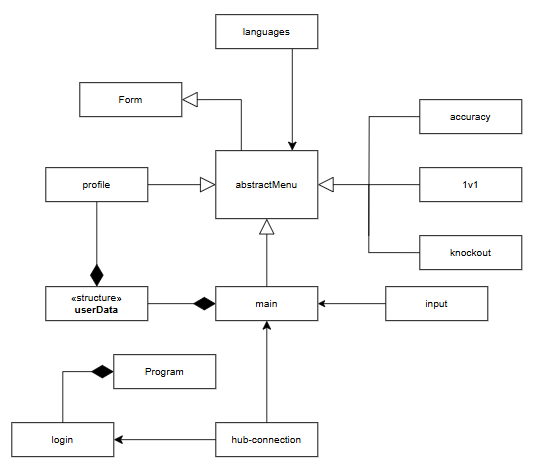
\includegraphics[width=0.7\linewidth]{resx/client_class_1.png}
    \caption{Client class diagram}
\end{figure}
\subsubsection{Flowcharts}

The below flowchart describes the abstracted login/account creation process for a client. The user is presented with the option of creating an account or logging into an existing one. In each case, several checks are done using the database before loading the main application. For logging in, the server must first ensure that the account exists, and then checks if the passwords match. For creating an account, the server must check if the username entered is already in use. If the entered information is valid, the client is sent their user data and any pending invites.

\begin{figure}[H]
    \centering
    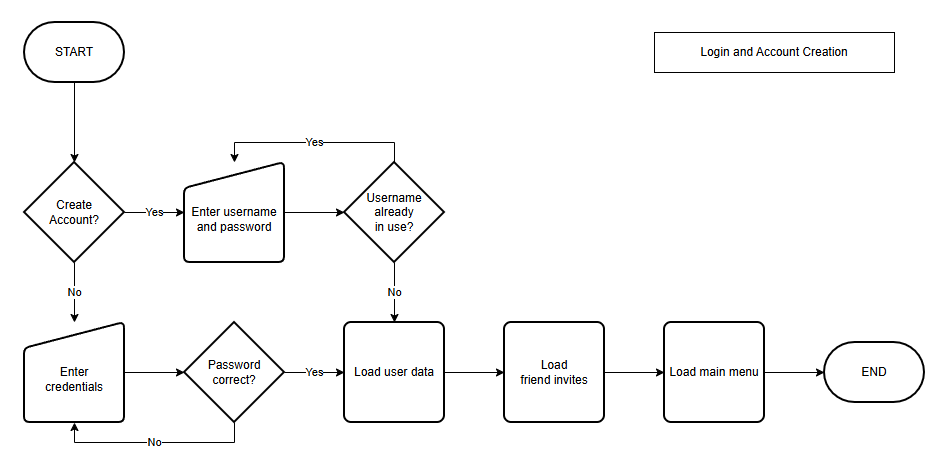
\includegraphics[width=1\linewidth]{resx/flow_login.png}
    \caption{Account flowchart}
\end{figure}

The following flowcharts provide an abstract representation of how each game type will operate. The details of each game type can be found in Objective 1.6. When a user queues a certain game, the server checks if there is space for the user to join. If the lobby then becomes full, the game starts.

\begin{figure}[H]
    \centering
    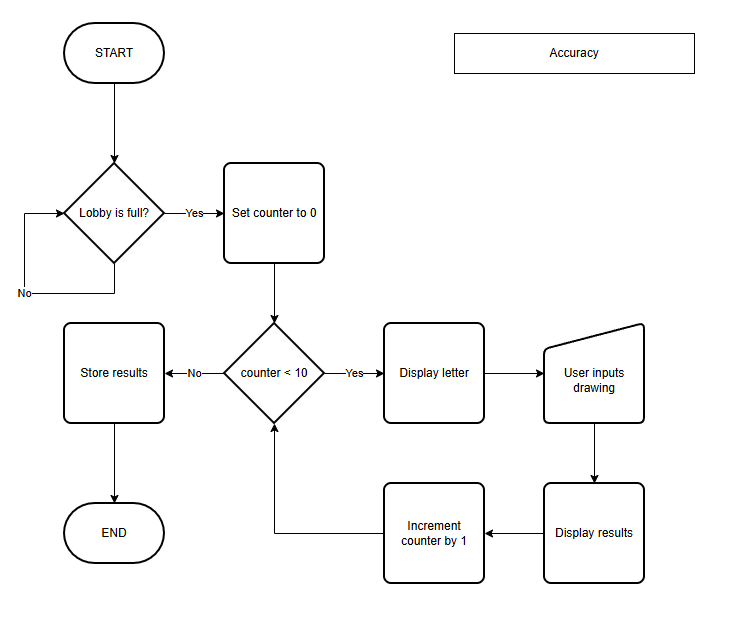
\includegraphics[width=0.75\linewidth]{resx/flow_accuracy.png}
    \caption{Accuracy flowchart} 
\end{figure}
\begin{figure}[H]
    \centering
    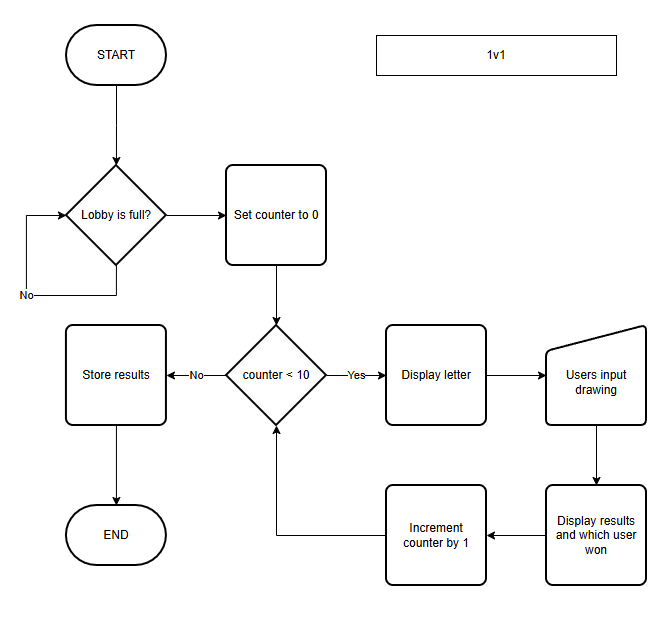
\includegraphics[width=0.64\linewidth]{resx/flow_versus.png}
    \caption{Versus flowchart} 
\end{figure}
\begin{figure}[H]
    \centering
    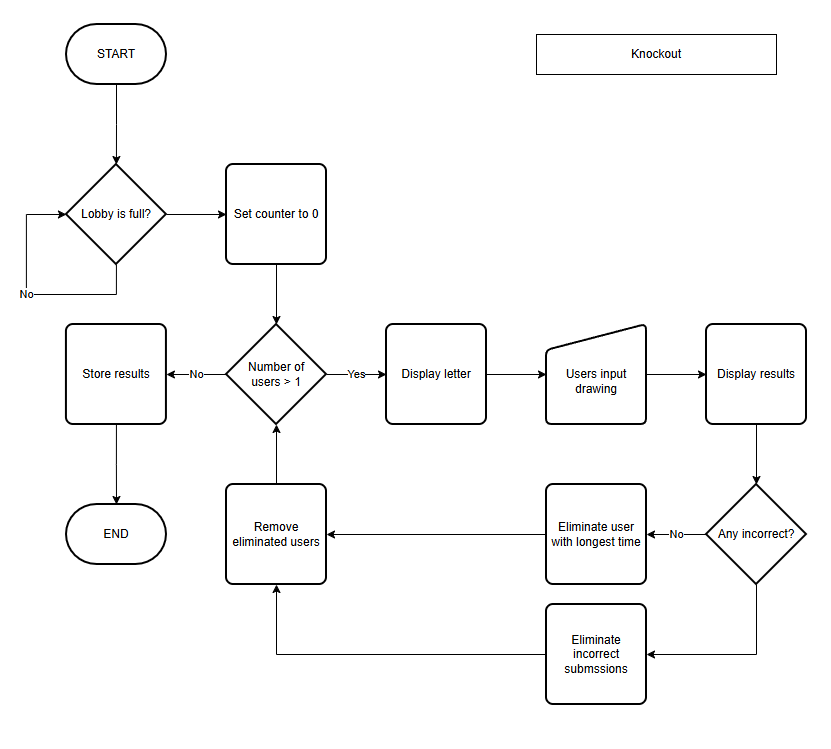
\includegraphics[width=0.75\linewidth]{resx/flow_knockout.png}
    \caption{Knockout flowchart} 
\end{figure}

\subsubsection{Entity-Relationship Diagram}
The following is an entity-relationship diagram. The \textit{userData} table holds information regarding each user with an account. Each user has a unique identifier which is stored in \textit{userID}, along with a password for their account. The table also stores a user's rank, and their preferred language. I have also added an `about me', where users can write something about themselves if they wish. This table is linked to the \textit{statistics} table which contains a user's progress for each Latin character.

\begin{figure}[H]
    \centering
    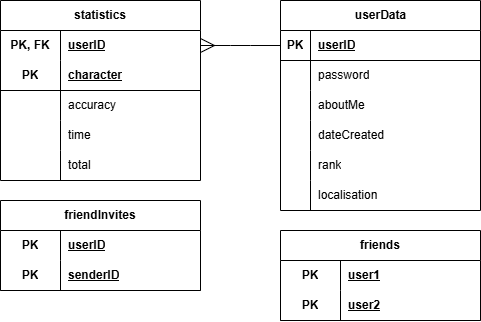
\includegraphics[width=0.5\linewidth]{resx/sql.png}
    \caption{Entity-Relationship diagram} 
\end{figure}

The \textit{statistics} table details their average accuracy and average time, along with the total number of times the user has completed the character. This allows the averages to be updated by using the following formula:

\begin{equation*}
    A_{new}=\frac{A_{current}\cdot \text{total}+ \text{accuracy}}{\text{total}+1}
\end{equation*}

Since friend invites can be sent while the receiving user is not online, it is necessary to cache the invite for when the user next logs on. This is done using the \textit{friendInvites} table. Friendships exist using the \textit{friends} table---only one link exists for each friendship.

\subsubsection{Neural Network}
A neural network consists of several complete weighted bipartite graphs. The first layer is referred to as the input layer, and the final layer is referred to as the output layer. The layers in between are referred to as the hidden layers, as shown in the figure below.

\begin{figure}[H]
    \centering
    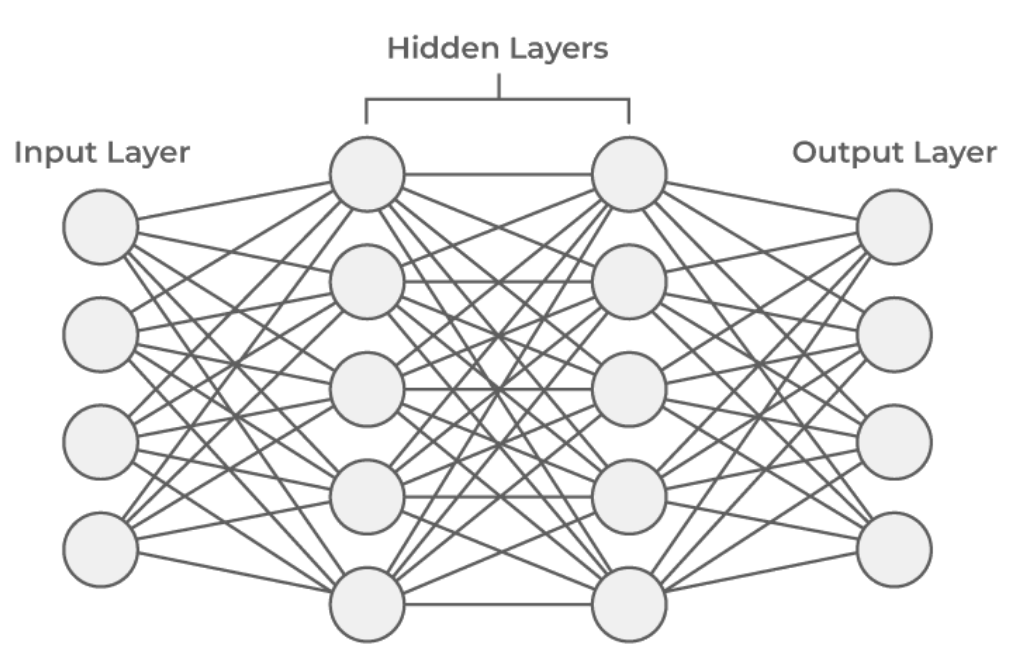
\includegraphics[width=0.5\linewidth]{resx/network.png}
    \caption{Simplified version of a neural network}
\end{figure}

Each layer consists of a set number of `neurons' which each hold a decimal value. The arcs connecting a neuron to all the neurons in the next layer also hold a decimal value, referred to as a `weight'. All the neurons, except those in the input layer also have a fixed `bias'. An activation function is also used to normalise the neuron values. As outlined in Objective 1.4.2.1 this will be the sigmoid function for the hidden layers, and the softmax function for the output layer. \\

\noindent The notations used to denote neural networks is outlined below:
\vspace{1em}

\begin{align*}
  z_{i}^{(L)} &\longrightarrow \text{the value stored in the } i^{\text{th}} \text{ neuron in the } L^{\text{th}} \text{ layer} \\
  a_{i}^{(L)} &\longrightarrow \text{the activated value stored in the } i^{\text{th}} \text{ neuron in the } L^{\text{th}} \text{ layer} \\
  w_{i,j}^{(L)} &\longrightarrow \text{the weight on the arc from the } i^{\text{th}} \text{ neuron in layer } L \text{ to the } j^{\text{th}} \text{ neuron in layer } L+1 \\
  b_{i}^{(L)} &\longrightarrow \text{the bias of the } i^{\text{th}} \text{ neuron in the } L^{\text{th}} \text{ layer} \\
  \delta_{i}^{(L)} &\longrightarrow \text{the error value of the } i^{\text{th}} \text{ neuron in the } L^{\text{th}} \text{ layer}
\end{align*}

\vspace{1em}

\begin{center}
\rule{0.5\linewidth}{0.4pt}
\end{center}
\paragraph{Forward Propagation\\}
Forward propagation is the process by which values are placed into the input layer of the network, and a set of values is produced in the output layer. Each neuron in a layer is calculated using the values stored in the previous layer's neurons, using the following formula, where \(n(L)\) is the number of neurons in the \(L^\text{th}\) layer:

\begin{equation*}
    z_j^{(L+1)}=\sum_{i=1}^{n(L)}{\left(w_{i,\ j}^{(L)}\cdot a_{i}^{(L)}\right)}+b_{j}^{(L)}
\end{equation*}

For each neuron in the previous layer which connects to the neuron being calculated, its activated value is multiplied by the weight connecting them. These values are then summed, and a bias is added to this result. The formula can be represented as a series of matrix operations when considering the entire layer: \\

\(\begin{bmatrix}
    w_{1,\ 1}^{(L)} & w_{1,\ 2}^{(L)} & w_{1,\ 3}^{(L)} & \cdots & w_{1,\ n(L+1)}^{(L)} \\
    w_{2,\ 1}^{(L)} & w_{2,\ 2}^{(L)} & w_{2,\ 3}^{(L)} & \cdots & w_{2,\ n(L+1)}^{(L)} \\
    w_{3,\ 1}^{(L)} & w_{3,\ 2}^{(L)} & w_{3,\ 3}^{(L)} & \cdots & w_{3,\ n(L+1)}^{(L)} \\
    \vdots & \vdots & \vdots & \ddots & \vdots \\
    w_{n(L),\ 1}^{(L)} & w_{n(L),\ 2}^{(L)} & w_{n(L),\ 3}^{(L)} & \cdots & w_{n(L),\ n(L+1)}^{(L)} \\
\end{bmatrix}
\cdot
\begin{bmatrix}
    a_1^{(L)} \\
    a_2^{(L)} \\
    a_3^{(L)} \\
    \vdots \\
    a_{n(L)}^{(L)} \\
\end{bmatrix}
+
\begin{bmatrix}
    b_1^{(L+1)} \\
    b_2^{(L+1)} \\
    b_3^{(L+1)} \\
    \vdots \\
    b_{n(L+1)}^{(L+1)} \\
\end{bmatrix}
=
\begin{bmatrix}
    z_1^{(L+1)} \\
    z_2^{(L+1)} \\
    z_3^{(L+1)} \\
    \vdots \\
    z_{n(L+1)}^{(L+1)} \\
\end{bmatrix}\)

\vspace{1em}
This results in a vector column representing the values stored by the neurons in the layer. The activation function is then applied to the layer, which for the hidden layers is the sigmoid function:

\begin{equation*}
    \sigma(x)=\frac{1}{1+e^{-x}}
\end{equation*}

For the output layer, the softmax function is used as the activation function. The softmax function converts the neuron outputs into probabilities that sum to 1, which produces a more useful output for a classification network. The output with the highest probability is the index of the letter chosen by the network.

\begin{equation*}
    \text{softmax}(x_i)=\frac{e^{x_i}}{\sum_{j=1}^{n(L)}e^{x_j}}
\end{equation*}

\begin{center}
\rule{0.5\linewidth}{0.4pt}
\end{center}
\paragraph{Backpropagation\\}
Backpropagation is the algorithm used to train a neural network. A network can be considered suitably trained when a `cost function' has been minimised. The cost function is a value that represents how far off the output is from expected. For example, if the network was given an image of the letter K, then the perfect output would be 1 in the 11th neuron and 0 in all the others. If the network does not achieve this, then the cost function will measure how far off the output was from expected. \\

The cost function I will be using is mean squared error. This is calculated by squaring the difference between the observed output and the expected output of each neuron.

\begin{equation*}
    C_i=\left(a_i^{(L)}-y\right)^{2}
\end{equation*}

To minimise the cost function, the values of the weights and biases can be changed. Backpropagation attempts to find the optimal values for these parameters by using a process called gradient descent. In summary, gradient descent uses derivatives to find the fastest way to minimise the cost function with respect to the parameters. \\

The first stage of backpropagation is to calculate the neuron errors for the output layer. This is equal to the partial derivative of the cost with respect to the weights:

\begin{equation*}
    \frac{\partial C}{\partial w^{(L)}}=\frac{\partial z}{\partial w^{(L)}}\frac{\partial a}{\partial z^{(L)}}\frac{\partial C}{\partial a^{(L)}}
\end{equation*}

Since the softmax activation function is in use along with mean squared error, this equation simplifies down to the derivative of the cost function. The value of \(y\) takes either 1 or 0, depending on whether the current neuron's index is equal to the expected result.

\begin{equation*}
    \delta_i^{(L)}=2(a^{(L)}-y)
\end{equation*}

The second stage of backpropagation is to calculate the neuron errors for the hidden layers, using the same partial derivative as the output layer. The differential equation evaluates differently in the hidden layers: the errors for a given layer \(L\) are calculated using the errors for the \(L+1\) layer, hence the name `backpropagation'.

\begin{equation*}
    \delta_i^{(L)}=\sigma'(z_i^{(L)})\cdot \sum_{j=1}^{n(L+1)}\left({w_{i,\ j}^{(L)}\cdot \delta_j^{(L+1)}}\right  )
\end{equation*}

\begin{equation*}
    \sigma'(x)=\sigma(x)\cdot (1-\sigma(x))
\end{equation*}

The error term of the \(L+1\) layer is affected by the activation function used and the weights connecting it to the \(L\) layer. The equation propagates the errors of the output layer through the rest of the network, excluding the input layer. \\

The third stage of backpropagation is to calculate the weight gradients. These represent the optimal adjustments to the weights to minimise the cost function. They are calculated by multiplying the neuron error of the \(L+1\) layer by the activated value of the \(L\) layer. The bias gradients are equal to the neuron errors.

\begin{equation*}
    \frac{\partial C}{\partial w_{i,\ j}^{(L)}}=\delta_j^{(L+1)}\cdot a_i^{(L)}
\end{equation*}

These parameter gradients are then averaged over several training iterations. A training iteration involves giving the network an image and a label, which allows it to compute the cost function. The averaged gradients are then multiplied by the `learning rate'---a value usually around 0.01 which ensures the model does not learn too fast and overfit. This average gradient is then subtracted from the current parameter to give its updated value, which is saved in a file.

\begin{center}
\rule{0.5\linewidth}{0.4pt}
\end{center}
\paragraph{Training\\}

The training data I will use is from the EMNIST database. The sample contains over 200,000 images and labels of both uppercase and lowercase Latin characters. It is stored in two GZIP files, one for the images and one for the labels. These files are formatted as byte arrays, and contain headers which are of length 16 bytes for the images and 8 bytes for the labels. The values range from 0 to 255, so they are divided by 255 before being used for training, since the neural network can only use values between 0 and 1. \\

Before a neural network can be trained, the parameters of the network must be initialised to a value. The biases can be set to zero, however doing this for the weights will cause the gradients to vanish. To avoid this issue, Xavier initialisation can be used, which assigns each weight a value taken from a uniform distribution between a limit and its negative value. This limit is calculated using the size of the layers which the weight connects together.

\begin{equation*}
    \text{limit}=\sqrt{\frac{6}{n(L)+n(L+1)}}
\end{equation*}

\begin{center}
\rule{0.5\linewidth}{0.4pt}
\end{center}

\paragraph{Image Preprocessing\\}

A submitted image is likely to not be consistent with the EMNIST dataset, therefore proprocessing is required so an accurate evaluation can be made. This was made clear in the prototype, which does not have preprocessing. Firstly, the Region of Interest (ROI) is extracted from the drawn image, which involves cropping the image into a rectangle where there is no white space surrounding the ROI.\@ \\

This rectangular crop then needs to be adjusted such that it is a square. This is done by adding white space to the shorter of the two dimensions. If the image was expanded in the Y direction, then the ROI is shifted down in order to recentre it. Similarly if the image was expanded in the X direction then the ROI is shifted right. \\

The image is then scaled to \(24\times 24\), which differs from the prototype. This is to match the dataset, which has padding on the images. The remaining pixels to create the \(28\times 28\) image are added on all sides as white space. The image is then inverted, and converted to a set of decimal values using the luminance formula, as described in 1.5.1.

\subsubsection{Client-Server Connection}

SignalR is a dotnet package used to establish a client-server connection between two devices. When the server is configured, the application maps endpoints to a class which inherits the \textbf{Hub} class. An endpoint takes the form of \textit{http://86.11.15.228:5252/cs-nea/accounts}, and will forward all invokations received by the client to the designated class. \\

The SignalR library contains methods for invoking methods on the server, which can return a value. The client will pass the method name as a string, along with any parameters, using the HubConnection type.

\begin{minted}{csharp}
    await hubconnection.InvokeAsync("requestedMethod", parameter1, parameter2);
\end{minted}

The server can invoke an action on the client using its Context.ConnectionID, a unique string which identifies a client connected to the server. This is not fixed for each IP address and is randomly generated when a connection is established. A client can set up handles to receive any packages sent by the server which are executed as an action.

\begin{minted}{csharp}
    await Clients.Client(connectionID).SendAsync("requestedAction", parameter1, parameter2);
    
    hubconnection.On<string, int>("requestedAction", (text, num) =>
    {
       Console.WriteLine("Received string: `` + text);
       total += num;
    });
\end{minted}

The identifier `requestedAction' must be identical on both the client and server to allow the request to be received. These handles are added after a connection is established, but before it is started.

\subsubsection{Player Ranking}

As discussed, it would be unfair to match players against those with a significantly different skill level. Therefore it is necessary to implement a system which can abstract a user's skill to a single number. The most commonly used rating system is the Elo rating system. \\

The Elo rating system is most famously used in Chess, but is also implemented for other competitive games. In pool, an Elo-based system called Fargo Rate is used to rank players in organised amateur and professional competitions. In both cases they use the Elo formulae to accurately rank a player's skill. \\

For a player's Elo to change, they must play in a multiplayer gamemode, usually against a single person. The system uses their expected `score' and their actual score to accurately adjust their rating. The difference in the player's ratings is used to calculate their expected scores for a given game. If player A has a rating of \(R_A\) and player B a rating of \(R_B\), the formula for the expected score of player A is 

\begin{equation*}
    E_A=\frac{1}{1+10^{(R_B-R_A)\ /\ 400}}
\end{equation*}

where \(400\) is the base rating for a player. A win is given a score of 1 and a loss is given a score of 0. Draws would be given 0.5 points which occur when all players are incorrect. The expected score for player B can be calculated as \(1-E_A\). In the case of the Versus game type, we multiply the expected score by 10 since there are 10 rounds per game. \\

When a user's actual score from a Versus game exceeds their expected score, the Elo system takes this as evidence that the user's rating is lower than it should be. This is done through a linear adjustment using the K-factor, which is the maximum possible adjustment per game. In this case where a player could theoretically score 10 points more than expected, the K-factor will be divided by 10 to ensure it remains the maximum possible adjustment. \\

\(\begin{aligned}
    K=32&\longrightarrow \text{used for players below 2100 elo} \\
    K=24&\longrightarrow \text{used for players between 2100 and 2400 elo} \\
    K=16&\longrightarrow \text{used for players above 2400 elo} \\
\end{aligned}\)
\vspace{1em}

The player's rating can then be updated with the following formula, where player A was expected to score \(E_A\) points but actually scored \(S_A\) points:

\begin{equation*}
    R'_A=R_A+K\cdot (S_A-E_A)
\end{equation*}

\newpage
\section{Design}
\noindent\rule{\textwidth}{0.2pt}
\subsection{High-level Overview}

The objective of this program is to allow users to practice writing the Latin script. The project consists of a server application and a client application, which communicate using the SignalR framework. The user has the option from three different gamemodes, which include `Accuracy', `Versus', and `Elimination'. \\

In each of these gamemodes, the user is presented with a Latin character and a drawing panel. By using mouse input, the user can write the given letter in the drawing panel. The accuracy of a user's submission is evaluated on the server using a multi-layered neural network. The network uses the backpropagation algorithm and the EMNIST dataset to train the network. \\

An SQL database is used to store accounts for each user, as well as statistics for the Latin characters from A to Z. Each user has an account which details their login credentials, Elo rank, and localisation. The application's language can be changed to some of the common languages which use the Latin alphabet, and each user's chosen language is saved in their account details. Each user has an Elo rank, which ranks their fluency in writing the Latin characters compared to others. \\

% // maybe update this to be more accurate
\begin{figure}[H]
    \centering
    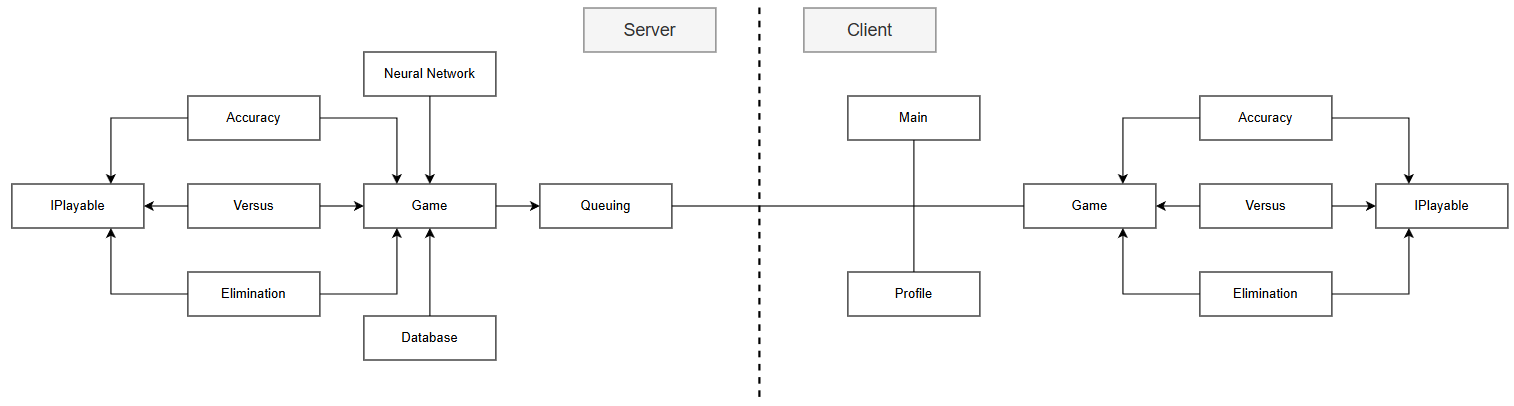
\includegraphics[width=1\linewidth]{resx/overview.png}
    \caption{High-level overview of components}
\end{figure}

The client communicates to the server through the \textbf{Connection} class which forwards requests related to a game to the \textbf{Queueing} class. This class contains a list of the current games, which it uses to relay the user's requests through to the appropriate game. The abstract game class can directly access the database and neural network, which it uses to evaluate a user's submission and save these results in a table. \\

The client has a designated class for each menu the application contains, which include the `Home' page, the `Profile' page, and when the user is playing a game.

\subsection{Choice of Language and Libraries} % // this is not good, maybe just rewrite

Since object-oriented programming is a necessary paradigm to use, C\# will be the most suitable language for this project. This also allows for the use of Windows Forms to create the UI for the client, and SignalR to provide a client-server connection. I have significant experience in both of these softwares, hence why they are suitable for the technical solution. \\

As discussed, the most suitable option for networking is the SignalR library from ASP.NET, as it allows for easy configuration and simple invokation of methods. I also require the System.Cryptography library in order to store passwords securely in the SQL database. I intend to use SHA512 encryption to hash the passwords, such that the plaintext passwords are not stored anywhere. \\

Since the solution requires a neural network, a method of multiplying matrices is necessary. As described in Objective 1.4.2, it is better to use the MathNet.Numerics library in order to perform the forward pass of the network. \\

As part of the UI design, I have chosen to use the Guna.UI2.WinForms package as it offers a wider variety of controls than the base Windows Forms.

\newpage
\hiddensection{Server Design}
\noindent\rule{\textwidth}{0.2pt}

\subsection{Neural Network}

The neural network consists of four classes, each of which perform a core function of the network. The \textbf{Network} class performs the forward pass, which is used to evaluate a user's submission. The \textbf{Backpropagation} class is used to train the network, and therefore will contain instances of the \textbf{Network} class. Both of these classes frequently use the static \textbf{Data} class, which contains methods for saving and loading the network parameters. It also contains any mathematical functions, such as sigmoid. The \textbf{Training} class oversees the training process, and is responsible for feeding images and labels into the \textbf{Backpropagation} class.

\subsubsection{Forward Propagation}

Forward propagation in the neural network is managed by the \textbf{Network} class. This class contains two constructors, depending on whether a new set of weights and biases should be used. The \textbf{Data} class includes static attributes which store the network parameters as arrays of arrays. When this class is first accessed, the weights and biases are loaded from their respective files and stored in these attributes. The static `BuildMatrices()' method of the class is then called which creates the Matrix and Vector objects for each layer of parameters in the network, which are stored in static arrays. \\

If the constructor arguments include a new set of network parameters, then the `BuildMatrices()' method of the \textbf{Data} class is called with the parameters passed as arguments. This updates the Matrix and Vector objects to represent the new set of weights and biases. This constructor is always used when the network is being trained using the \textbf{Backpropagation} class, since the parameters are update after each iteration. \\

Both constructors then call the `EvaluateNetwork()' subroutine, which performs the forward pass. The program iterates through each layer excluding the input layer and creates a Vector object from the 1D array of the activated values for the previous layer. The equation outlined in 1.7.4.1 is then applied to these objects, where \(z\), \(w\), and \(b\) represent the neuron values, weights, and biases respectively. The Matrix and Vector objects which represent the network parameters are stored as static attributes in the \textbf{Data} class.

\begin{equation*}
    z^L=z^{L-1}\cdot w^L+b^L
\end{equation*}

The activated values for the current layer are then calculated using the neuron values. If the current layer is a hidden layer, then the sigmoid function is used to normalise the values. The sigmoid function is part of the \textbf{Data} class, which is accessed by static reference and returns the activated value for a neuron. Each neuron in the current layer is passed through this subroutine, and the resulting activated values are stored in a 1D array. The `AsArray()' method is used to directly extract the underlying array of the Vector class, instead of creating a new array.

\begin{figure}[H]
    \centering
    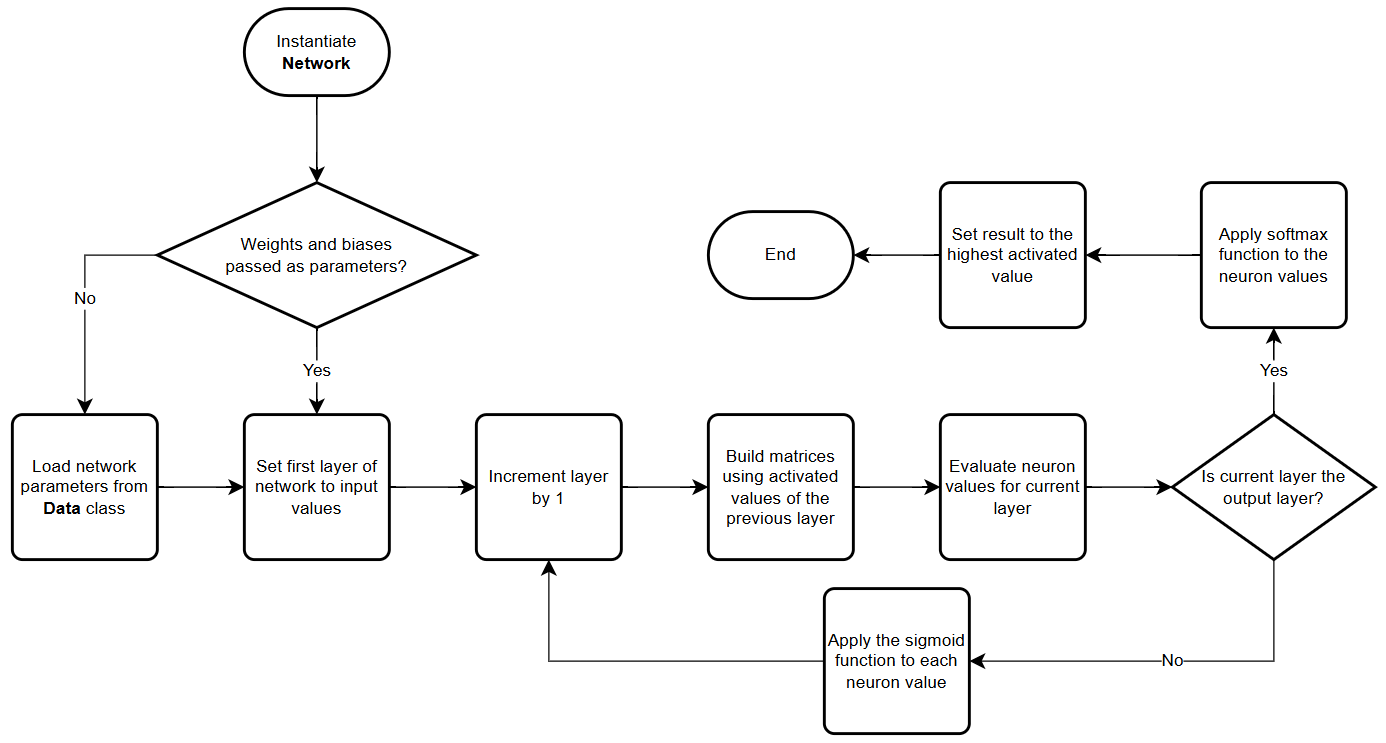
\includegraphics[width=1\linewidth]{resx/forward_pass.png}
    \caption{Flowchart detailing the forward pass of the neural network}
\end{figure}

The use of static Maxtrix and Vector objects in the \textbf{Data} class was not something incorporated in the prototype, which instead created the objects required for the current layer on each pass. This process was inefficient for the memory usage of the server---the new approach uses around 30 megabytes less memory during runtime.

\begin{center}
\rule{0.5\linewidth}{0.4pt}
\end{center}

\noindent The pseudocode below outlines the forward pass of the network:

\begin{minted}{csharp}
    func EvaluateNetwork() {
        foreach (layer in network_layers) {
            neuronsMatrix = BuildMatrix(activatedValues[layer---1])
            neuronValues[layer] = (neuronsMatrix * weightsMatrix + biasesMatrix)

            if (layer is output_layer) {
                activatedValues[layer] = Softmax(neuronValues[layer])
            }
            else {
                foreach (neuron in layer) {
                    activatedValues[layer][neuron] = Sigmoid(neuronValues[layer][neuron])
                }
            }
        }

        maxValue, maxIndex = -1, -1
        foreach (neuron in output_layer) {
            if (activatedValues[output_layer][neuron] > maxValue) {
                maxValue, maxIndex = activatedValues[output_layer][neuron], neuron
            }
        }
        result = maxIndex
    }
\end{minted}

\subsubsection{Backpropagation}

Backpropagation is the process by which the parameters for the network are optimised to accurately evaluate a user's submission. The \textbf{Backpropagation} class is constructed with a batch of training data, where the size of the batch is assigned to a variable. The weights and biases for the network are then loaded using the methods in the \textbf{Data} class. The flowchart below outlines the general process for performing the backpropagation algorithm. \\

% // i don't even know how i messed this one up
\begin{figure}[H]
    \centering
    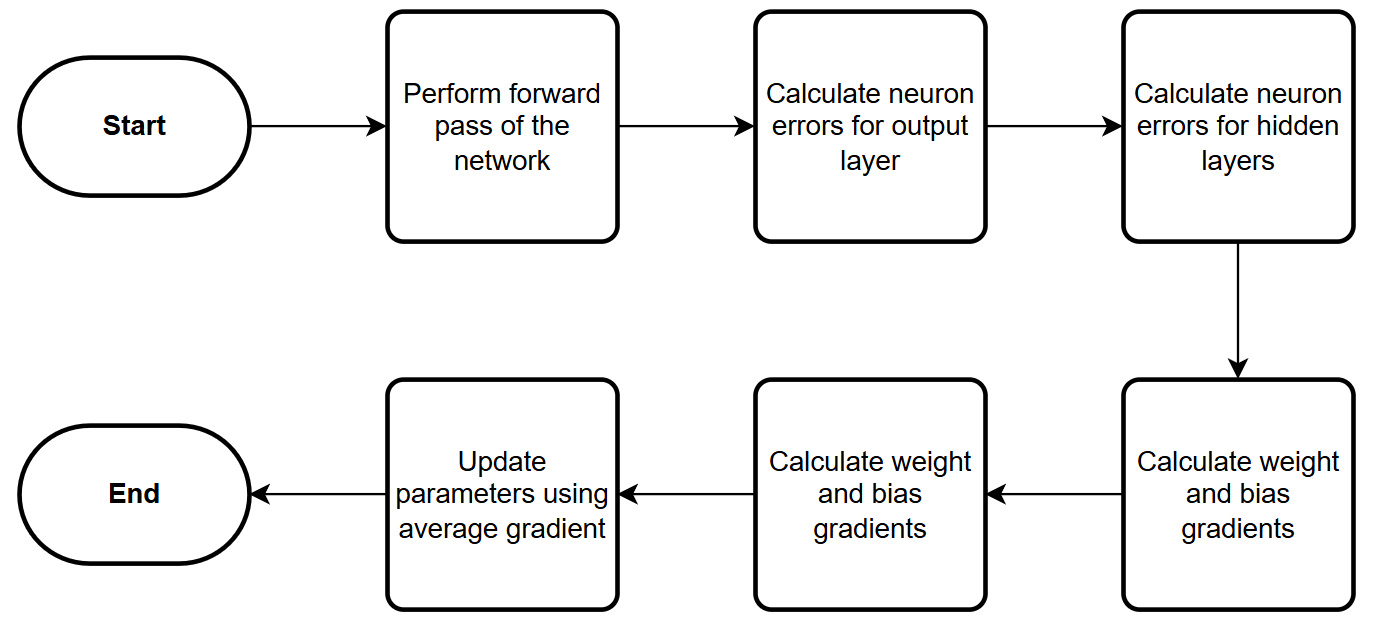
\includegraphics[width=0.75\linewidth]{resx/flow_backprop.png}
    \caption{Flowchart detailing the implementation of the backpropagation algorithm}
\end{figure}

The program then iterates through each set of images and labels, and applies the backpropagation algorithm to these sets. A new instance of the \textbf{Network} class is instantiated, passing in the input values and network parameters. If the result of the network correctly matches the label of the image then a counter is incremented. A second counter is incremented regardless of this condition, in order to produce an accuracy percentage. \\

The neuron errors for the output layer are then calculated using the expected result of the network. The softmax error function is applied to each neuron in the layer, which is equal to the derivative of the mean-squared loss function. The loss is also calculated and returned, as an indication of the rate at which the network is learning.

\begin{equation*}
    \delta^L_i=2(a^L_i-y)
\end{equation*}

The neuron errors for the hidden layers are then calculated using the errors from the previous layer. The program iterates through each reminaing layer, excluding the input layer and applies the sigmoid error function to each neuron. Each neuron error in the next layer is multiplied by the weight connecting it to the current neuron in the current layer. These values are summed for each neuron in the next layer which the current neuron connects to. This sum is then multiplied by the result of applying the derivative of the sigmoid function to the neuron value. \\

\begin{figure}[H]
    \centering
    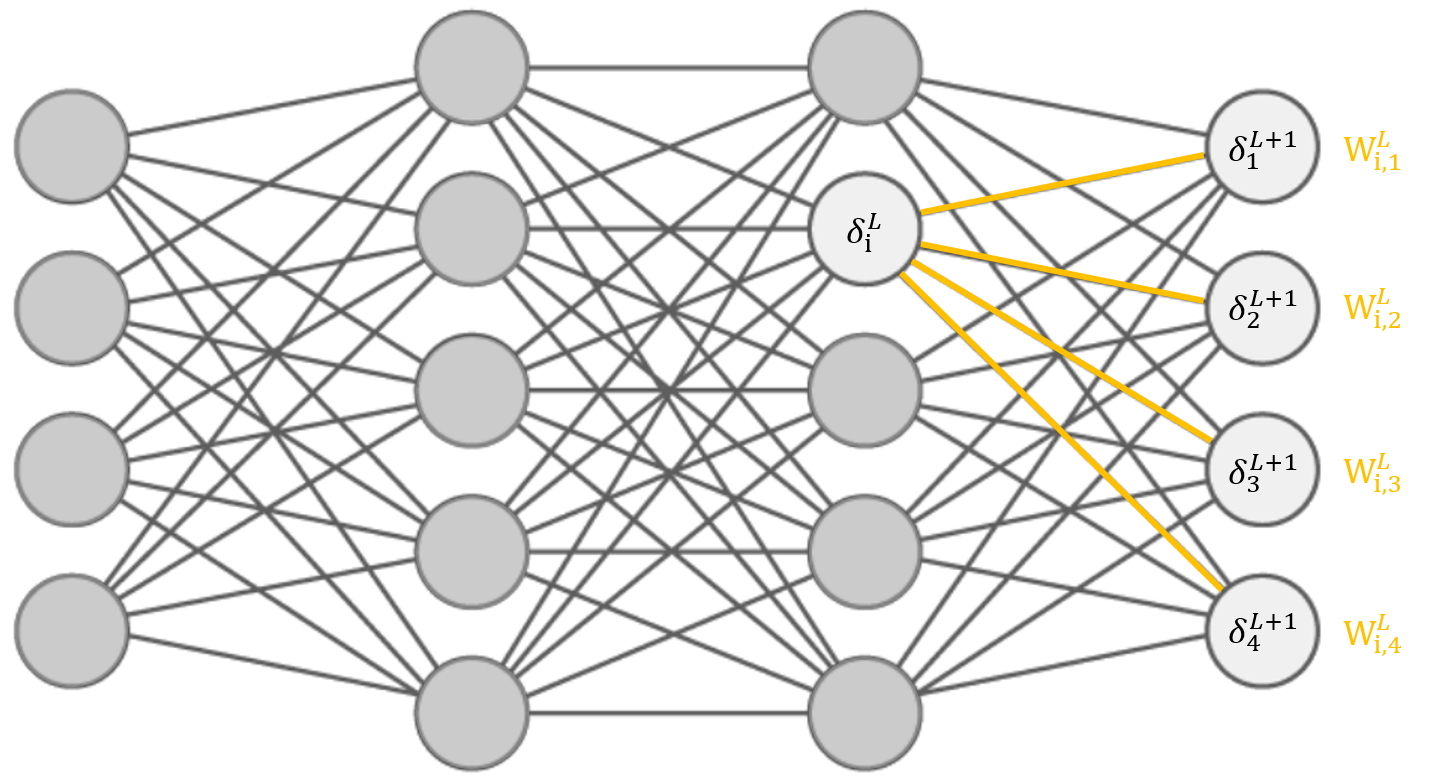
\includegraphics[width=0.75\linewidth]{resx/backpropagation_pptx.png}
    \caption{The product of the weights and neuron errors are summed across all connected neurons}
\end{figure}

Once all the neuron errors have been calculated, the gradients for the network parameters can be calculated. These represent the multi-dimensional `direction' which minimises the cost function the quickest. The bias gradients are equal to the neuron errors, so no further calculations have to be made. For the weight gradients, the program iterates through each weight in the network. The gradient for a specific weight is the product of the activated value passed through it and the neuron error of the neuron it connects to. These gradients are then returned and appended to a list of the adjustments to the network parameters for each image in the current batch.

\begin{equation*}
    \frac{\partial C}{\partial W_{i, j}^L} = \delta^{L+1}_j\cdot a^L_i 
\end{equation*}

After the backpropagation algorithm has been applied to all of the images in the current batch, the average gradient for each network parameter is calculated from the lists of adjustments, \(W\) and \(B\). This is done by iterating through each of the weights and biases, and summing all of the adjustments to the current parameter.

\begin{equation*}
    w'^L_{i,j}=w^L_{i,j}-\frac{\text{learning rate}}{\text{batch count}}\cdot\sum W^L_{i,j}
\end{equation*}
\begin{equation*}
    b'^L_i=b^L_i-\frac{\text{learning rate}}{\text{batch count}}\cdot\sum B^L_i
\end{equation*}

\vspace{1em}

These averages are then multiplied by the learning rate, and each resulting gradient is subtracted from the current value of the parameter. The updated network parameters are then saved to the respective files using methods from the \textbf{Data} class. The average accuracy and loss for the current batch are also logged to the console.

\begin{center}
\rule{0.5\linewidth}{0.4pt}
\end{center}

\noindent The pseudocode below outlines the general process behind the backpropagation algorithm
\begin{minted}{csharp}
    func Backpropagation(inputImages, expectedValues) {
        batchCount = inputImages.Count

        foreach (image in inputImages) {
            weightGradients, biasGradients, loss = Backpropagate(image, expected, weights, biases)

            weightAdjustments.Add(weightGradients)
            biasAdjustments.Add(biasGradients)
            losses.Add(loss)
        }

        upatedWeights = UpdateWeights(weights, weightAdjustments)
        updatedBiases = UpdateBiases(biases, biasAdjustments)

        SaveWeights(updatedWeights)
        SaveBiases(updatedBiases)
    }

    func Backpropagate(input, expected, weights, biases) {
        network = new Network(input, weights, biases)

        loss = CalculateOutputErrors(network, expected)
        CalculateHiddenErrors(network, weights)

        foreach (layer in network) {
            foreach (weight in layer) {
                weightGradients[layer][weight] = neuronErrors[layer + 1][weight] *
                                                 activatedValues[layer][weight]
            }
        }
        
        return (weightGradients, neuronErrors, loss)
    }
\end{minted}

    % func UpdateWeights(weights, weightAdjustments) {
    %     foreach (layer in network) {
    %         foreach (weight in layer) {
    %             weightSum = 0
    %             foreach (adjustment in weightAdjustments) {
    %                 weightSum += adjustment[layer][weight]
    %             }
    %             weights[layer][weight] -= (learningRate / batchCount) * weightSum
    %         }
    %     }
    %     return weights
    % }

    % func UpdateBiases(biases, biasAdjustments) {
    %     foreach (layer in network) {
    %         foreach (bias in layer) {
    %             biasSum = 0
    %             foreach (adjustment in biasAdjustments) {
    %                 biasSum += adjustment[layer][bias]
    %             }
    %             biases[layer][bias] -= (learningRate / batchCount) * biasSum
    %         }
    %     }
    %     return biases;
    % }

\noindent The pseudocode below details how calculating the neuron errors can be implemented. These functions are implementations of their equivalent functions in the previous pseudocode block. The implementations of `UpdateWeights()' and `UpdateBiases()' have not been included as pseudocode, since the processes are simply computing a mean average.
\begin{minted}{csharp}
    func CalculateOutputErrors(network, expected) {
        foreach (neuron in output_layer) {
            y = 1 if expected == neuron else 0
            loss += (activatedValues[neuron]---y)^2
            neuronErrors[output_layer][neuron] = 2 * (activatedValues[neuron]---y)
        }
        return loss
    }

    func CalculateHiddenErrors(network, weights) {
        foreach (layer in hidden_layer) {
            foreach (neuron in layer) {
                sum = 0
                foreach (error in neuronErrors[layer + 1]) {
                    sum += weights[layer][neuron] * error
                }
                neuronErrors[layer][neuron] = sum * dx_Sigmoid(neuronValues[layer][neuron])
            }
        }
    }
\end{minted}

\subsubsection{Image Preprocessing}

The image submitted by a user may not conform to the standards of the training data. When a submission is received, it is preprocessed by the `PreprocessImage()' method of the \textbf{Data} class. This performs three steps on the submitted image: cropping to the Region of Interest (ROI), extending the image dimensions, and adding padding around the ROI.\@ The resulting \(28\times 28\) image is then converted to an array of real numbers between 0 and 1 depending on the brightness of each pixel. \\

The ROI is determined by pixels which are not white. A pointer is created for each axis-aligned direction which points at the furthest non-white pixel in the given direction. These are found by iterating through each pixel and updating these pointers if their position exceeds the current value of the pointer. A failsafe also exists for an empty image which returns the original image, since the initial value of the pointers are not valid for an image. Otherwise, a new Bitmap is created with the dimensions cropped to the ROI and the same pixel format. \\

The dimensions of the cropped image are then adjusted such that the resulting image is a square. If the image is already a square, it is scaled down to \(24\times 24\) pixels and returned. Otherwise, the largest of the two dimensions is obtained using the `Math.Max()' function, and the image offset is set to the mean of the two dimensions. The direction which the image offset is to be applied is then set to the shorter of the two dimensions. A new bitmap is then created with both dimensions equal to the largest dimension of the cropped image, and its pixels are set to white. The method then iterates through each pixel in the new image and checks the pixel is not out of bounds of the cropped image. The pixel is then new image is then set to the pixel of the cropped image with the offset applied in the correct direction. The final image is then scaled to \(24\times 24\) pixels and returned as a new Bitmap.

\begin{minted}{csharp}
    if (i < image.Width && j < image.Height) {
        if (extendDirection == `w') {
            square.SetPixel(i + offset, j, image.GetPixel(i, j));
        }
        if (extendDirection == `h') {
            square.SetPixel(i, j + offset, image.GetPixel(i, j));
        }
    }
\end{minted}

The padding is then added to the \(24\times 24\) image as 2 white pixels on all sides. This is done by creating a new Bitmap with dimesions \(28\times 28\), which is filled with white pixels. The \(24\times 24\) image is then added to this image offset by (2, 2) which places it in the centre.

\subsubsection{Training}

Training a neural network involves feeding it through thousands of existing data, consisting of the image and its associated label. These are stored in GZip files, which can be read using the \textbf{GZipStream} class. When a new \textbf{Training} class is instantiated, it first loads the images and labels from their files. The training data contains 731,668 images and labels, so I opted to use the first 500,000 which although includes lowercase letters, these are discarded when the data is filtered.

\paragraph{File Loading\\}

First, a new `FileStream' object is created which points to the required GZip file. A new `GZipStream' can then be created using this object and setting the compression mode to decompress. The file contains metadata of length 16 bytes, so these bytes are discarded by the reader. The program then repeatedly reads exactly 784 bytes from the stream and creates a new 1D array to store these values. The values range from 0 to 255 which represents the brightness of a given pixel. These are normalised to values between 0 and 1 by dividing by 255 and assigning to a new array. The created image is then added to a list of images and the current progress of loading the images is logged to the console. \\

The labels are read in a similar way but have differences in the number of bytes to be read. The metadata for the labels is only 8 bytes long, so the reader discards 8 bytes instead of 16. The labels are only a byte long, so the program iterates through each label and appends each label to a byte array. These numbers range from 0 to 61, since the dataset includes digits, uppercase letters, and lowercase letters.

\paragraph{Filtering\\}

Once the images and labels have been loaded, the digits and lowercase letters need to be filtered out of the set, to leave only the uppercase letters. The `FilterImages()' method creates new lists for the filtered images and labels and iterates through each image-label pair in the full set of data. The uppercase letters have labels between 10 and 35, so if this condition is met, the current images and labels are appended to the filtered lists. The value of the label is adjusted so that they range from 1 to 26 instead of 10 to 35.

\paragraph{Sampling\\}

The program then iterates over the following sequence a set number of times, which represents the number of training iterations that will be performed. I have set this to the number of images divided by the size of a batch. \\

First a random integer is chosen between 0 and 50 less than the number of images. A range of 50 images and labels is then extracted from the filtered dataset, starting at the index chosen by the random integer. This set of 50 images and labels is then fed into the constructor of the \textbf{Backpropagation} class, which trains the network.

\subsubsection{Data Structures}

Since a neural network consists of complete bipartite graphs, a set of adjacency matrices can be used to represent the network. The weights can be stored in an array of 2D arrays where \(\text{weight}[L][i,\ j]\) references the weight between the \(i^{\text{th}}\) neuron in layer \(L\) and the \(j^{\text{th}}\) in layer \(L+1\). Similarly the biases can be stored in an array of 1D arrays where \(\text{bias}[L][i]\) references the bias of the \(i^{\text{th}}\) neuron in layer \(L\). This allows libraries to easily convert the parameters into a matrix and vector, which improves the speed of a forward pass. The neuron values, neuron errors, and activated values can be stored in the same way as the biases.

\subsubsection{File Organisation}

In order to save and load the network parameters, I opted to store the values as plaintext. I formatted the values as separated by commas and linebreaks, where each layer has its own file. For the weights, each line represents a single neuron where each comma separated value is an arc to a neuron in the next layer. The biases are stored in a single line, with commas separating the value for each neuron.
\subsubsection{UML Diagrams}

\begin{figure}[H] % // parameter arrays are private now
    \centering
    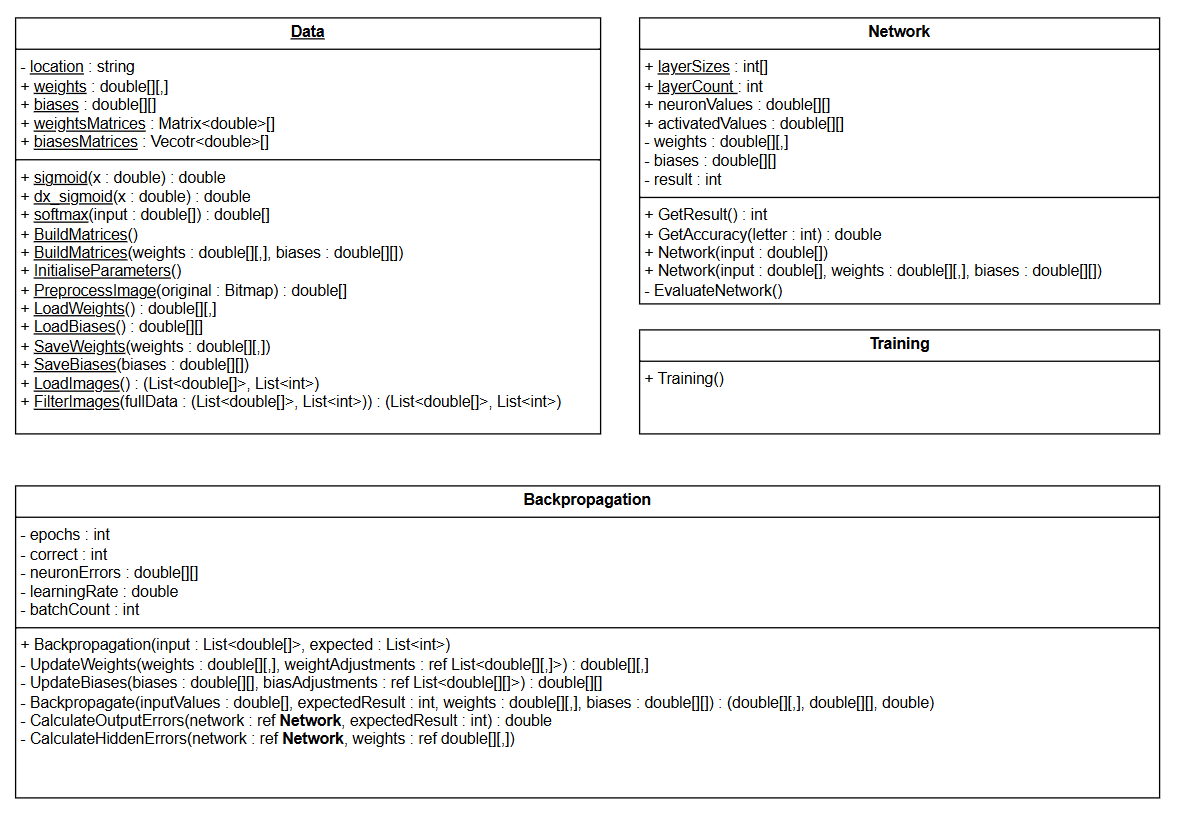
\includegraphics[width=1\linewidth]{resx/network_class.png}
    \caption{Class diagram for the neural network classes}   
\end{figure}

\subsection{Games}

There are three different game types I will implement in the technical solution. Each of these will inherit a base class for an abstracted game type, and an interface identified by IPlayable. The base class will include modules which are common across all game types, and also ones which can be overriden in order to extend their functionality. \\

The IPlayable interface consists of subroutines which make up the core functionality of a game. This is to allow different `phases' of a game to be called from outside the class, such as when a client submission is received. It also provides methods for retrieving information about the game, such as its type or the number of players currently queued into it.

\begin{minted}{csharp}
    interface IPlayable
    {
        bool QueueUser(string userID);
        bool DequeueUser(string userID);
        Task UpdateUsers();
        Task StartGame();
        Task SubmissionPhase();
        void LoadResponse(string userID, byte[] input);
        void EvaluationPhase(char letter);
        Task ContinueRequest(string userID);
        void EndGame();
        Games GetGameType();
        string GetGameID();
        bool HasStarted();
        int GetPlayerCount();
        int GetMaxPlayers();
    }
\end{minted}

An enumerable type with the identifier `Games' is used to differentiate between game types, where the abstract game class will include a protected attribute of this enumerable. This is used when queueing users into the requested game type. It should be noted that the name of each game has changed since the Modelling section of Analysis was conducted.

\begin{minted}{csharp}
    enum Games
    {
        Accuracy,
        Versus,
        Elimination,
    }
\end{minted}

The currently active games are stored in a list of the IPlayable type in the \textbf{Queueing} class, which allows it access to the public `get' methods of a game. This allows the class to appropriately queue a user when a request is made.

\subsubsection{Queueing}

When a user queues a game, they provide the game type as an enumerable and their userID.\@ The \textbf{Connection} class forwards this request to the \textbf{Queueing} class and additionally provides the IHubContext of the \textbf{Connection} class, which allows for communication with the client from within the game class. By iterating through each game in the list of current games, a suitable game may be chosen if it meets the required criteria.

\begin{itemize}
    \item The type of the game must match the requested type by the client
    \item The number of players in the game must be less than its maximum capacity
    \item The game must have not started yet
\end{itemize}

If a suitable game is found, the user is queued into the game using the methods available through the interface. This method returns the gameID as a string, which is used to uniquely identify the game when the user leaves the game, since the users in a game is not a public attribute nor available through the interface. \\

If no suitable game can be found, a new game of the requested type is instantiated. This is implemented by creating a new `IPlayable' object, which is assigned the instance of the requested game class using a switch statement on the enumerable `Games'. In the unlikely event that the value of the enumerable passed by the client does not match a valid game, an exception is immediately thrown. This can only occur if the possible game types registered differs between the server and the client. \\

The userID and IHubContext are passed as constructor arguments, where the userID is used along with the current time to create the gameID.\@ The new game is added to the list of active games, and the user is queued into the game using the interface method. \\

After a user has been successfully queued into a game, the gameID is returned to the client which then sends a confirmation to the server. When a user joins a game, the list of users for every user in the game needs to be updated. However if this method is called when a user queues, it causes the client to try and render the list of users before it has loaded the game. The confirmation alleviates this issue by only calling `UpdateUsers()' once the confirmation has been received. \\

A user can dequeue from a game either by closing the application or clicking the `Home' button. Regardless, a request is made to the server to dequeue the user from the current game, which is provided by passing the gameID as a parameter. Once the user has been dequeued, the `UpdateUsers()' method is called. If the user leaving the game results in the game having zero users in it, then it is disposed and removed from the list of current games. The `Elimination' game type overrides the method to dequeue a user and additionally removed the userID from the list of alive users.

\begin{figure}[H]
    \centering
    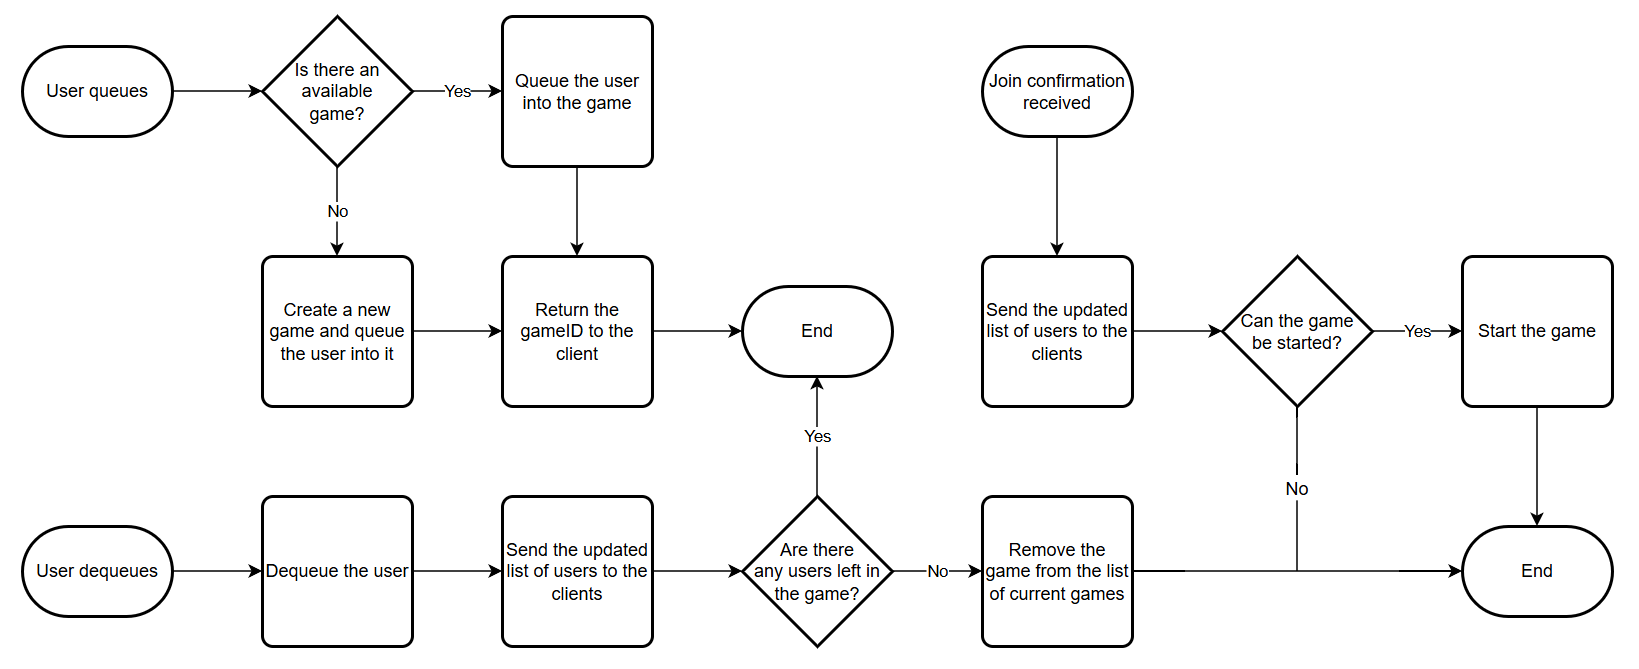
\includegraphics[width=1\linewidth]{resx/queue_flow.png}
    \caption{Logic of queueing, dequeueing, and join confirmations}   
\end{figure}

\subsubsection{Game Logic}

The constructor for each game type has no body, and only calls the base class constructor with additional paramaters to the userID and IHubContext. The game type as an enumerable is passed, along with the maximum number of players for the specific game type. \\

The base class then creates the gameID, and sets the appropriate protected attributes of the class to the constructor parameters. The protected instantiated attributes also have a value assigned to their allocated memory, such as the list of users and their userData, and the responses and continue requests for a round. The userDatas in a game are stored as a list of `friendData' structures, since the game only requires the rank of a user. A boolean value is set to false which indicates if the game has started, and the number of rounds that have occured is set to zero. \\

Each game contains a dictionary of a structure which stores the statistics for a single user. Each userID is mapped to their statistics for the current game, which are stored as lists of accuracies and elapsed times. The structure contains a method which updates these statistics by passing in the results for a given round.

\paragraph{Queueing\\}

When a user is queued into a game from the \textbf{Queueing} class, the user's rank is loaded from the database using the friendData structure and added to the list of userDatas, as well as the list of users. If the database fails to retrieve the relevant information, then the method returns false. This is propogated back through the call stack, eventually sending an error message to the client. \\

To dequeue a user, their userData and userID are removed from the relevant lists. This method also returns false if the userData of the user cannot be found in the list, however the calling method does not handle this exception. \\

When the \textbf{Queueing} class queues or dequeues a user, it also accesses a method to update the users through the interface. This sends an updated list to the users already in the game which causes them to refresh the list of users on the client application.

\paragraph{Game Start\\}

The method used to start a game is called from the \textbf{Queueing} class when a user join acknowledgement is received. Each game type has a unique implementation of this method, where calling the base method followed by calling the submission phase is common across all game types. \\

The base method sets the boolean value to represent if the game has started to true, and creates a new `gameStats' object for each user to store the results for the current game. A message is then sent to the clients to set up the application for the first round. After five seconds, a second messages is broadcasted which signals that the game is now starting. \\

The `Accuracy' game type uses the `GenerateLetters()' method in the abstract class to randomly generate 10 letters for the game. The `Versus' game type additionally sets the score of each user to zero, and caches the userData for both users so the Elo rating of each is updated even if they dequeue. The `Elimination' game type does not generate any letters and instead copies the list of users into a new list which contains the alive users.

\paragraph{Submission Phase\\}

Each game type has a unique implementation for the submission phase of the game, and there is no base method to override. The submission phase is where a letter is sent to the clients, and their responses are recorded. \\

For the `Accuracy' and `Versus' game types, the game is ended if the number of rounds played is equal to the set number of rounds for that game. Otherwise, the list containing the requests to continue to the next round is cleared, and the `AwaitRound()' method is called which sends a message to the clients for a countdown to be started for the next round. After three seconds, the current time is recorded, and the list of user submissions is cleared. The `SendLetter()' method from the base class is then called, with the users and current letter passed in. \\

The `Elimination' game type additionally overrides the `AwaitRound()' method, since only the alive users should be able to play in the current round. For its implementation of the submission phase, the condition to end the game is if the number of alive users is equal to one. The letter for the current round is also generated, and broadcasted to the clients. \\

When a user submission is received by the \textbf{Connection} class as a byte array, it is forwarded to the \textbf{Queueing} class to allocate it to the associate game class. The base method for `LoadResponse()' converts the byte array to a Bitmap and preprocesses the image using the static method from the \textbf{Data} class. This returns an array which it adds to the dictionary of reponses for the current round, with the userID as the key, and a tuple of the array and the current time as the value. This allows the elapsed time the user spent on their submission to be calculated. \\

Each game type extends the functionality of the `LoadResponse()' method, and checks if all the expected responses have been received. This differs in the `Elimination' game type, hence why each has their own implementation. If all the user submissions have been received, then the evaluation phase is called.

\paragraph{Evaluation Phase\\}

Each game type has their own implementation of the `EvaluationPhase()' method, with no base method to override. All of the game types use the `EvaluateSubmission()' method in the base class, which creates a new \textbf{Network} class to evaluate the user's submission. The result of the network is compared to the current letter to determine if the user was correct, which is returned as a boolean value. The elapsed time is calculated as the difference between the time the submission was recieved and the start time of the current round. The accuracy is extracted from the neural network as the activated value of the appropriate neuron for the given letter. The statistics for the current round are then added to the statistics structure for the user. \\

The `Accuracy' game type first creates an array of the \textbf{Network} class with the size equal to the number of users in the game. It then iterates through each user and evaluates their submission using the base class method, before sending the results to the client with the `SendResult()' method. The number of rounds played is then incremented. \\

The `Versus' game type applies the same process as before for evaluating the users' submissions. However it also utilises the return value of the `EvaluateSubmission()' method, and adds these users to a list of correct users. If this list has zero users in it, then the round is a draw, and each user is given a score of 0.5. Otherwise, the user with the lowest time and who is also in the correct users list is given a score of 1, and the other user is given a score of zero. The number of rounds played is incremented and the specific results for the `Versus' game are also sent, which include the user who won the round. \\

The `Elimination' game type is similar, however creates a list of incorrect users instead. If this list is empty, then the user with the longest time is added to a local list of eliminated users and removed from the list of alive users. Otherwise, if the number of incorrect users is less than then number of alive users, then these users are eliminated from the game. The specific results for the `Elimination' game are then sent to the clients with a list of the alive users, which allows the client to refresh their list of users and determine if they were eliminated. This is only broadcasted to the alive users, and user who were eliminated in the current round, since users eliminated in a previous round should not receive these results. \\

When the client application loads the results for the current round, it loads a `Continue' button. If a user presses this button it is received by the \textbf{Connection} class and forwarded to the appropriate game through the \textbf{Queueing} class. The userID is added to a list of continue requests, after checking that the user has not already clicked the button in the current round. If the size of the continue requests list is then equal to the number of users in the game then a new submission phase is started which loads the next round of the game. The `Elimination' game type will check if its size is equal to the number of alive users, rather than the total number of users.

\paragraph{Game End\\}

The conditions to determine if a game should end are checked in the submission phase method, which calls the `EndGame()' method if the conditions are met. The `Versus' game type extends the functionality of this method, in order to recalculate the users' Elo ratings. \\

First, a message is sent to all the users that the game has ended, to allow the client application to load the `Game End' screen. The program then iterates through each user and iterates through each round that the user completed, since this varies in the `Elimination' game type. The user's userData is loaded from the database and the `UpdateStatistics()' method is called, passing in the userData, current letter and the current round index as parameters. This takes the loaded statistics from the database for the current letter, and updates them with the new results. These new values are then inserted into the database, and a message is sent to the current user containing a `statistics' structure of the current letter. \\

The `Versus' game type updates each user's Elo rating before calling the base method. The program iterates through each user and calculates their expected score, and thereby their updated rank using the appropriate K-factor. The current rating for the user is obtained from the cached userData from when the game was started. The database is then updated with this new rating, which is also sent to the user.

\subsubsection{Data structures} % //

Each game class instance contains a list of the users who are queued into the game, as well as an integer for the maximum number of users that can join the game. A game also contains a unique ID which allows user submissions to be sent to the correct class instance. \\

In each game there is a dictionary which stores the statistics for every user. The key is a string value representing the userID, and the value is a structure. This contains a set of values for each letter completed: whether the user was correct, their accuracy, and the time it took them. The structure also contains a subroutine to update these values during the evaluation phase.

\begin{minted}{csharp}
    public struct gameStats
    {
        public List<bool> correct;
        public List<double> accuracy;
        public List<TimeSpan> time;

        public void update(double accuracy, TimeSpan time, bool correct)
    }
\end{minted}

For every round, there exists a Dictionary `currentResponses' which stores the users' submissions during the submission phase. The key is set to the userID of the submission, and the value is a tuple containing both the time of submission and an array containing the image data.

\subsubsection{Object-Oriented Design} % // evalsub, buildmat

Each game type inherits methods and properties from the \textbf{Game} class, and implements the \textbf{IPlayable} interface. The \textbf{Game} class contains generic methods that each game utilises, and also implements some of the methods from the \textbf{IPlayable} interface. A number of its methods are virtual, which allows the specialised games to extend their base functionality. Each game contains a `gameStats' structure for each user, and the games are owned by the \textbf{Queueing} class. The associations between the classes has not be shown in the below figure, due to the complexity of the diagrams, and is instead shown in section 2.7.

\begin{figure}[H]
    \centering
    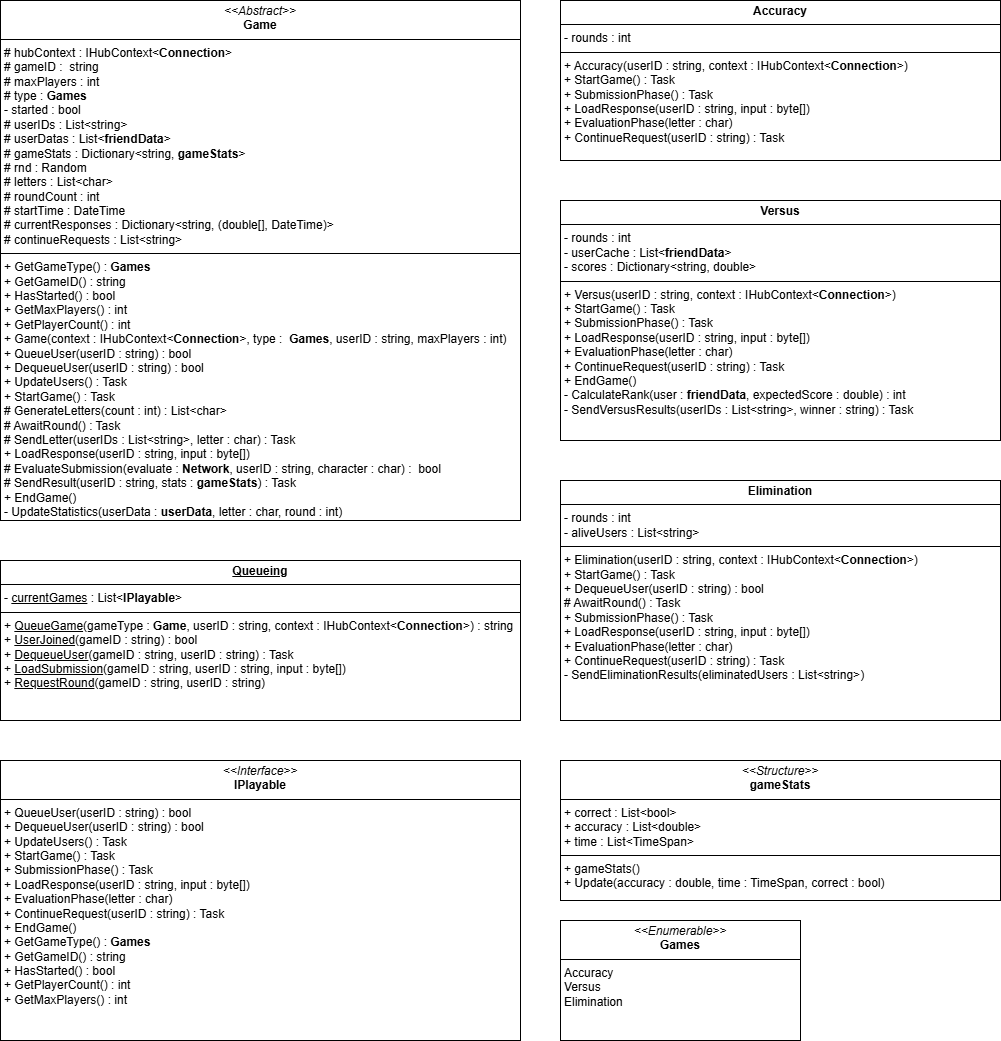
\includegraphics[width=1\linewidth]{resx/games_class.png}
    \caption{UML diagrams for the Game classes}
\end{figure}

\subsection{Database}

The SQL database is used to store user accounts, their details, and relationships with other accounts. There are four tables: `userData', `statistics', `friends', and `friend invites'. The `userData' table is used to store the account details of a user, which includes their login credentials, Elo rating, and localisation. Each user has 26 records detailing their statistics for each letter. As this is a one-to-many relationship, the `statistics' table stores these values, using the letter and userID as a primary key. The userID is also a foreign key, which links the statistics records to the account in the `userData' table. \\

The `friends' table creates a link between two userIDs, which represents that they have added each other as friends. Only one link exists per friendship which means extra logic is required to return the friends of a given user, since the user could be the first or the second user in the record. The `friend invites' table is used when a user sends a friend request but the receiving user is not online. The request is instead stored in this table, and sent to the receiving user when they next come online.

\subsubsection{Database Design}

Since each user has 26 statistics, the `userData' table exists in a one to many relationship with the `statistics' table. 

\begin{figure}[H]
    \centering
    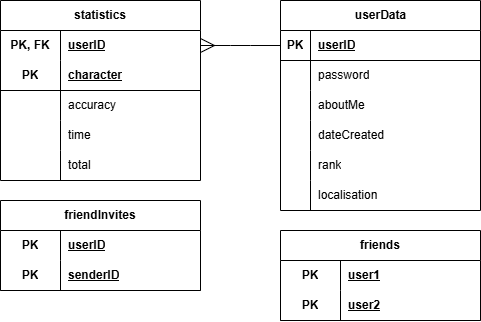
\includegraphics[width=0.5\linewidth]{resx/sql.png}
    \caption{ER diagram for the SQL database}
\end{figure}

\subsubsection{UML Diagram}

Access to the SQL database is controlled and managed by the static \textbf{Database} class, which contains the `SqliteConnection' object used to link the C\# class to the database file.

\begin{figure}[H]
    \centering
    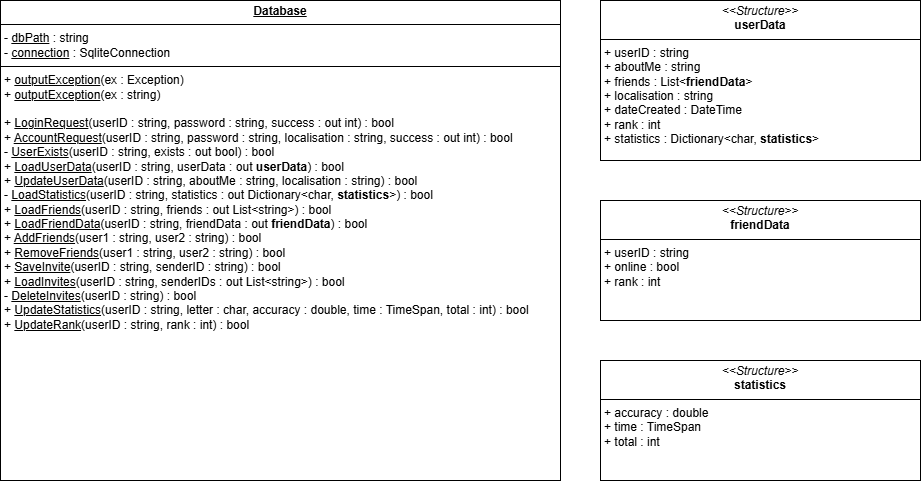
\includegraphics[width=1\linewidth]{resx/database_class.png}
    \caption{UML diagrams for the Database classes}
\end{figure}

\subsubsection{SQL Queries}

The \textbf{Database} class uses parameter queries to prevent SQL injections to the database. The parameters are recognised by the `@' symbol before the value, which are safely replaced by the requested data before each query is made. \\

Each method in the \textbf{Database} class returns a boolean value to represent if the query was successfully executed. If the method is requesting data from the database, then this is accessed by the calling method using the `out' keyword. When a method from the \textbf{Database} class is called, the SQL query for the method is allocated to a string value. The values which are to replaced by parameters passed in the method are prefixed with the `@'. The connection to the database is then opened and a new `SqliteCommand' object is instantiated with the query and `SqliteConnection' object as parameters. The arguements for the query are then injected into this object and the query is executed in the database. For an SQL command that writes to the database, the `ExecuteNonQuery()' method is used which does not return a value. For a command that reads from the database, the `ExecuteReader()' method is used which returns an `SqliteDataReader' object and is assigned to the `reader' variable.  If an expection occurs then the exception is logged to the console and the method returns false.

\begin{center}
\rule{0.5\linewidth}{0.4pt}
\end{center}

The `LoginRequest()' method gets the password for a user and compares it against the password passed as a parameter. The `success' of the login is initially set to 2 which represents a userID not existing in the database. The `reader' is then read in a while loop and will therefore not run if no rows are returned. If a row exists, the returned password stored in the database is compared to the one passed as a parameter and `success' is updated to 1 or 0 depending if the strings match. The password in the database is hashed, so the inputted password is hashed prior before it is passed into the `LoginRequest()' method. 
\begin{minted}{SQL}
    SELECT userData.password
    FROM userData
    WHERE userData.userID = @userID
\end{minted}
\begin{center}
\rule{0.5\linewidth}{0.4pt}
\end{center}

The `AccountRequest()' method attempts to create a new user account in the database along with empty statistics records for each letter. The method first employs the `UserExists()' subroutine to determine if the requested userID is already in use. The boolean representing this condition is an `out' parameter of the subroutine and is assigned to the `exists' variable. If the returned boolean of the subroutine is false, then an exception was thrown during the `UserExists()' method and this is propagated back by immediately setting `success' to -1 and returning false. Otherwise, the `exists' value is checked and `success' is set to 0 if the requested userID is present in the database, followed by returning true. \\

If the requested userID does not exist then a new account is created in the database with the values set to the passed parameters or their default values. The method then iterates from 0 through 25 in order to create new statistics records for the new user account. The letter stored in each record is given by adding 65 to the current iteration value and converting to a character type.
\begin{minted}{SQL}
    INSERT INTO userData
    VALUES (@userID, @password, @aboutMe, @dateCreated, @rank, @localisation)
\end{minted}
\begin{minted}[escapeinside=||]{SQL}
    INSERT INTO |statistics|
    VALUES(@userID, @letter, @accuracy, @|time|, @total)
\end{minted}
\begin{minted}{SQL}
    SELECT userID
    FROM userData
    WHERE userID = @userID
\end{minted}
\begin{center}
\rule{0.5\linewidth}{0.4pt}
\end{center}

The `LoadUserData()' method is used to load the account details of a user from the database and returns a `userData' structure. The `out' parameter storing the userData is instantiated and the `UserExists()' method is called. If an exception is thrown in this method then it will return false and this is propagated back by immediately returning false with the empty userData. If the user does not exist then an empty userData is still outputted but the method returns true. \\

Otherwise the account details are loaded from the `userData' table and allocated to the attributes in the `userData' structure. The `LoadStatistics()' and `LoadFriends()' methods are then called, which similarly propagate any thrown exceptions. A list of the `friendData' structure is then created, and the list of friendIDs is iterated through with the `LoadFriendData()' method called for each. This gets the Elo rating of the users, since their online status is determined otherwise.
\begin{minted}{SQL}
    SELECT aboutMe, dateCreated, rank, localisation
    FROM userData
    WHERE userData.userID = @userID
\end{minted}
\begin{minted}[escapeinside=||]{SQL}
    SELECT letter, accuracy, |time|, total
    FROM |statistics|
    WHERE userID = @userID
\end{minted}
\begin{minted}{SQL}
    SELECT user1, user2
    FROM friends
    WHERE user1 = @userID OR user2 = @userID
\end{minted}
\begin{minted}{SQL}
    SELECT rank
    FROM userData
    WHERE userID = @userID
\end{minted}
\begin{center}
\rule{0.5\linewidth}{0.4pt}
\end{center}

The `LoadInvites()' method is used to get all the friend invites for a user when they log into the application. A list is first created before the SQL query is executed. Each senderID in the returned rows is added to the list of invites. The invites are then deleted from the table since the user has now received them, using the `DeleteInvites()' method.
\begin{minted}{SQL}
    SELECT senderID
    FROM friendInvites
    WHERE userID = @userID
\end{minted}
\begin{minted}{SQL}
    DELETE FROM friendInvites
    WHERE userID = @userID
\end{minted}
% \begin{center}
% \rule{0.5\linewidth}{0.4pt}
% \end{center}

% \begin{minted}{SQL}
%     UPDATE userData
%     SET aboutMe = @aboutMe, localisation = @localisation
%     WHERE userID = @userID
% \end{minted}
% \begin{minted}{SQL}
%     INSERT INTO friends
%     VALUES (@user1, @user2)
% \end{minted}
% \begin{minted}{SQL}
%     DELETE FROM friends
%     WHERE (user1 = @user1 AND user2 = @user2) OR (user2 = @user1 AND user1 = @user2)
% \end{minted}
% \begin{minted}{SQL}
%     INSERT INTO friendInvites
%     VALUES (@userID, @senderID) 
% \end{minted}
% \begin{minted}[escapeinside=||]{SQL}
%     UPDATE |statistics|
%     SET accuracy = @accuracy, |time| = @|time|, total = @total
%     WHERE userID = @userID AND letter = @letter
% \end{minted}
% \begin{minted}{SQL}
%     UPDATE userData
%     SET rank = @rank
%     WHERE userID = @userID
% \end{minted}

\subsubsection{Security of Data}

In order to prevent database leaks exposing the passwords of users, a hashing algorithm is implemented. Instead of storing the password as plaintext, the hashed password is stored and this value is compared against when a user logs in. The hashing algorithm I chose to implement is SHA512 from the System.Cryptography library.

\subsection{Client-Server Connection}

For this project there are two classes which inherit the \textbf{Hub} class: \textbf{Accounts} and \textbf{Connection}. The \textbf{Accounts} class is only used to connect users in order to login or create an account. This seperates the functionality of a user who is logged in into a different class, enabling a Dictionary to be kept in the \textbf{Connection} class which maps a userID to their Context.ConnectionID.\@ The ConnectionIDs are used by SignalR to manage the address of each client and thereby communicate with them. \\

The \textbf{Games} class also requires communication with the clients but does not inherit the \textbf{Hub} class. Instead, dependency injection is used to provide the class with the IHubContext of the \textbf{Connection} class. This value is passed as a parameter into the constructor when a game is created.

\subsubsection{Server Configuration}

For the server to be able to communicate with a client, the server must have an open port where the `SignalR' package can listen to incoming requests. Due to previous experience with networking, the appropriate firewall controls already exist on the server machine for port 5252. NGINX is then used to examine the endpoint of the request and reassign its port number using reverse proxying. For this server application, I arbitrarily chose to use port 3900 as the port which `SignalR' listens to. The configuration of NGINX is shown below, which is adapted from the example given in the \href{https://nginx.org/en/docs/example.html}{documentation}.

\begin{minted}{nginx}
    listen 5252;
    
    location /cs-nea {
        proxy_pass http://localhost:3900;
    
        proxy_http_version 1.1;
        proxy_set_header Upgrade $http_upgrade;
        proxy_set_header Connection $connection_upgrade;
    
        proxy_set_header Host $host;
        proxy_set_header X-Real-IP $remote_addr;
        proxy_read_timeout 86400;
    }
\end{minted}

To configure the server, an `IHostBuilder' object is created using the `CreateDefaultBuilder()' method of the SignalR library and `SignalR' is added as a service to the host configuration. The configuration is set to use routing and the `IHubContext' of the \textbf{Connection} class is attributed to a public member in the class. This allows other classes to access the communciation methods which the SignalR library provides. The two endpoints are then mapped to their respective classes, such that any requests to the given endpoints will be received by the appropriate methods within that class.

CORS could also be set up to allow any origin to attempt a connection, which would allow devices outside of the server's LAN to communicate with the server. However this isn't very secure without proper implementation, and would need to be thouroughly researched. As a test, I did briefly start the server application with CORS enabled, however due to the setup of my home network this did not permit connections from outside the LAN.\@ This issue is further detailed in section 4.4.1, as I was not able to resolve it.

\begin{minted}{csharp}
    host-config {
        services {
            AddSignalR()
        }
        setup {
            UseRouting()
            hubContext = GetIHubContext<Connection>()
            endpoints {
                Connection => ("/cs-nea/connections")
                Accounts => ("/cs-nea/accounts")
            }
        }
        Logging = None
        UseUrls("http://localhost:3900")
    }
\end{minted}

The usage of NGINX allows the server application to bind to \textit{localhost} only. This is because the reverse proxying forwards any requests on port 5252 with the /cs-nea endpoint to the server, so it only needs to listen for the output of NGINX which is running on the same machine. This also means the server application is not directly exposed to the internet which improves security.

\subsubsection{UML Diagrams} % // HashPassword you melon like holy cases

For the `Accounts' and `Connection' classes, they contain methods which have zero references in the server application and are only invoked by the client. These have been shown by using camelCase rather than PascalCase as a naming convention.

\begin{figure}[H]
    \centering
    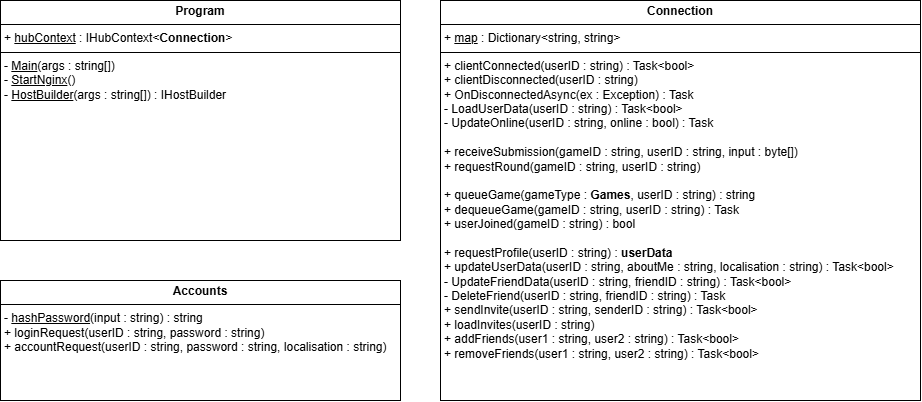
\includegraphics[width=1\linewidth]{resx/connection_class.png}
    \caption{UML diagrams for the Connection classes}
\end{figure}

\subsection{Object-Oriented Design}

The diagram below illustrates the relationships between all of the classes in the server application. 

\subsubsection{Class Diagram}

% evil and intimidating fully fledged class diagram with maximum aura
\begin{figure}[H]
    \centering
    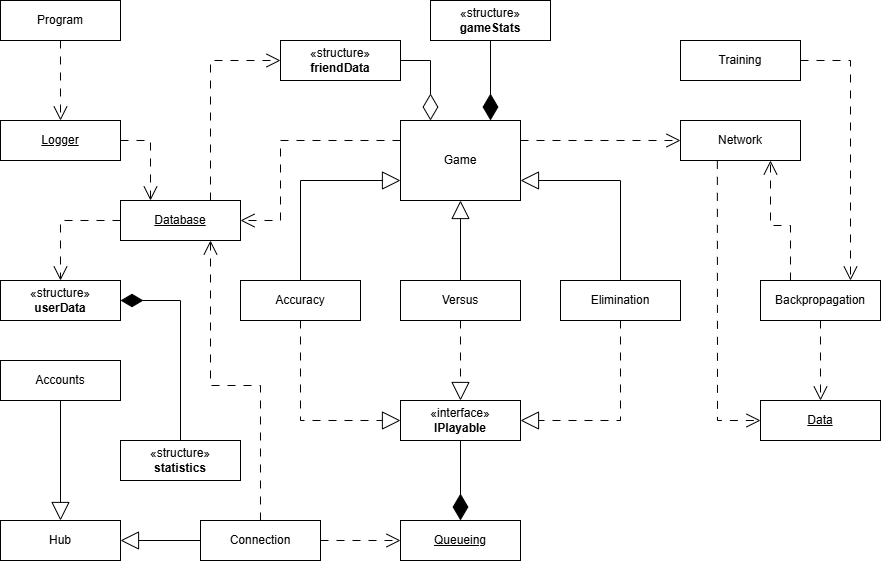
\includegraphics[width=1\linewidth]{resx/server-class-overview.png}
    \caption{Relationships between the server classes}
\end{figure}

\newpage
\hiddensection{Client Design}
\setcounter{subsection}{7}
\noindent\rule{\textwidth}{0.2pt}

\subsection{Client Menus}

The \textbf{Main} form class is instantiated by the \textbf{Login} form class when a successful login occurs. The constructor passes the userID of the account that has been logged into, and the language used by the \textbf{Login} form. The `localisation' field of the `userData' is then set to this language, since this field cannot be null while rendering the form. If the user's account language differs then the text is immediately updated once the userData has been loaded. The instance of the \textbf{Main} class is then injected into the \textbf{hub\_connection} class, which allows methods to be called from a server invokation. \\

The static `instantiateComponent()' method of the \textbf{UXelements} class is then called, which configures the basic layout of the form, which is consistent across all sub-menus. The `InitialiseConnection()' method is then called which creates a new `HubConnection' object, independent of the connection established by the \textbf{Login} class. The connection handles are then added to the object and the connection is started. The asynchronous `ConnectionClosed' method is attached to the event handler of the `HubConnection' object for the connection to the server being unexpectedly closed. The client then invokes the `clientConnected()' method on the server, passing the userID as a parameter.

\subsubsection{Accounts}

The client application creates a new \textbf{Login} form class on start, after loading the languages into a dictionary. The form is created and the elements are configured and displayed to the user. The input text boxes then have event handler assigned to them which resets the information label when their contents are edited. The text of the `language' button is then set to the current active language, using the supported languages list in the \textbf{Languages} class. \\

The instance of the \textbf{Login} form class is then injected into the static \textbf{hub\_connection} class, which it uses to call the appropriate subroutines of the class when a connection handler is invoked by the server. The `InitialiseConnection()' method is then called. \\

This subroutine configures a connection of the `HubConnection' type, then attaches the required handlers and attempts to start the connection---this process is detailed later in section 2.12. The asynchronous `ConnectionClosed' method is attached to the event handler of the `HubConnection' object for the connection to the server being unexpectedly closed. This start an attempt to reconnect, which updates the connection status label on the form to alert the user of the loss of connection. 

\paragraph{Login\\}

When the user clicks the `Login' button, the event handler for this button is called. This extracts the text stored in the username and password text boxes, and then resets the password text box. The credentials are then checked if they are empty or white space, terminating the subroutine if this is the case. Otherwise the `loginRequest()' method is invoked on the server to send the login request. \\

If the request is successfully handled, a response is received into the `loginSuccess' connection handler. A switch statement is then performed with the returned success code with the following possiblities:

\begin{itemize}
    \item VALID = 1
    \item INCORRECT\_PASSWORD = 0
    \item USER\_DOES\_NOT\_EXIST = 2
    \item USER\_LOGGED\_IN\_ON\_OTHER\_DEVICE = 3
    \item ERROR\_OCCURED = -1
\end{itemize}

If the returned success code is 1 indicating the login was successful, the main application is launched by initialising an instance of the \textbf{Main} class. The userID and language used in the login form is passed as a parameter, to allow the client to request the user's account data.

\paragraph{Account Creation\\}

If the user clicks the `Create Account' button, the `Login' button is moved down and the text is replaced with `Create Account'. A second password box is added which must have a matching password for the account to be successfully created. \\

When the user clicks the `Create Account' button, the event handler for this button is called. This extracts the text stored in the username and password text boxes, and then resets the password text boxes. If the passwords do not match, the user is informed of this through a message and the account request is not sent. Similar to the `Login' button, a check is performed to ensure the username or password boxes are not empty or white space. The client then invokes the `accountRequest()' method on the server, passing the username, password, and the current language. \\

If the request is successfully handled, a response is received into the `accountSuccess' connection handler. A switch statement is then performed with the returned success code with the following possiblities:

\begin{itemize}
    \item VALID = 1
    \item USERID\_TAKEN = 0
    \item ERROR\_OCCURED = -1
\end{itemize}

If the returned success code is 1 indicating the account creation was successful, the main application is launched by initialising an instance of the \textbf{Main} class. The userID and language used in the login form is passed as a parameter, to retain the language used by the \textbf{Login} form class in the main application.

\subsubsection{User Information}

When the client invokes the `clientConnected()' method on the server, the userData for the requested user is sent to the client which invokes the `ClientConnected()' method on the client. This passes the userData as a parameter, which is set to the static `userData' object in the \textbf{Main} class. The `InitialiseComponent()' method of the \textbf{Main} class is then called which loads the main menu onto the empty layout. \\

The userData for the current user can be updated, which is received by a connection handler and forwarded to the `UpdateUserData()' method. This passes the userID, about me, and localisation. If the userID matches the userID associate with the current client application, then the about me and localisation in the `userData' structure are updated. If the user is currently in-game then no changes are made, and if they are on the main menu a full refresh is performed by calling the click event handler for the `Home' button. If the `Profile' object in the `menus' structure is not null, then the refresh has to be performed manually. The page text is reset, which indicates which sub-menu the user is currently in. The `ConfigFriendsPanel()' and `ConfigUserDataPanel()' methods are then called to refresh the left and right panels with the new language. If the user is viewing their own profile, then the profile page is also refreshed.

\paragraph{Friends\\}

The `UpdateFriendData()' method is invoked by the server when a friend of the user updates their account data, or the user has added a friend. The method passes a `friendData' structure as a parameter, and iterates through each friend of the user. If one of these friends matches the userID in the passed friendData, then the current friend is updates with the new structure. Otherwise, the friend must be a new friend, so the structure is added to the list of friends. The friends panel is then refreshed if the user is not in-game. \\

If a friendship has been removed, the server invokes the `removeFriends' connection handler on the client application. This iterates through each friend of the user, and removes the appropriate friendData, breaking the loop after doing so. The friends panel is then refreshed if the user is not in-game. \\

When a user opens or closes the client application, as part of the `clientConnected()' method, the `UpdateOnline()' method is also called. This iterates through each friend of the user, and resends their friendData. The server invokes a connection handler, which forwards the request to the `UpdateOnline()' method in the client application. This method has a userID and a boolean value representing if the user is now online or not as parameters. The method iterates through each friendData and updates the `online' attribute of the appropriate friend. If the user is not currently in-game, the left panel is refreshed to display these changes.

\paragraph{Social\\}

A user can add and remove a friend through the `Profile' page of the user. When a user clicks the `Add Friend' button, the `sendInvite()' method is invoked on the server which passes the userID and the senderID.\@ The button is then disabled since a friend invite cannot be sent twice. If a user clicks the `Remove Friend' button, the button is disabled and the `removeFriends()' method is invoked on the server. \\

The invites for a user are forwarded when the user logs into their account. The server passes a list of userIDs by invoking the `receiveInvites' connection handler. The client creates a new \textbf{ConfirmForm} dialog box for each invite, and invokes the `addFriends()' method on the server if the user clicks `Accept'.

\subsubsection{Profiles}

The \textbf{Profile} form class manages the profile page and is constructed with the instance of the \textbf{Main} class and a `userData' structure. The `InitialiseComponent()' method is then called which configures the main panel to display the profile page. This includes the userID and an overview of their statistics. A panel is then configured which contains the user's average accuracy, time, and total for each letter.

\paragraph{Searching\\}

When the user clicks the `Search' button, the click event handler first extracts the text in the input text box. If the extracted string is not empty or whitespace, the textbox is reset and the `RequestProfile()' method is called. This method invokes the `requestProfile()' method on the server, which returns a `userData' structure. If the userID of this returned structure does not match the requested userID, then a message is shown to the user that the requested user does not exist. Otherwise, the page text is set to ``Profile'', and a new instance of the \textbf{Profile} class is created in the `menu' structure. The instance of the \textbf{Main} class is passed as a parameter, as well as the returned `userData' structure.

\paragraph{Algorithms\\}
Each user has an overview of their statistics which can be viewed both on the home page and in the profile page. This includes the total number of rounds they have played, their Elo rating, and their average overall accuracy. The Elo rating is obtained from the `userData' structure so no calculations are required. By iterating through each letter, the total rounds played can be summed. The average accuracy is calculated by summing the accuracies for each letter, and dividing by the number of letters. This is then multiplied by 100 to convert it to a percentage, and rounded to two decimal places.

\subsubsection{UML Diagrams}

The associations between the classes has not be shown in the figure below, due to the complexity of the diagrams, and is instead shown in section 2.11.

\begin{figure}[H]
    \centering
    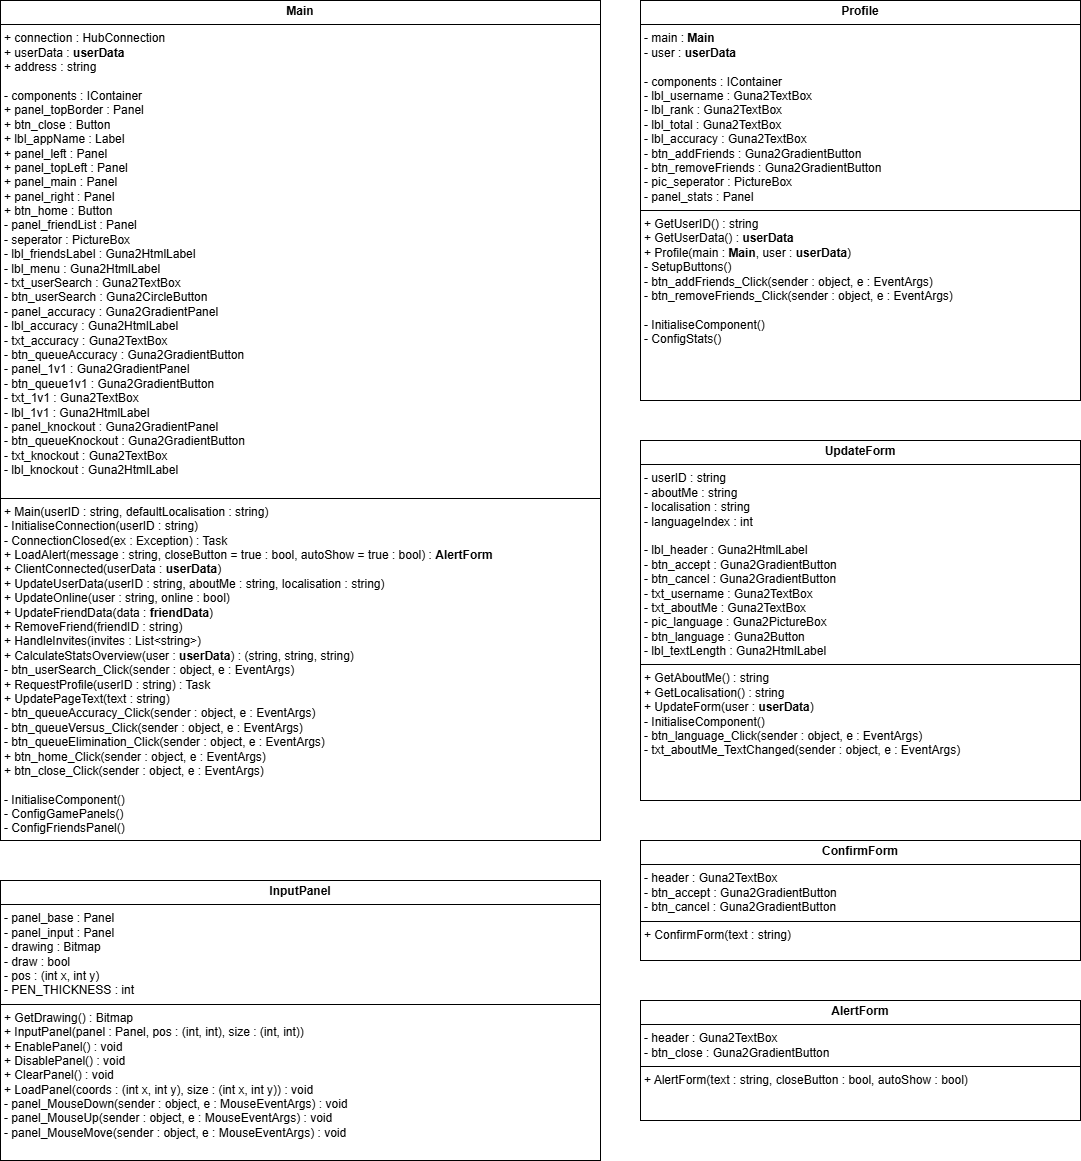
\includegraphics[width=1\linewidth]{resx/ui_class.png}
    \caption{UML diagrams for the Menu and Dialog classes}
\end{figure}

\subsection{Games}

As with the server application, the client application implements three different games types. These also inherit a base class for an abstracted game type, and an interface identified by IPlayable. The base class will include modules which are common across all game types, and also ones which can be overriden in order to extend their functionality. \\

The IPlayable interface consists of subroutines which make up the core functionality of a game. This is to allow different `phases' of a game to be called from outside the class, such as when a game to queue into is found. It also provides methods for retrieving information about the game, such as its type or the gameID.\@ \\

\begin{minted}{csharp}
    interface IPlayable
    {
        void QueueGame();
        Task JoinGameLobby();
        void AwaitStart();
        void StartGame();
        void AwaitRound();
        void SubmissionPhase(char letter);
        void EvaluationPhase(bool correct, double accuracy, TimeSpan time);
        void EndGame();
        void UpdateUsers(List<friendData> users);
        Games GetGameType();
        string GetGameID();
    }
\end{minted}

An enumerable type with the identifier `Games' is used to differentiate between game types, where the abstract game class will include a private attribute of this enumerable.

\begin{minted}{csharp}
    enum Games
    {
        Accuracy,
        Versus,
        Elimination,
    }
\end{minted}

The current game is stored in the `menu' structure, which contains the instances for the \textbf{Main} class, the \textbf{Profile} form, and the \textbf{IPlayable} interface.

\subsubsection{Queueing}

When a user clicks on the `Queue' button on the home screen, a new game for the specified type is instantiated. The constructor for the `Elimination' game type sets a boolean value to false representing if the user has been eliminated, and initialises the list of alive users. The remaining game types have empty bodies, and only call the base constructor. The instance of the \textbf{Main} form is passed as a parameter, to allow the game class to manipulate the Form controls. The base constructor is called with this instance, the game type as an enumerable, and the maximum number of players for the game type. \\

The `QueueGame()' method is then called, which first invokes the `queueGame()' method on the server and returns the gameID if the user was successfully queued. If the returned value is empty, then the user failed to be allocated to a game. Otherwise, the `JoinGameLobby()' method is called, which invokes the `userJoined()' method on the server, returning a boolean value representing if the user was successfully queued. \\

This also causes the server to invoke the `UpdateUsers()' method on the client, which updates the list of users. If the game has not started, then the lobby screen is configured and shown the user. Regardless of this, the left panel is updated with the new list of users. The `Elimination' game type overrides this method as it additionally seperates the users on whether they have been eliminated. Since this is only the case during the game, the `HasStarted()' method is used to determine if the game has started and will instead call the base method if it returns false. 

\subsubsection{Game Logic} % //
\paragraph{Game Start\\}

When the server invokes the `awaitStart' handler, the boolean value representing if the game has started is set to true. For the `Elimination' game type, each user is added to the list of alive users. A countdown is then configured to display to the user. Once the game has been started, the right panel is configured to display the round results. \\

When the server invokes the `awaitRound' handler, the main panel is configured and the drawing panel object is returned from the `ConfigGamePanel' method. The `clear' and `submit' buttons are then assigned click event handlers, and a second countdown is configured.

\paragraph{Submission Phase\\}

The submission phase is invoked after the client receives a letter. The number of rounds played is incremented, and the new letter is added to the list of letters. The drawing panel is then enabled using the `EnablePanel()' method, and the `submit' and `clear' buttons are enabled. \\

The `clear' button is allocated the `ClearPanel()' method of the drawing panel. The `submit' button disables itself and the `clear' button. It then calls the `DisablePanel' method of the drawing panel and gets the drawing from the panel as a Bitmap. This Bitmap is then converted to a byte array and the `receiveSubmission' subroutine is invoke on the server, passing the byte array as parameter with the userID and the gameID.\@ The drawing panel is then cleared.

\paragraph{Evaluation Phase\\}

The evaluation phase is invoked by the server and passes the accuracy and elapsed time for the current letter, as well as if the user was correct. This is then updated in the `gameStats' structure, and the right panel is updated with these new results. The results screen is then displayed to the user, which contains the `continue' button. The click event handler for this button invokes the `requestRound()' method on the server application. \\

The `Versus' game type receives the userID of the user who won the round, which is displayed by adding a label to the results panel. The `Elimination' game type receives a list of alive users, which allows the client to display on the results screen if the user was eliminated. The reason for the user being eliminated is also displayed which is determined by the `correct' attribute of the user's results. If they were correct, then the user must have been eliminated as they had the longest elapsed time. Otherwise the user was eliminated since they were incorrect. The `UpdateUsers()' method is also called, to reflect the change in the alive users

\paragraph{Game End\\}

When the game ends, the server invokes the appropriate method on the client, which configures the main panel to display the results of all the rounds. The `Elimination' game type also displays if the user won the game or not, and the `Versus' game type displays the user's change in Elo rating.

\subsubsection{UML Diagrams}

\begin{figure}[H]
    \centering
    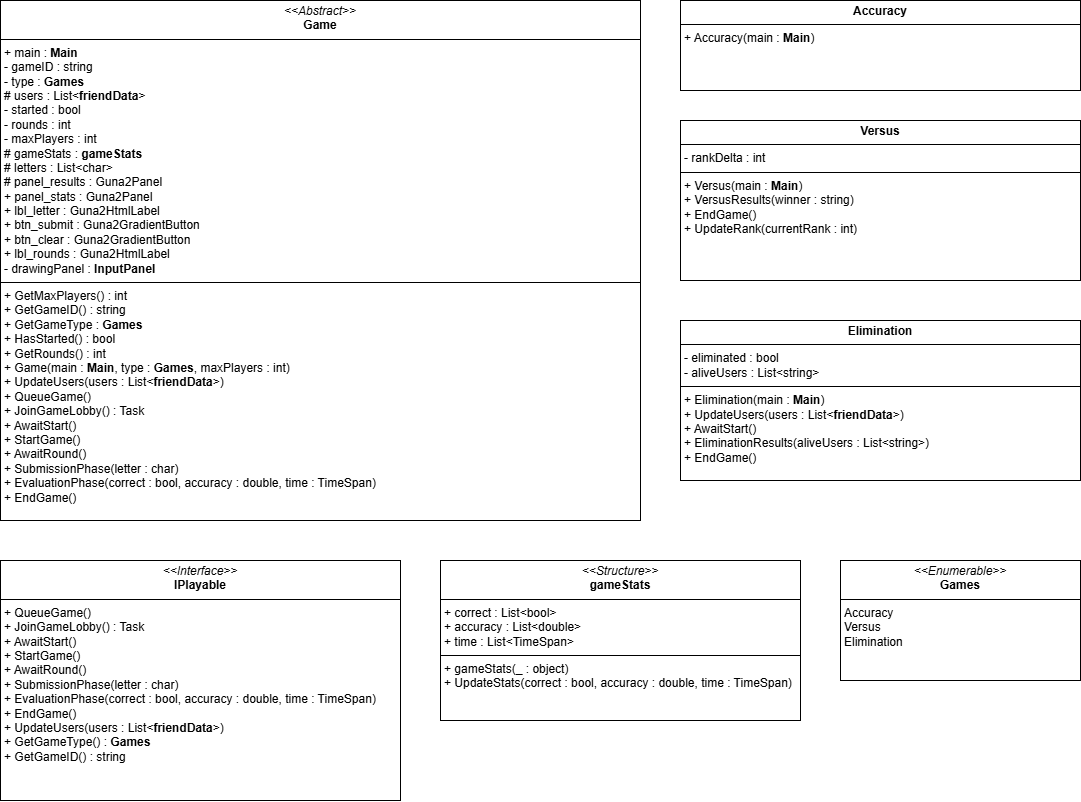
\includegraphics[width=1\linewidth]{resx/cgames_class.png}
    \caption{UML diagrams for the Game classes}
\end{figure}

\subsection{UI Design}

Each sub-menu within the client application draws its form controls onto a base layout which is configured in the constructor for the \textbf{Main} class. The majority of user interface updates are processed by the static \textbf{UXelements} class. The main menu, profile page, and game screens all draw their controls onto the form created by the \textbf{Main} class by passing the class instance as a parameter in the class constructors. \\

The `InitialiseComponent()' method of the \textbf{UXelements} class configures the base layout for the application. This includes the main panels which divide up the form, along with the `Close' and `Home' buttons. The form border style is set to `none', since a custom title bar is implemented instead which also prevents the user from dragging and resizing the window. Windows Forms has a tendency to break its controls on window resize events. \\

\begin{figure}[H]
    \centering
    
\includegraphics[width=0.75\linewidth]{resx/ui_layout.png}
    \caption{Layout for the base user interface}
\end{figure}

The main panels consist of a left, centre, and right panel. The left panel is divided into a smaller top panel and main bottom panel, which contains the `Home' button. The title bar sits above these panels and contains the `Close' button. \\

The click event handler for the `Home' button is attached in the `ResetLayout()' method. This cause the page text to be updated to ``Home'' and the `dequeueGame()' method to be invoked on the server if the user is in-game. The `profile' and `game' attributes of the `menu' structure are then disposed, and the `InitialiseComponent()' method is called. \\

The click event handler for the `Close' button is attached as part of configuring the base layout. This hides the form and invokes the `dequeueGame()' method on the server if the user is in-game. The `clientDisconnected()' method is then invoked, before closing the form.

\subsubsection{Accounts Page}

The accounts page is the first menu which the user is presented with when the application starts. The `username' and `password' text boxes can be edited, which the user can use to enter their login credentials. They can also create an account by clicking the `Create Account'  button. The language button in the bottom left of the form cycles through the available languages when it is clicked. The text in the form controls is immediately updated to reflect the new language selected. \\

A status indicator in the top left of the form informs the user of the state of the connection to the server. When the client successfully connects to the server, the loading animation stops and the label is set to `Connected'. If the connection fails, then the client will attempt to reconnect up to three times before disconnecting.

\begin{figure}[H]
    \centering
    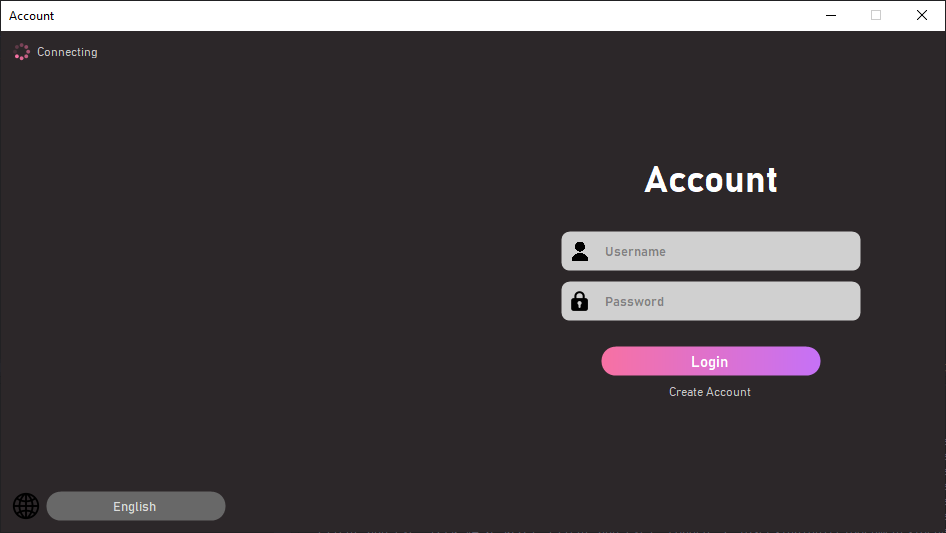
\includegraphics[width=0.75\linewidth]{resx/ui_accounts.png}
    \caption{Design for the Accounts form}
\end{figure}

If the user chooses to create an account, a `confirm password' text box is added where the user must enter their desired password twice in order to create an account. The `Login' button is replaced with the `Create Account' button, and the other controls are shifted around to accomodate the extra text box.

\begin{figure}[H]
    \centering
    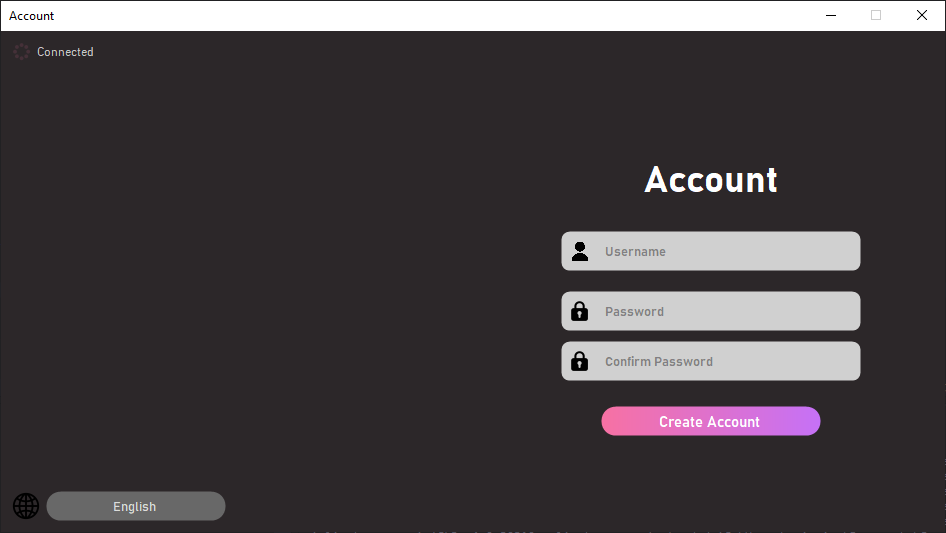
\includegraphics[width=0.75\linewidth]{resx/ui_accounts2.png}
    \caption{Design for the Accounts form}
\end{figure}

\subsubsection{Home Page}

The main panel on the home page lists the three available game to the user with a brief description and the ability to queue for each game. The left panel contains a list of the user's friends, seperated into whether they are online or offline. The right panel contains an overview of the user's statistics, as well as the `Profile' and `Edit' buttons. \\

The `Profile' button is used to access the profile page of the user. The click event handler for the button intialises a new instance of the \textbf{Profile} class with the user's userData.

\paragraph{Profile Updates\\}
The `Edit' button is used to customise the user's `about me' and change the language of the client application. The click event handler for the button creates a new \textbf{UpdateForm} dialog form. If the user clicks the `Confirm' button, then the `about me' and language which the user set are extracted using the appropriate methods of the form class. The `updateUserData()' method is then invoked on the server, passing the userID and updated `about me' and localisation.

\begin{figure}[H]
    \centering
    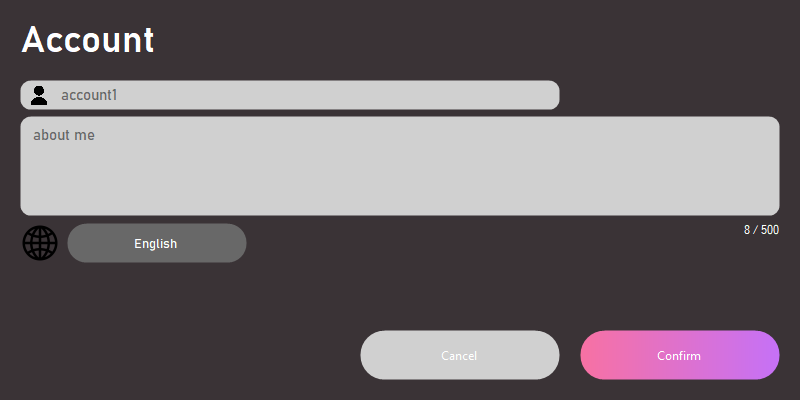
\includegraphics[width=0.75\linewidth]{resx/ui_edit.png}
    \caption{Design for the Edit Profile form}
\end{figure}

\paragraph{Menu Label\\}
The `page text' is a label in the top section of the left panel. It displays to the user what menu they are currently in, and is updated using the `UpdatePageText()' method which takes in a string as a parameter. This clears the panel and creates a new label, which it applies the passed string to its `text' property after translating it. \\

\paragraph{Friends\\}

The friends panel is added to the left panel and lists the user's friends seperated into online and offline. The `ConfigFriendsPanel()' method of the \textbf{Main} class seperates the user's friends into two lists based on whether they are online or offline. The `Online' label is created, withe the length of its respective list added to its right. The online users are then listed using a loop which increments the Y-position of the next label each iteration. The name of each button is mapped to the userID of the friend. This allows the click event handler to use the button's name to call the asynchronous `RequestProfile()' method, passing the userID of the friend as a parameter. This is then repeated for the offline users, with the Y-position incremented such that the offline users are places below all the online users. \\

The `RequestProfile()' method invokes the `requestProfile()' method on the server which returns a `userData' structure. A new \textbf{Profile} class is then instantiated with the returned userData as an argument to the constructor.

\paragraph{Statistics\\}

The right panel contains an overview of the user's account details, along with the options to view their profile and customise their `about me' and localisation. The summary of the statistics is created as a seperate panel which is then placed onto the right panel by the `ConfigStatsPanel()' method of the static \textbf{UXelements} class. \\

The values for the rank, total, and average accuracy are obtained from the static `CalculateStatsOverview()' method from the \textbf{Main} class. Local methods are used to reduce the volume of repeated code, and typically take arguments of position and size. 

\subsubsection{Profile}

The \textbf{Profile} form class is instantiated to display the statistics of a user for each letter. It contains private attributes of the `userData' structure for the requested user, and the instance of the \textbf{Main} class. The constructor for the class assigns values to these attributes and configures the form controls. A new panel is created to store each of the letters in, and the `ConfigStats()' method iterates through each letter and creates the appropriate controls. 

\begin{figure}[H]
    \centering
    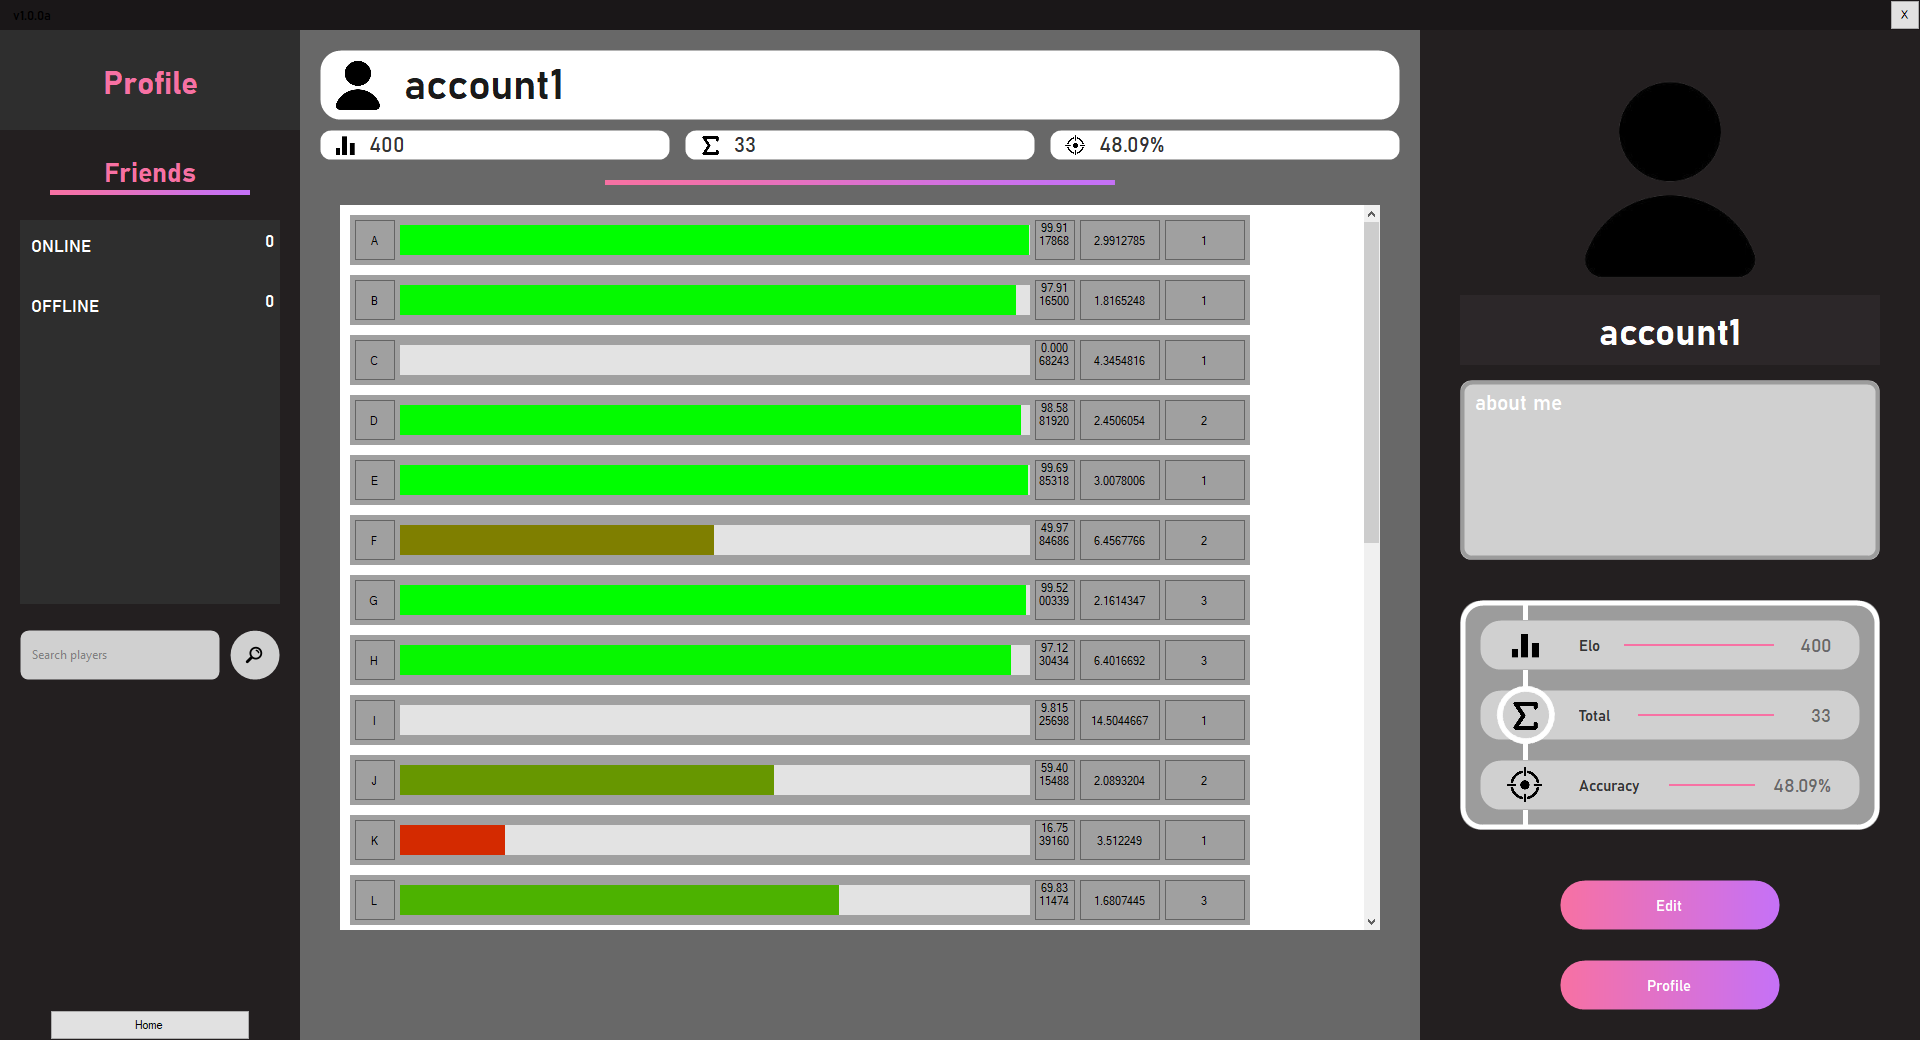
\includegraphics[width=0.75\linewidth]{resx/ui_profile.png}
    \caption{Design for the Profile page}
\end{figure}

\subsubsection{Games}
\paragraph{Drawing Panel\\}

The drawing panel is contained within a seperate class \textbf{InputPanel} which is intialised by the `ConfigGamePanel()' method of the \textbf{UXelements} class, and returned to the abstract \textbf{Game} class in the `AwaitRound()' method. The constructor for the \textbf{InputPanel} class takes as parameters the panel which the drawing panel is to be added to, and its position and size. The `LoadPanel()' and `ClearPanel()' methods are then called. \\

The `LoadPanel()' method creates a new Panel object and adds it to the controls of the base panel. A Bitmap object with identifier `drawing' is created by using the `CreateGraphics()' method of the Panel class. The `ClearPanel()' method uses the `Graphics' class to set all the pixels of the `drawing' Bitmap to white. This is then updated to the panel using the `DrawImageUnscaled()' method. \\

The class also contains event handlers for the state of the left mouse button and the movement of the mouse cursor in the panel. The mouse down event handler sets the boolean value `draw' to true and sets the position of the pen to the mouse position. The mouse up event handler sets the boolean value `draw' to false. \\

The mouse move event handler sets the position of the pen to the position of the mouse cursor. If the boolean value `draw' is true, then a new `Graphics' object is created from the `drawing' Bitmap. A new `Pen' object is created with the set pen thickness and colour, and the `DrawLine()' of the Panel class draws a line using the `Pen' object from the previous position of the mouse to its current position. This is then rendered onto the Panel using the `DrawImageUnscaled()' method.

\begin{figure}[H]
    \centering
    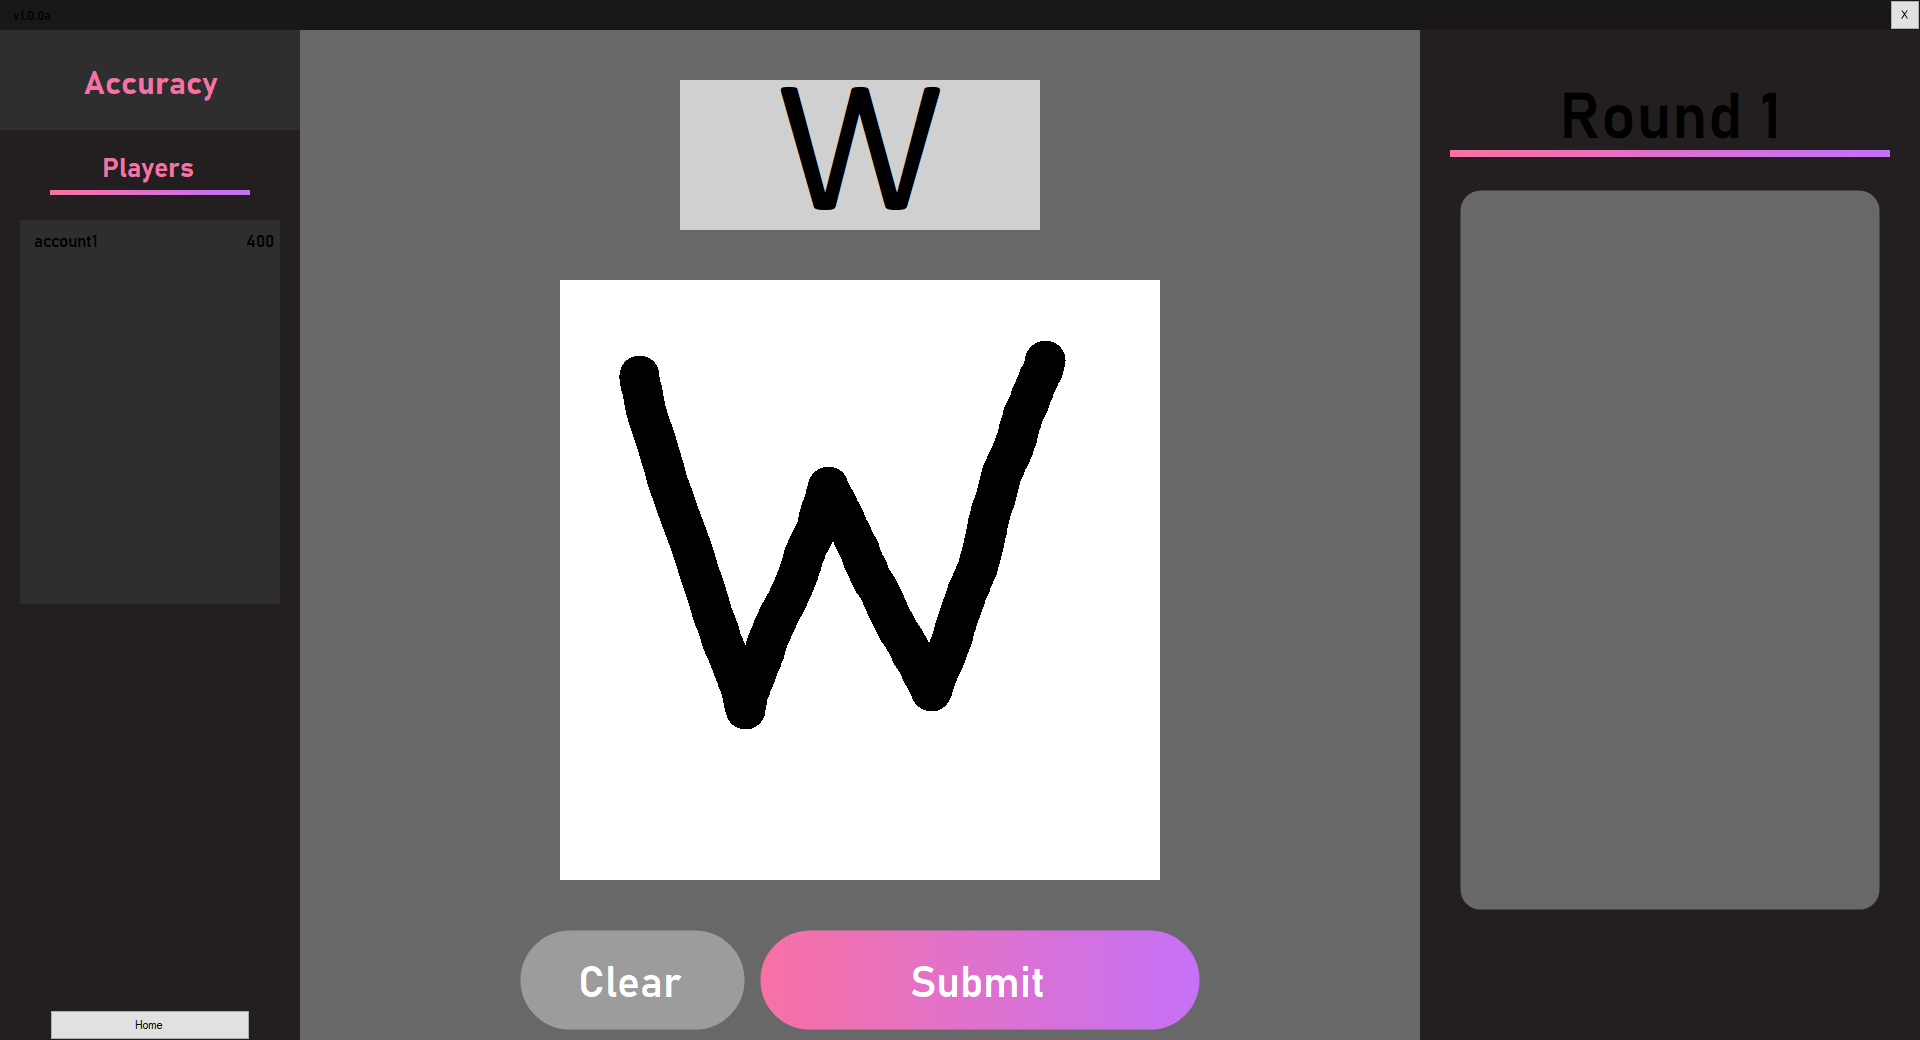
\includegraphics[width=0.75\linewidth]{resx/ui_drawing.png}
    \caption{Design for the drawing panel}
\end{figure}

\paragraph{Results\\}

The results panel is configured by the `ConfigResultsPanel()' method of the \textbf{UXelements} class which returns the created panel. This allows for the `Versus' and `Elimination' game types to access the panel and add the controls for the extra information regarding these gamemodes to the panel once the server has sent the data. \\

The panel contains the letter of the current round as well as the user's results for their submission: accuracy, time, and if it was correct. `Deltas' are also presented to the user, which represent the difference between their submission and their average for that letter. These are calculated by subtracting the accuracy and time of the submission from the values stored in the `statistics' attribute of the userData. The colour of the accuracy `delta' is set to red if the accuracy of the submission is less than the average for the letter, and green otherwise. The colour of the time `delta' is set to green if the time of the submission is less than ther average for the letter, and red otherwise. \\

This does result in `fake' deltas being calculated if it is the first time which the user has been given the current letter, since the values in their userData will be zero. While this isn't a common issue, it could be something that confuses some users. \\

A progress bar is also created for the accuracy, where the bar is appropriately set to fill the same percentage of space as the accuracy of the submission. The accuracy value is also displayed on the right side of the bar. The time elapsed for the submission is placed inside a similar progress bar, however its value is always set to 0\%, since the time cannot be objectively placed somewhere on a scale.

\begin{figure}[H]
    \centering
    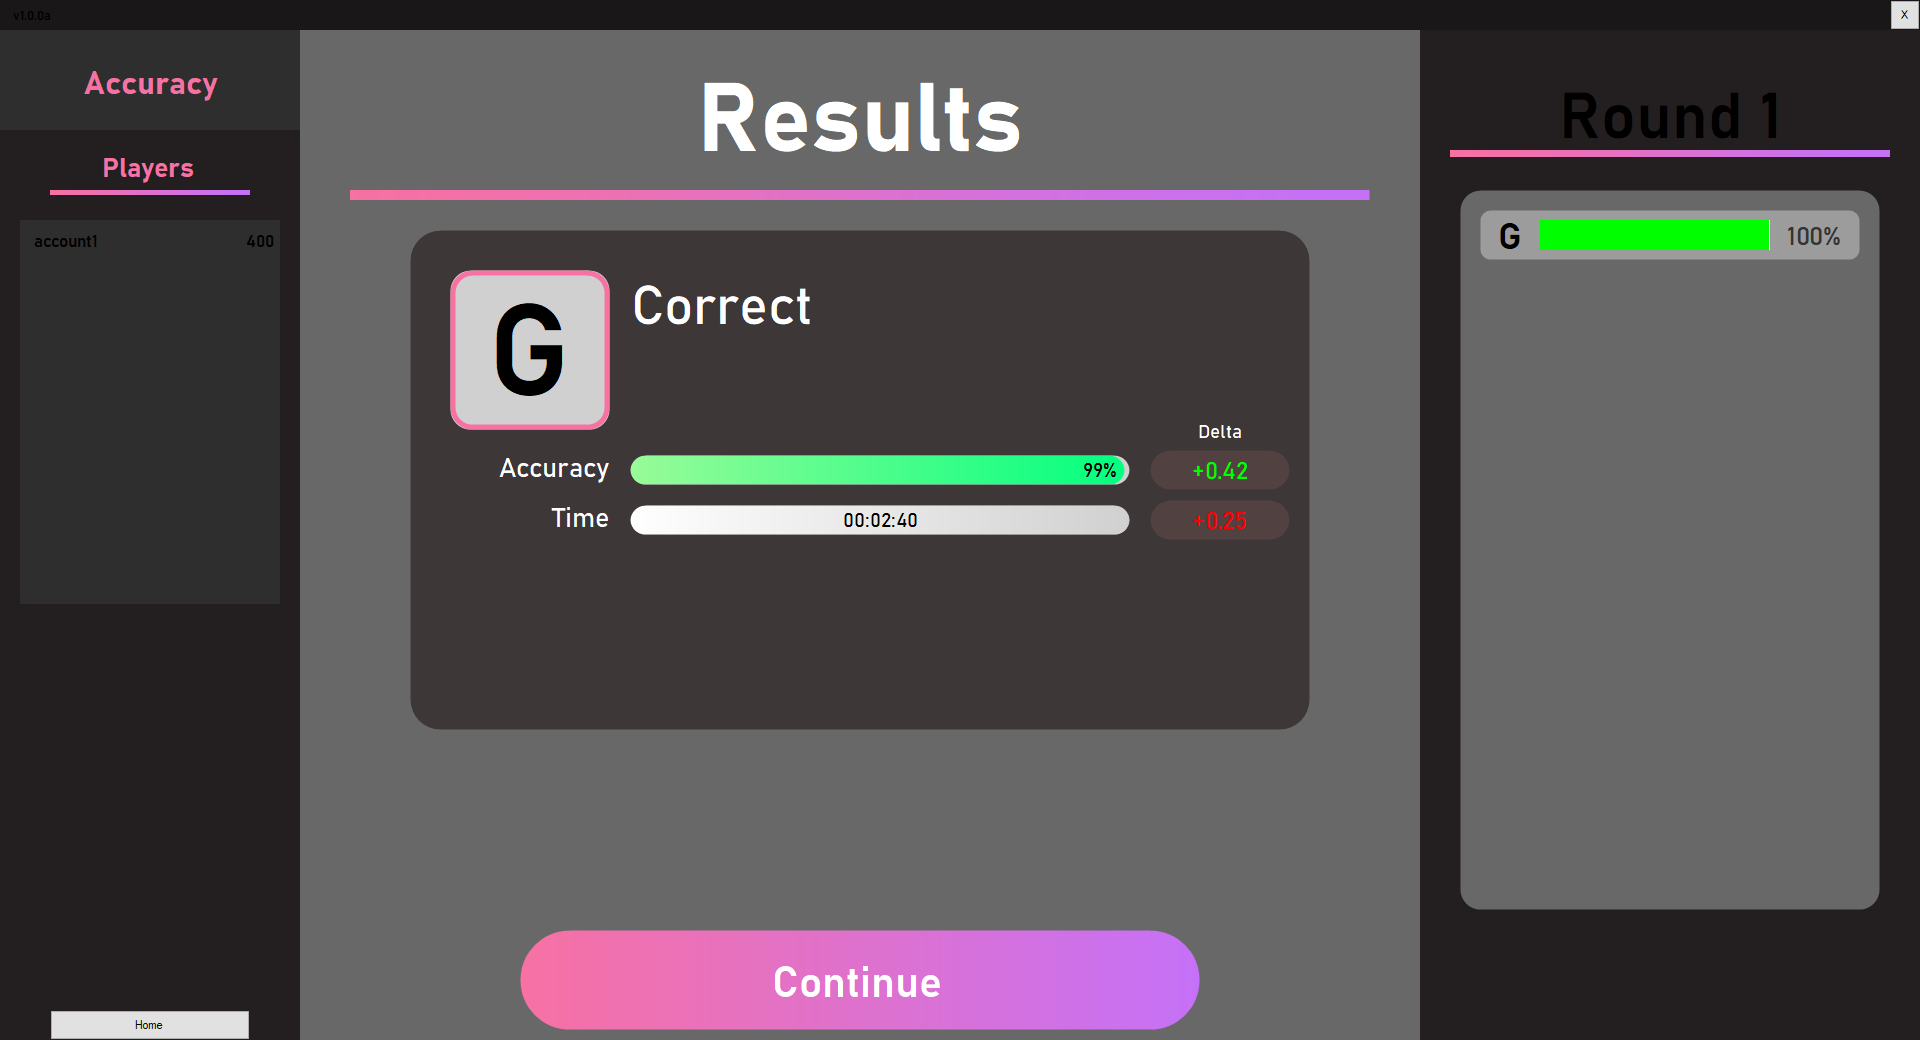
\includegraphics[width=0.75\linewidth]{resx/ui_resacc.png}
    \caption{Design for the results panel in the `Accuracy' game type}
\end{figure}

\begin{figure}[H]
    \centering
    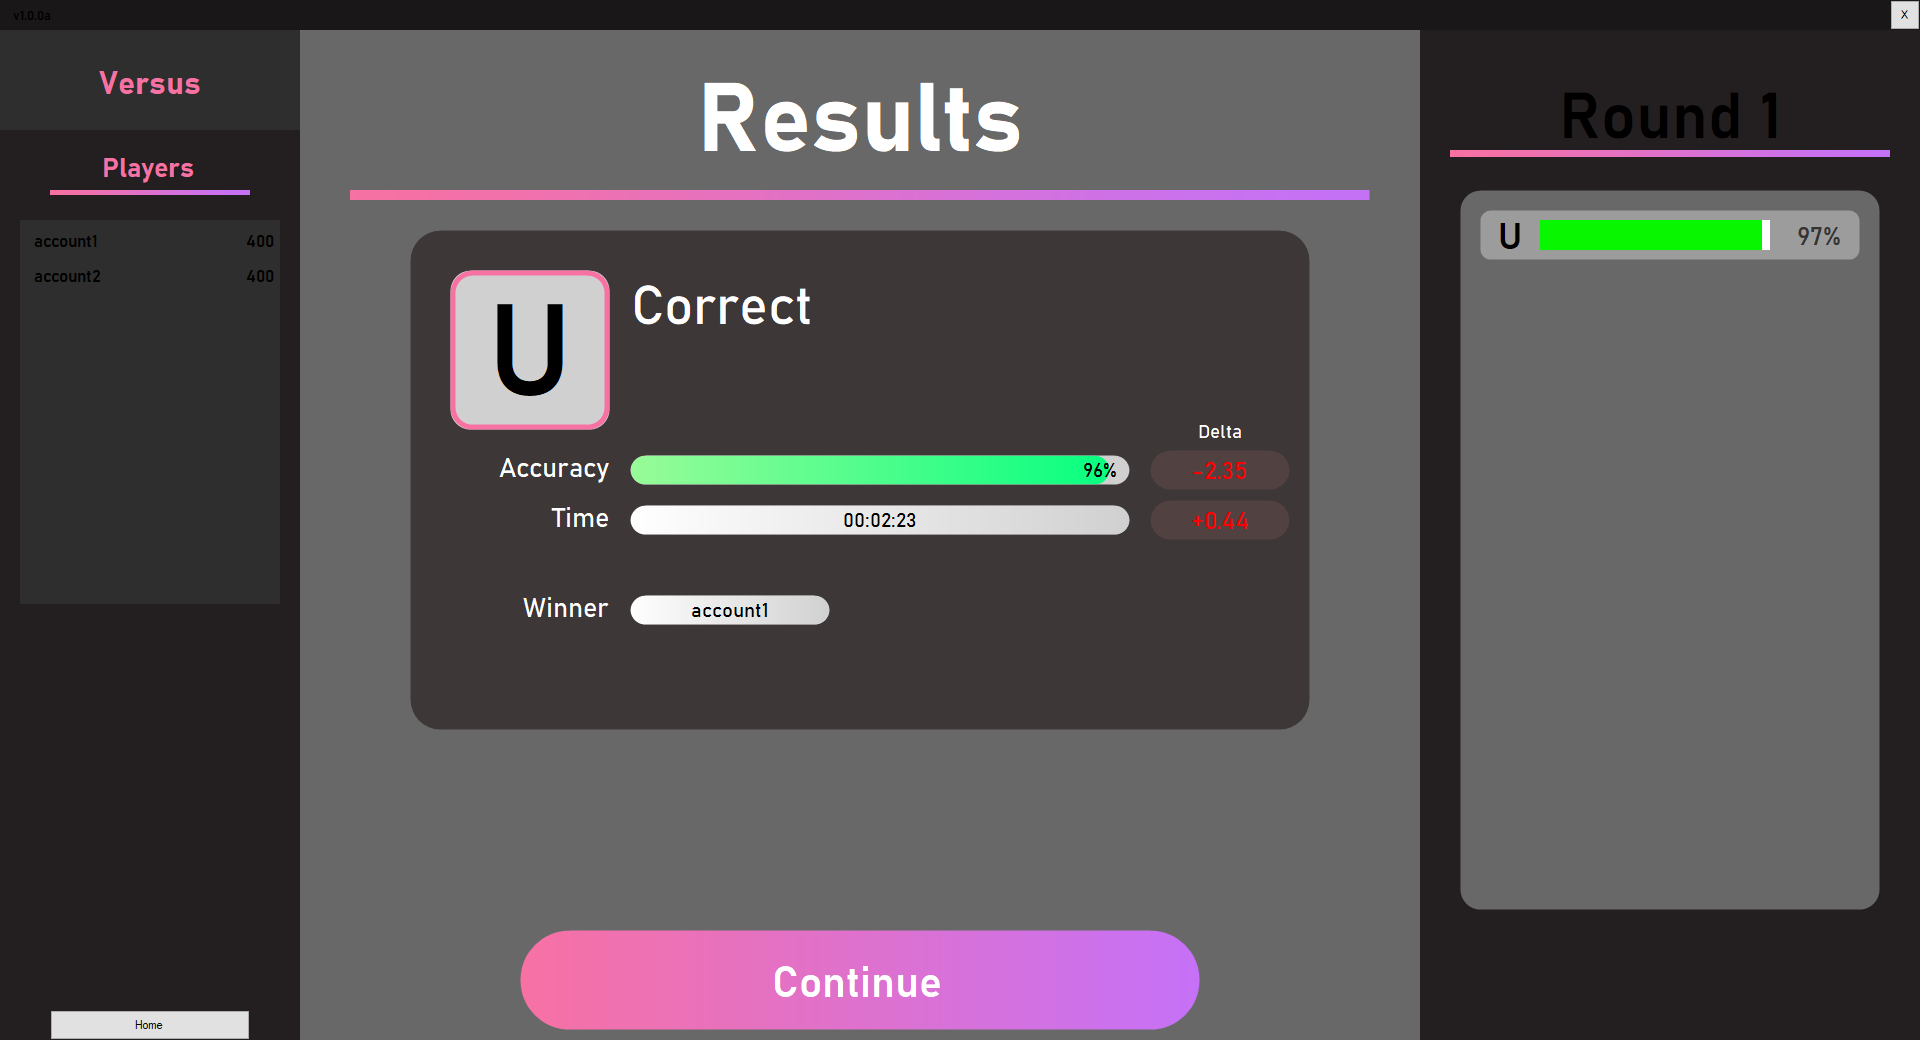
\includegraphics[width=0.75\linewidth]{resx/ui_resver.png}
    \caption{Design for the results panel in the `Versus' game type}
\end{figure}

\begin{figure}[H]
    \centering
    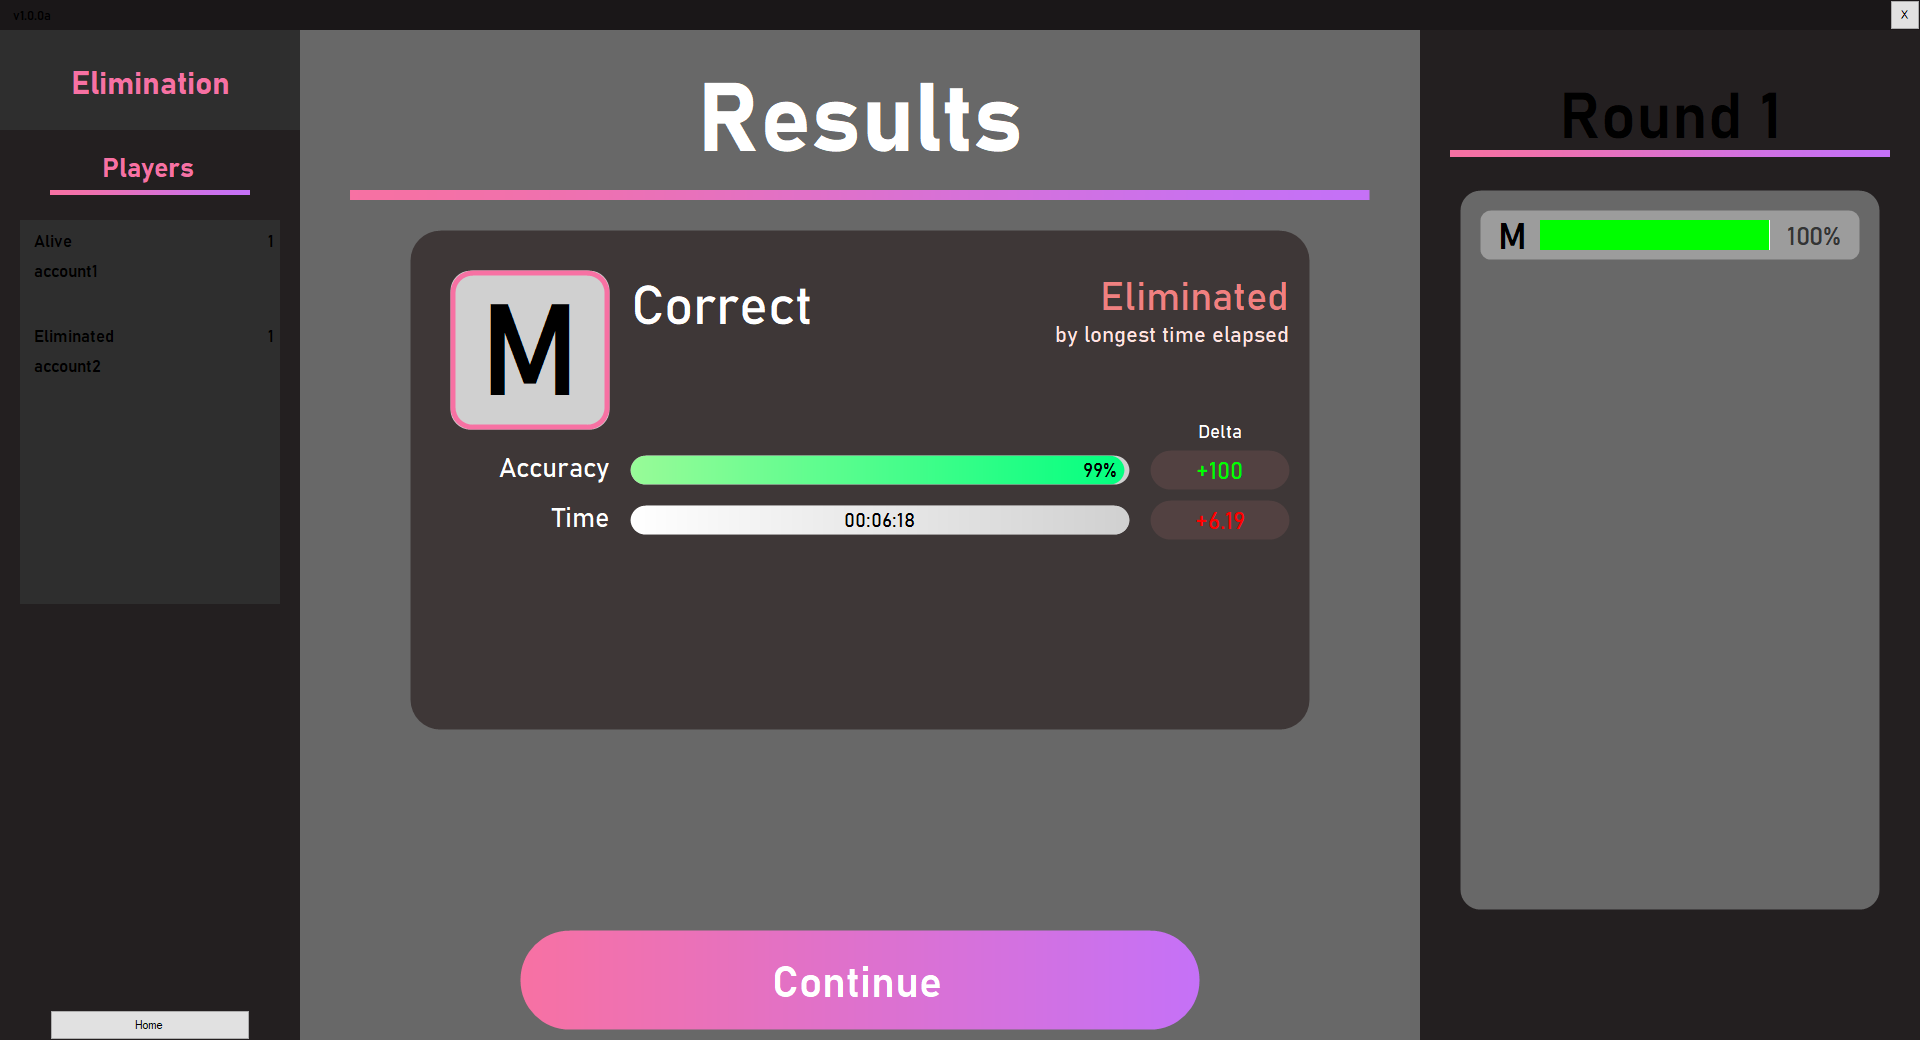
\includegraphics[width=0.75\linewidth]{resx/ui_reseli.png}
    \caption{Design for the results panel in the `Elimination' game type}
\end{figure}


\subsection{Object-Oriented Design}
\subsubsection{Class Diagrams}

The dependencies between classes has not been shown in the diagram below as it severely impacts the legibility. Static classes have been denoted by underlining the class identifier. While the \textbf{Form} class not accessed by any classes directly, I chose to include it in order to show which classes derive and use Windows Forms controls.

% // missed language class and hub_connection is static
\begin{figure}[H]
    \centering
    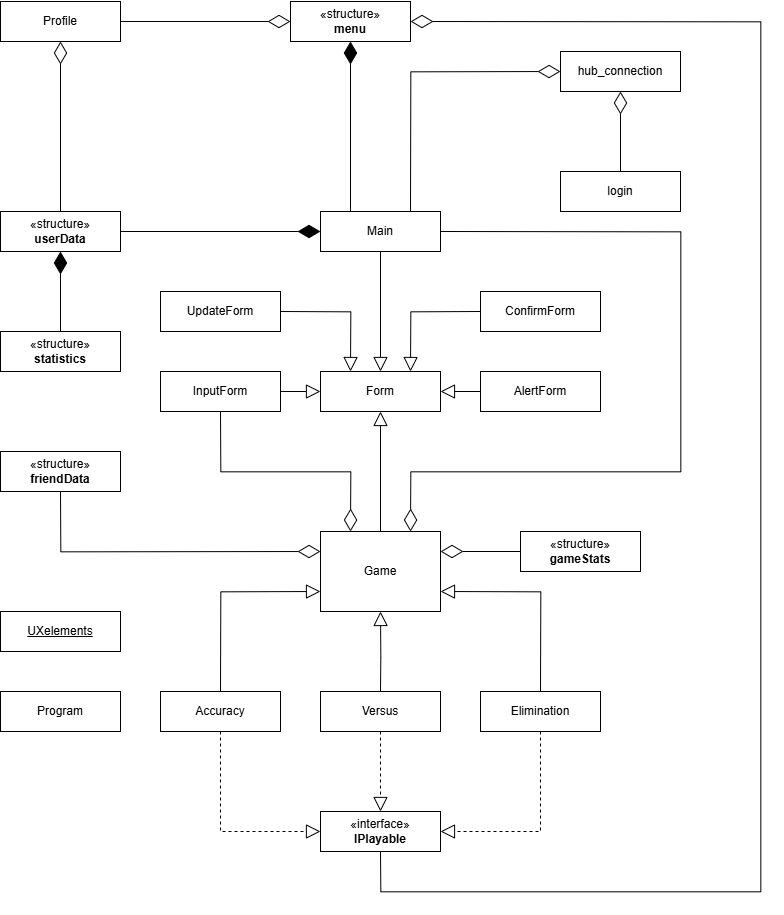
\includegraphics[width=1\linewidth]{resx/client-class-overview.png}
    \caption{Relationships between the client classes}
\end{figure}

\subsection{Client-Server Connection}

The client handles its connection to the server using a `HubConnection' object, which can invoke methods on the server and set up handlers to manage incoming invokations. Both the \textbf{Login} class and the \textbf{Main} class contain their own `HubConnection' object, to seperate the handlers for a user who is logged in and a user who is not. \\

\subsubsection{Creating a Connection}

The \textbf{hub\_connection} class contains the `ConfigConnection()' method which creates a new `HubConnection' object. The method initialises a new `HubConnectionBuilder', which the address of the server is attached to. The `Build()' method of this object is then called which returns a `HubConnection' object.

\subsubsection{Connection Handlers}

The connection handlers are added by the `AddHandles()' method for the \textbf{Main} class, and the `AddLoginHandles()' for the \textbf{Login} class. Since these are called asynchronously, the majority of the handles execute by invoking the instance of the \textbf{Main} class. This is a method of the \textbf{Form} class which allows controls to be accessed from a thread which they were not created on. The `Invoke()' method takes in an Action as a parameter which is set to the appropriate method in the \textbf{Main} class for the current handler.

\begin{minted}{csharp}
    connection.On<userData>("receiveUserData", (userData) =>
    {
        main.Invoke(new Action(() => main.ClientConnected(userData)));
    });
\end{minted}

\subsubsection{Starting a Connection}

The connection is started by the `StartConnection()' method, which takes in the `HubConnection' object as a parameter. The number of retries is initially set to -1 since the first attempt at connection is not a retry. A while loop is then started which runs until the connection state is not `Disconnected'. The number of retries is incremented by one, and a check is made to see if it exceeds three retries. If this is the case then the connection status label displays ``Disconnected'' and the while loop is broken. Otherwise, the connection is attempted to be started and the information label is reset. If an exception is thrown such that the client failed to connect to the server, the information label displays an error.

\subsubsection{Handling Connection Loss}

Before a request is made to the server, a check is always made to confirm that the connection state is `Connected'. If this is not the case, then the `PerfomClick()' method of the `Home' button is called to return the user to the home screen. The client application may not immediately recognise a loss of connection when it occurs, and the user interacting with any controls which communicate with the server may cause unexpected behaviour. \\

When it is detected that the connection has been lost, the `ConnectionClose()' method is called which attempts to return to the home screen. A new alert form is then configured to inform the user of the loss of connection and that the application will be restarted. This is because a disconnection may cause unexpected behaviour on the server regarding the user's ConnectionID, so it is safer to restart and reset the user's ConnectionID.\@ Any attempt to interact with the form controls in this method is wrapped in a try-catch block, since the exact state of the client application is unknown. \\ 

\newpage
\section{Testing}
\noindent\rule{\textwidth}{0.2pt}
\renewcommand{\arraystretch}{1.5} % 1.5x default spacing

% Custom column types for tabularx
\newcolumntype{L}{>{\raggedright\arraybackslash\nohyphens}X}
\newcolumntype{C}{>{\centering\arraybackslash\nohyphens}X}
\newcolumntype{R}{>{\raggedleft\arraybackslash\nohyphens}X}

\subsection{Testing}

The layout for the testing section first outlines the tests that will be completed, along with any information regarding these tests---such as the software used or any changes to the system. The tests are then given in a list, with each test having a timestamp in bold which links the test to the appropriate section in the testing video. If the test is directly testing one of the objectives, then this has been given in square brackets after the timestamp. If there is no link to an objective, then it is testing for the robustness of the solution. A table then outlines the input used to set up each test, along with the expected and observed outcomes. \\

\href{https://www.google.com}{Link to the Testing Video}

\subsubsection{Accounts}

\begin{enumerate}

    \item \textbf{Logging in to an account}
    
    These tests involve the login process to an existing account: `account1' which was setup prior to these tests. For each test, the input is entered into the `Username' and `Password' text boxes, and the `Login' button is clicked. The output is typically given by a red message beneath the `Password' text box.
    
    \begin{enumerate}
        \item \textbf{00:00} [1.a.i] Entering an unregistered username returns a suitable error message.
        \item \textbf{00:04} [1.a.i] Access is denied when entering an incorrect password for an existing account.
        \item \textbf{00:09} [1.a.i] A login request is not made to the server if any fields are left blank.
        \item \textbf{00:12} [1.a.ii] Entering valid credentials causes the main application to load for the user.
     \end{enumerate}

    \begin{table}[H]
    \centering
        \begin{tabularx}{\textwidth}{|L|L|L|}
        \hline
        \textbf{Input} & \textbf{Expected outcome} & \textbf{Observed outcome} \\\hline
        ``account2'' and ``password'' & ``User does not exist'' & ``User does not exist'' \\\hline
        ``account1'' and ``wrongpassword'' & ``Incorrect password'' & ``Incorrect password'' \\\hline
        Leaving one or more fields blank & Login request is not made & Login request is not made \\\hline
        ``account1'' and ``password'' & Main application loads & Main application loads \\\hline
        \end{tabularx}
    \end{table}

    4/4 tests passed. \\

    \item \textbf{Creating an account}
    
    For each test, the input is entered into the `Username' and both `Password' text boxes, followed by the user clicking the `Create Account' button. Unless stated otherwise, the input into both `Password' text boxes is identical.

    \begin{enumerate}
        \item \textbf{00:18} [1.b.ii] Entering a username which is already registered returns a suitable error message.
        \item \textbf{00:26} [1.b.i]An account request is not made to the server if any fields are left blank.
        \item \textbf{00:29} [1.b.i] An account request is not made to the server if the passwords do not match.
        \item \textbf{00:36} [1.b.iii] Entering valid credentials causes the main application to load for the new user.
        \begin{enumerate}
            \item \textbf{00:40} [5.d.ii] A new account is created in the database with a hashed password.
            \item \textbf{00:46} [1.b.iii] Empty statistics are created for the letters A-Z in the database.
        \end{enumerate}
    \end{enumerate}

    \begin{table}[H]
    \centering
        \begin{tabularx}{\textwidth}{|L|L|L|}
        \hline
        \textbf{Input} & \textbf{Expected outcome} & \textbf{Observed outcome} \\\hline
        ``account1'' with ``password'' & ``Username is not available'' & ``Username is not available'' \\\hline
        Leaving one or more fields blank & Login request is not made & Login request is not made \\\hline
        ``account2'' with ``pass'' and ``password'' & ``Passwords do not match'' & ``Passwords do not match'' \\\hline
        ``account2'' and ``password'' & Main application loads & Main application loads \\\cline{2-3}
        & Entry added in `userData' table with a hashed password & Entry added in `userData' table with a hashed password \\\cline{2-3}
        & Empty statistics for letters A-Z created in `statistics' table & Empty statistics for letters A-Z created in `statistics' table \\\hline
        \end{tabularx}
    \end{table}

    6/6 tests passed. \\

    \item \textbf{Localisation and Other}

    \begin{enumerate}
        \item \textbf{00:54} [1.c] The language chosen is applied to the main application which loads with this langauge set.
        \item \textbf{01:05} [1.c] The language chosen is saved to the user's account data in the database.
        \item \textbf{01:24} A user cannot login twice on two different instances of the client application.
    \end{enumerate}

    \begin{table}[H]
    \centering
        \begin{tabularx}{\textwidth}{|L|L|L|}
        \hline
        \textbf{Input} & \textbf{Expected outcome} & \textbf{Observed outcome} \\\hline
        Choosing `Français' as the language & Main application uses the French language & Main application uses the French language \\\cline{2-3}
        & Localisation is set to `fr' in the database & Localisation is set to `fr' in the database \\\hline
        Logging in while the account is logged in on a different instance & ``User is logged in on another device'' & ``User is logged in on another device'' \\\hline
        \end{tabularx}
    \end{table}

    3/3 tests passed. \\

\end{enumerate}

\subsubsection{Games}

\begin{enumerate}

    \item \textbf{Features of a generic game}

    An `Elimination' game may have more than 10 rounds, however this requires considerable setup beforehand. Instead I have changed the number of rounds of the `Accuracy' game type to 20 for these tests only, since both game types use the same method to configure the right panel. \\
    
    Obtaining an exact value for the elapsed time of a letter is not feasible, however it can be approximated with a timer. Some error in this measurement is expected due to server latency and human reaction time, however it should be sufficient to test the recorded time. In order to improve the accuracy of starting and stopping the timer, I set up a keybind to start and stop the timer. This allowed me to press the keybind with the `Continue' and `Submit' buttons at very similar times. After clicking `Continue' there is a 3 second wait before the server timer starts and the letter is shown to the client. Therefore I will be comparing the time recorded by LiveSplit against the returned time with 3 seconds added to it.
    
    \begin{enumerate}
        \item \textbf{02:10} [2.e] The list of users currently in a game is updated when a user joins or leaves the game.
        \item \textbf{02:15} [2.b] A range of characters from the Latin alphabet are presented to the user.
        \item \textbf{02:50} The time displayed in the results is close in value to the actual elapsed time.
        \item \textbf{02:59} [2.g] The next round starts when all users have clicked the `Continue' button.
        \item \textbf{03:38} [2.c.i] The drawing panel can be cleared.
        \item \textbf{03:07} [2.f] Only the results of the last 10 rounds are displayed on the right panel.
    \end{enumerate}

    \begin{table}[H]
    \centering
        \begin{tabularx}{\textwidth}{|L|L|L|}
        \hline
        \textbf{Input} & \textbf{Expected outcome} & \textbf{Observed outcome} \\\hline
        Leaving a game as `account2' with `account1' present & The list of users for a user in the game is updated & `account2' is removed from the list \\\hline
        Playing 5 rounds of the `Accuracy' game type & There is variation in the letters presented & There is variation in the letters presented \\\hline
        Timing the elapsed time drawing a letter using LiveSplit & Returned time is within 5\% of the recorded time of 2.29 seconds & Returned time is 2.28 seconds which is within 0.4\% \\\hline
        Clicking `Continue' on all client applications & Next round starts when all users have clicked `Continue' & Next round starts when all users have clicked `Continue' \\\hline
        Drawing a letter and clicking the `Clear' button & The drawing panel is cleared & The drawing panel is cleared \\\hline
        Playing 11 rounds in the `Accuracy' game type & Only the 10 most recent results are shown & Only the 10 most recent results are shown \\\hline
        \end{tabularx}
    \end{table}

    6/6 tests passed. \\

    \item \textbf{Queueing for the `Accuracy' game type}

    \begin{enumerate}
        \item \textbf{01:30} [2.a] The `Accuracy' game type starts when it is full.
        \item \textbf{01:35} Queueing for the `Accuracy' game type always creates a new game.
    \end{enumerate}

    \begin{table}[H]
    \centering
        \begin{tabularx}{\textwidth}{|L|L|L|}
        \hline
        \textbf{Input} & \textbf{Expected outcome} & \textbf{Observed outcome} \\\hline
        Queueing for the `Accuracy' game type & The game starts immediately & The game starts immediately \\\hline
        Queueing multiple users for the `Accuracy' game type & Each user is queued into a different game & Each user is queued into a different game \\\hline
        \end{tabularx}
    \end{table}

    1/1 test passed. \\
    
    \item \textbf{Queueing for the `Versus' game type}
    
    \begin{enumerate}
        \item \textbf{01:44} [2.a] The `Versus' game type starts when two users are queued for it.
        \item \textbf{01:39} [2.a] The `Versus' game does not start if there are less than 2 users in the lobby.
        \item \textbf{01:50} A third user who queues for the `Versus' game type is queued into a new game.
    \end{enumerate}

    \begin{table}[H]
    \centering
        \begin{tabularx}{\textwidth}{|L|L|L|}
        \hline
        \textbf{Input} & \textbf{Expected outcome} & \textbf{Observed outcome} \\\hline
        Queuing two user into `Versus' & The game starts & The game starts \\\hline
        Queueing one user into `Versus' & The game does not start & The game does not start \\\hline
        Queueing three users into `Versus' & The third user is queued into a different game & The third user is queued into a different game \\\hline
        \end{tabularx}
    \end{table}

    3/3 tests passed. \\

    \item \textbf{Winning conditions for the `Versus' game type}
    
    \begin{enumerate}
        \item \textbf{04:08} [2.h.i.B] If one user is correct and the other user is incorrect, the user who is correct wins the round.
        \item \textbf{04:18} [2.h.i.B] If both users are correct, the user with the fastest time wins the round.
        \item \textbf{04:32} [2.h.i.B] If both users are incorrect, then it is a draw and neither user wins the round. 
    \end{enumerate}

    \begin{table}[H]
    \centering
        \begin{tabularx}{\textwidth}{|L|L|L|}
        \hline
        \textbf{Input} & \textbf{Expected outcome} & \textbf{Observed outcome} \\\hline
        Drawing the correct letter for one user, and an incorrect letter for the other user & The correct user wins the round & The correct user wins the round \\\hline
        Drawing the correct letter for both users & The user with the fastest time wins the round & The user with the fastest time wins the round \\\hline
        Drawing an incorrect letter for both users & Neither user wins the round & Neither user wins the round \\\hline
        \end{tabularx}
    \end{table}

    3/3 tests passed. \\

    \item \textbf{Elo Formulae}

    For this test, two accounts are setup with a given Elo rating where `account1' has a rating of 400, and `account2' has a rating of 300. A `Versus' game is then started with both of these users and `account1' is given 4 wins, 1 draw, and 5 losses. This results in `account1' obtaining a score of 4.5, and `account2' obtaining a score of 5.5. The expected scores of each user are then calculated using the Elo rating of each user.
    
    \begin{equation*}
        E_A=10\cdot \frac{1}{1+10^{(300---400) / 400}}\approx 6.400649998
    \end{equation*}
    \begin{equation*}
        E_B=10\cdot \frac{1}{1+10^{(400---300) / 400}}\approx 3.599350002
    \end{equation*}

    The updated ranks for both users can then be calculated using their expected score and their actual score.
    
    \begin{equation*}
        R'_A=400+\frac{32}{10}\cdot (4.5-6.400649998)=393.91792\approx 393
    \end{equation*}
    \begin{equation*}
        R'_B=300+\frac{32}{10}\cdot (5.5-3.599350002)=306.08208\approx 306
    \end{equation*}

    \begin{enumerate}
        \item \textbf{04:45} [2.h.i.A] [3.c.i] The Elo rating for users in a `Versus' game is updated correctly at the end of the game.
    \end{enumerate}

    \begin{table}[H]
    \centering
        \begin{tabularx}{\textwidth}{|L|L|L|}
        \hline
        \textbf{Input} & \textbf{Expected outcome} & \textbf{Observed outcome} \\\hline
        `account1' gaining a score of 4.5 and `account2' gaining a score of 5.5 & The rating of the users changes to 393 and 306 respectively &  `account1' changes to 393 and `account2' changes to 306 \\\hline
        \end{tabularx}
    \end{table}

    1/1 test passed. \\

    \item \textbf{Queueing for the `Elimination' game type}
    
    These tests for the `Elimination' game type involve start conditions. It should be noted that the number of players to start this game type was set to 3 instead of 12, in order to make testing more convenient.

    \begin{enumerate}
        \item \textbf{02:05}[2.a] The `Elimination' game type starts when the appropriate number of users are queued for it.
        \item \textbf{01:56} [2.a] The `Elimination' game type does not start if it has less users than required to start the game.
    \end{enumerate}

    \begin{table}[H]
    \centering
        \begin{tabularx}{\textwidth}{|L|L|L|}
        \hline
        \textbf{Input} & \textbf{Expected outcome} & \textbf{Observed outcome} \\\hline
        Queueing 3 users for the `Elimination' game type & The game starts & The game starts \\\hline
        Queuing 2 users for the `Elimination' game type & The game does not start & The game does not start \\\hline
        \end{tabularx}
    \end{table}

    2/2 tests passed. \\

    \item \textbf{Winning conditions for the `Elimination' game type}
    
    The following tests involve the logic for a user passing a given round in the `Elimination' game type.

    \begin{enumerate}
        \item \textbf{05:13} [2.h.iii.A] If all of the users are correct, then the user with the longest elapsed time is eliminated.
        \item \textbf{05:28} [2.h.iii.A] If some of the users are incorrect, then these users only are eliminated.
        \item \textbf{05:41} [2.h.iii.A] If all of the users are incorrect, then none of the users are eliminated.
    \end{enumerate}

    \begin{table}[H]
    \centering
        \begin{tabularx}{\textwidth}{|L|L|L|}
        \hline
        \textbf{Input} & \textbf{Expected outcome} & \textbf{Observed outcome} \\\hline
        Drawing the correct letter for all users & The user with the longest elapsed time is eliminated & The user with the longest elapsed time is eliminated \\\hline
        Drawing an incorrect letter for the user `account3' & This user is eliminated while the other users move to the next round & `account3' is eliminated \\\hline
        Drawing an incorrect letter for all users & None of the users are eliminated & None of the users are eliminated \\\hline
        \end{tabularx}
    \end{table}

    3/3 tests passed. \\

    \item \textbf{Progression of the `Elimination' game type}
    
    The following tests expand on the game progressing when all users have clicked the `Continue' button. In the case of the `Elimination' game type, only the alive users are required to click this button for the game to progress, even though eliminated users are also given this button. In the case of the eliminated users, they are directed to the `Game End' screen. If there is only one alive user left, then the game has ended and that user has won.

    \begin{enumerate}
        \item \textbf{06:40} [2.h.iii.D] The next round in the `Elimination' game type occurs when all alive users have clicked `Continue'.
        \item \textbf{06:28} [2.h.iii.A] An eliminated user will be shown the `Game End' screen when clicking the `Continue' button.
        \item \textbf{06:49} [2.h.iii.C] An `Elimination' game will end when there is only one alive user.
    \end{enumerate}

    \begin{table}[H]
    \centering
        \begin{tabularx}{\textwidth}{|L|L|L|}
        \hline
        \textbf{Input} & \textbf{Expected outcome} & \textbf{Observed outcome} \\\hline
        Clicking `Continue' on an eliminated user, followed by all alive users & Next round will start after clicking `Continue' on all alive users & Next round starts after clicking `Continue' on all alive users \\\hline
        Clicking `Continue' on an eliminated user & The `Game End' screen is shown & The `Game End' screen is shown \\\hline
        A player winning with only 2 players alive & The `Game End' screen is shown for both users & The `Game End' screen is shown for both users \\\hline
        \end{tabularx}
    \end{table}

    3/3 tests passed. \\
    
\end{enumerate}

\subsubsection{Neural Network}

\begin{enumerate}
    \item \textbf{Evaluating user submissions}
    
    The following tests ensure the neural network is correctly evaluating a user's submission. These include tests for various orientations, positions, and obscure cases. The test for confirming that the neural network marks correct submissions with a high accuracy uses the same footage as showing that a range of Latin character are presented to the user.

    \begin{enumerate}
        \item \textbf{02:15} [5.c.ii] Drawing the correct letter is given a very high accuracy. % part of range of letters
        \item \textbf{03:19} [5.c.iii]Drawing the correct letter very small and in the corner is given a high accuracy.
        \item \textbf{03:47} Drawing the correct letter upside down.
        \item \textbf{03:25} [5.c.ii] Drawing the correct letter but malformed is given a medium accuracy.
        \item \textbf{03:43} [5.c.ii] Drawing an incorrect letter is given a low accuracy and marked as incorrect.
        \item \textbf{03:53} Filling the drawing panel in does not cause unexpected behaviour.
        \item \textbf{04:02} Leaving the drawing panel empty does not cause unexpected behaviour.
    \end{enumerate}

    \begin{table}[H]
    \centering
        \begin{tabularx}{\textwidth}{|L|L|L|}
        \hline
        \textbf{Input} & \textbf{Expected outcome} & \textbf{Observed outcome} \\\hline
        Accurately drawing the given letter in the drawing panel & The returned accuracy is high & The returned accuracy is high \\\hline
        Accuractely drawing the given letter in the corner of the panel with a smaller size & The returned accuracy is high & The returned accuracy is 99\% \\\hline
        Drawing the given letter upside down & The submission is marked as incorrect and given a low accuracy & The submission is marked as incorrect and given an accuracy of 0\% \\\hline
        Drawing a malformed version of the correct letter & The submission is marked as correct and given a medium accuracy & The submissions are marked as correct and given accuracies of 64\% and 60\% \\\hline
        Filling in the drawing panel & No unexpected behaviour occurs & No unexpected behaviour occurs \\\hline
        Leaving the drawing panel empty & No unexpected behaviour occurs & No unexpected behaviour occurs \\\hline
        \end{tabularx}
    \end{table}

    7/7 tests passed.

    \item \textbf{Training the neural network}
    
    The following tests confirm that the neural network is correctly applying the backpropagation algorithm to the training data. The previous sets of tests show that the network is sufficiently trained therefore it is likely these tests will also pass. Regardless, these tests are still necessary for completeness. The randomness of the training data has been temporarily removed for these tests, and additional console logs have been added.

    \begin{enumerate}
        \item \textbf{05:52} The neuron errors for the output layer are correctly calculated.
        \item \textbf{06:02} The neuron errors for the hidden layers are correctly calculated.
        \item \textbf{06:08} The network shows significant statistical evidence of correctly selecting the drawn letter.
    \end{enumerate}

    The neuron error for the output layer is calculated using the activated values of the neurons. Using a breakpoint in the program, I have determined the activated value of the `K' neuron to be approximately 0.00199. The value of \(y\) is 0, since the expected forward pass would have 0\% confidence that the `N' in the image is a `K'.

    \begin{equation*}
        \delta = 2\cdot (0.00199---0) \approx 0.00398
    \end{equation*}

    The neuron error for the first neuron of the last hidden layer is calculated using the its neuron value, the weights of the last layer, and the neuron errors of the output layer. The neuron value is approximately 1.050448.

    \begin{equation*}
        \sigma(1.050448) = \frac{1}{1+e^{-(1.050448)}} \approx 0.740861
    \end{equation*}
    \begin{equation*}
        \sigma'(1.050448) = 0.740861\cdot(1-0.740861) \approx 0.191986
    \end{equation*}
     \begin{equation*}
        \delta = 0.191986\times---1.937113 \approx---0.371899
    \end{equation*}

    \begin{table}[H]
        \centering
        \begin{tabularx}{\textwidth}{|L|L|L|}
            \hline
            \textbf{Input} & \textbf{Expected outcome} & \textbf{Observed outcome} \\\hline
            Running the network through the letter `N' & The neuron error of the `K' neuron \(\approx 0.00398\) & The neuron error of the `K' neuron \(\approx 0.00398\) \\\hline
            Running the network through the letter `N' & The neuron error of the first neuron in the last hidden layer \(\approx -0.371899\) & The neuron error of the first neuron in the last hidden layer \(\approx -0.371899\) \\\hline
            Training the network from initial parameters & The cumulative percentage accuracy exceeds 50\% & The percentage accuracy reaches 59\% after running the training data once \\\hline
        \end{tabularx}
    \end{table}

    3/3 tests passed. \\

    The table below details the neuron errors and weights required to perform this calculation. These have been rounded to 6 decimal places for clarity but should not be used in the calculation. The percentage error created by using the rounded values is 44\%, which is very inaccurate.

    \begin{table}[H]
        \centering
        \begin{tabularx}{\textwidth}{|L|L|L|}
            \hline
            \textbf{Letter} & \textbf{Neuron Error} & \textbf{Weight} \\\hline
            A & 0.017701 & -0.201546 \\
            B & 0.000082 & -0.575252 \\
            C & 0.000000 & 0.217760 \\
            D & 0.000340 & 0.838683 \\
            E & 0.000001 & -1.661811 \\
            F & 0.000000 & -1.072994 \\
            G & 0.000002 & 1.666112 \\
            H & 0.070553 & 0.208213 \\
            I & 0.000000 & -0.986409 \\
            J & 0.000000 & 2.379106 \\
            K & 0.003980 & -1.601447 \\
            L & 0.000000 & -1.170204 \\
            M & 0.059213 & 0.502268 \\
            N & -1.523186 & 0.725217 \\
            O & 0.000013 & 1.300463 \\
            P & 0.000004 & -0.989713 \\
            Q & 0.000014 & -0.328058 \\
            R & 0.010113 & -1.835427 \\
            S & 0.000000 & 0.656263 \\
            T & 0.000000 & 0.445704 \\
            U & 0.001286 & 1.646079 \\
            V & 0.000021 & -0.262805 \\
            W & 0.000014 & -0.625663 \\
            X & 0.000107 & -0.291998 \\
            Y & 0.000014 & 0.724705 \\
            Z & 0.000000 & -0.535164 \\\hline    
        \end{tabularx}
    \end{table}

\end{enumerate}

\subsubsection{Social}

\begin{enumerate}
    \item \textbf{Friend Invites}
    
    The following tests ensure that the social features of the application are functioning correctly, including any exceptions that may occur.
    
    \begin{enumerate}
        \item [4.a] A user can send a friend invite to another user.
        \item Sending a friend request twice does not cause an error.
        \item [4.a.i] A friend invite is forwarded to the client if they are currently online.
        \item [4.a.i] A friend invite is forwarded to the client when they are next online if they are currently offline.
        \item [4.a] A user can remove a friend, which is immediately updated for the other user.
        \item Accepting a friend invite updates both users' friends list.
    \end{enumerate}

    \begin{table}[H]
    \centering
        \begin{tabularx}{\textwidth}{|L|L|L|}
        \hline
        \textbf{Input} & \textbf{Expected outcome} & \textbf{Observed outcome} \\\hline
        Sending a friend request & Request received by server & \\\hline
        Returning to the `Home' screen and sending a friend request again & The server does not handle the invite and discards it & \\\hline
        Sending a friend request while the client is online & A pop-up appears for the receiving client & \\\hline
        Sending a friend request while the client is offline, and then logging the client in & A pop-up only appears for the receiving client once when have logged in & \\\hline
        Removing a friend & Friends list for both users is updated & \\\hline
        Accepting a friend invite & Both users' friends list are updated & \\\hline
        \end{tabularx}
    \end{table}

    \_/6 tests passed

    \item \textbf{Updating profile information}
    
    These tests ensure that a user can update their profile information and that these changes are persistent.

    \begin{enumerate}
        \item \textbf{01:08} Changing the `About me' is updated immediately.
        \item \textbf{01:13} [4.c.ii] Updating the language refreshes the client application in the language selected.
        \item \textbf{01:18} [4.c.i] The language chosen is retained when the user next logs in.
    \end{enumerate}

    \begin{table}[H]
    \centering
        \begin{tabularx}{\textwidth}{|L|L|L|}
        \hline
        \textbf{Input} & \textbf{Expected outcome} & \textbf{Observed outcome} \\\hline
        Entering text into the `About Me' field and clicking `Confirm' & The `About me' section of the home page refreshes & The `About me' section of the home page refreshes \\\hline
        Changing the application language to `Français' and clicking `Confirm' & The language of the application changes to French & The language of the application changes to French \\\hline
        Selecting `Français' as the application language, closing the app, and logging back in & The language of the application is still in French & The language of the application is still in French \\\hline
        \end{tabularx}
    \end{table}

    3/3 tests passed.

    \item \textbf{Viewing and searching user profiles}
    
    The following tests ensure that a user's profile page is displayed correctly and that searching for other users functions as expected.

    \begin{enumerate}
        \item [3.a] A user's profile page can be viewed which displays their statistics.
        \item [3.a.i] The statistics shown on a user's profile page are seperated by letter and include the average accuracy and average time for each letter.
        \item [3.d] A user's profile can be searched for using their exact username.
        \item [3.d] Searching for a user that does not exist returns a suitable error message.
    \end{enumerate}

    \begin{table}[H]
    \centering
        \begin{tabularx}{\textwidth}{|L|L|L|}
        \hline
        \textbf{Input} & \textbf{Expected outcome} & \textbf{Observed outcome} \\\hline
        Searching for `account2' & The profile page of `account2' is shown & \\\hline
        Searching for `account4' & `User does not exist' is displayed as an error message & \\\hline
        \end{tabularx}
    \end{table}

    \_/2 tests passed.
    
\end{enumerate}

\subsubsection{Client-Server Connection}

\begin{enumerate}
    \item \textbf{Accessing the server from various networks}
    
    The following tests ensure that the client-server connection is robust and can handle various network conditions. The client is able to successfully connect to the server if the connection status control on the login form shows `Connected'. In the event that the client device is unable to run the client application, then it is sufficient to test if the client can reach the server by entering the socket into a browser.

    \begin{enumerate}
        \item [5.a] A user can connect to the server from localhost.
        \item [5.a] A user can connect to the server from another device on the same LAN.\@
        \item [5.a] A user can connect to the server from a different network over the internet.
    \end{enumerate}

    \begin{table}[H]
    \centering
        \begin{tabularx}{\textwidth}{|L|L|L|}
        \hline
        \textbf{Input} & \textbf{Expected outcome} & \textbf{Observed outcome} \\\hline
        Running the server and client on the same machine & Connection is successful & \\\hline
        Running the server on a device and going to \textit{http://192.168.0.251:5252/cs-nea/accounts} on another device & The webpage displays `ConnnectionID Required' & \\\hline
        Running the server on a device and going to \textit{http://server-public-ip:5252/cs-nea/accounts} on another device using mobile data & The webpage displays `ConnnectionID Required' &  \\\hline
        \end{tabularx}
    \end{table}

    \_/3 tests passed. \\

\end{enumerate}

\subsection{Analysis of Testing}

Around halfway through completing the tests I noticed that the `countdown' for the games was not showing consistently. Since the method configuring this was asynchronous, I suspected there was a confliction between a `Task' and Windows Forms. The controls in Windows Forms can only be accessed on the thread which they were created, so I added `Invoke()' wrappers to the lines where the text of the `countdown' labels were changed. I also changed the text foreground colour to white for legibility. These changes removed the inconsistencies in the `countdown' displaying. \\

Additionally, I noticed that the list of users while in an `Elimination' game type did not create `alive' and `eliminated' headers at the start of the game. Since all of the users are alive at the start of game regardless, this does not have a significant impact. I suspect the issue arises from how the list of users is refreshed, since it differs in the `Elimination' game type. The panel is updated when a user joins or leaves the game, or a player has been eliminated. Since none of these events occur when the game is started, the panel is not converted from its configuration in the lobby menu, to how it should be in-game. Once the game has started, a boolean variable is set to true, such that on the next update event the panel is then split into alive and eliminated users. One way that this issue could be resolved is by directly calling the panel creation method when the game starts, passing in the list of users and an empty list to represent the eliminated users.

\newpage
\section{Evaluation}
\noindent\rule{\textwidth}{0.2pt}
\subsection{Overall Effectiveness of the System}

As defined in the problem statement, this solution was developed to address the need for an enjoyable and simple way to learn to write the Latin script. I have implemented a program which allows a user to receive instant feedback on writing a Latin character, through three different game types. % //

\subsection{Evaluation of Objectives}
\subsubsection{Core Objectives}
\begin{enumerate}
    \item \textbf{Accounts} \\
    These objectives were part of the accounts system which was implemented completely. A user is able to login to their account or create a new account, and suitable error messages are displayed when appropriate. It was challenging at times to ensure that all the cases for an invalid login were met, especially when relaying this information to the client application and displaying an appropriate response.

    \item \textbf{Games} \\
    These objectives regard the three game types which the application offers to the user. The majority of the objectives were completed, however the `Accuracy' game type was originally an offline game which would not require a connection to run. While designing the technical solution, it became clear that this would not be feasible since a user's statistics are stored on the server. It would also have been harder to integrate with the other games, and would require the client application to store a copy of the neural network locally. This would increase the memory usage of the application significantly, making it highly unsuitable for the `Accuracy' game type to be offline. \\
    
    Objective 2.c was successfully implemented: a user can use the mouse to draw the character on the panel and it is an intuitive input method to use. The user then receives feedback on their submission as a percentage for the accuracy and an elapsed time. Additionally, a `delta' was implemented for both the accuracy and time of the submission, which compared the statistics of the current round with the user's average for the current letter. This allows a user to clearly see if they are improving as the text is coloured red and green depending on the signs of the `deltas'. \\
    
    There are three different types of games to choose from, and the solution has been programmed in such a way that adding new game types is simple and efficient without any major refactors. The games all inherit a base class and implement an interface: adding a new game type would only involve creating the new classes, and overriding any methods where the gamemode rules are different from the base class. Some of the methods provided by the interface do not have a definition in the base class, although these methods differ significantly between game types.
    \begin{enumerate}
        \item \textbf{Accuracy} \\
        The objectives for this game type were successfully met. The `Accuracy' game type functions well as a way for users to practice writing the Latin script. It may have been more effective in learning to not randomise the characters and instead show characters which the user has a lower average accuracy on. However this involves an algorithm for \textbf{spaced repetition}, which is covered in 4.4.
        \item \textbf{Versus} \\
        The objectives for this game type were met, although with some difficulties in programming the Elo formulae. Before testing, I noticed that the rating changes were greater than the K-factor which suggested that the implemented equations were incorrect. It was not easy to find the error of brackets being in the wrong position, so implementing objective 2.i.ii.A took longer than anticipated. \\
        
        In retrospect, I noticed that I had overlooked using the Elo rating of a user to queue user's more fairly, and was not even present in the objectives. This was discussed during Analysis, and it was what prompted the addition of the Elo rating system. Unfortunately, this method of queueing users was not implemented in the final solution and is therefore something I should consider as a possible system improvement. \\
        
        Furthermore, objective 2.i.ii.A was successfully met and exceeded. The objective did not mention displaying to the user their change in Elo rating, however this was implemented in the techincal solution. I believe the addition of this is useful for a user, since they may be unfamiliar with how the Elo rating system works. If they saw their rating change without warning it may cause some confusion---showing when their rating changes instead may remove this possibility.
        \item \textbf{Elimination} \\
        The objectives for this game type were fully met. The user's who are elimated are informed that they did not win, and the winner is also informed of this. This exceeds the original objective 2.i.iii.C since it was not stated that the user should receive this information, even though it is a feature a user would expect.
    \end{enumerate}

    \item \textbf{Statistics} \\
    
    The objectives for the user's statistics were completely met, however there were some challenges implenting objective 3.a.i. Seperating the statistics for each letter required configuring a Windows Forms panel for each letter using an iteration structure. I had some issues adding scrollbars to the parent panel which the 26 sub-panels were added to. Ultimately the issue came down to how Windows Forms draws new controls in, and calling the `SuspendLayout()' method had some odd quirks which had to be dealt with. \\

    Regarding the `about me' attribute of a user, this was implemented without much reason other than user experience since it is a common feature in other applications. However this is not viewable to other users since a panel to display it was not added to the `Profile' page.
    
    \item \textbf{Social} \\
    
    There was some successes in implementing these objectives. In particular, objective 4.c had some issues regarding the translations. While I had aimed to ensure translations existed for every text field in the client application, there were still some that lacked this. These include the description for each of the game types on the main menu and the button on the login form to create an account. \\

    Fortunately, the friends system was succesfully implemented and the invitation system works without flaws. However I will highlight how the server ensures that a user does not send a friend invite more than once. Instead of checking before requesting the invite to be inserted into the database, the server attempts to insert the record regardless if it is a duplicate invite or not. This doesn't cause any issues for the client, however the database does throw a exception when it attempts to add a record with the same primary key as an existing record. This exception is handled well, however is possibly not the most defensive design for such an occurence. \\ 

    \item \textbf{Server} \\
    
    % //


\end{enumerate}

\subsubsection{Extension Objectives}

Unfortunately, none of the extension objectives were implemented as they required significant refactors to the codebase. Extension objectives 1 and 2 could not be implemented easily as it would require adding a setting to games which makes them private or public. In this context, a private game would be one where a `host' user would create the game and only users which they directly send an invite to would be allowed to join the game. Any other users would not be able to see this game when queueing. \\

Implementing this feature would require an additional check when queueing, to check the visibility status of the game to ensure that the user only queues into public games. If a user were to receive an invite, they would need to make a request to a new method, which queues the user into the game with the same gameID that matches the invite they were sent. Additionally, the appropriate controls would need to be added to the client application such that a user can invite others to their game and change the visibility status of their game. One issue that may arise is whether only the `host' user should be able to change the visibility status---this would require each game storing its respective `host' and only allowing the relevant client access to these controls. Although, this is technically already implemented since the gameID is constructed from the `host' user and the current time. However extracting the userID from this string is challenging if their have numbers in their username. \\

The third extension objective would require a restructure of the SQL database, as well as optimisations to how this data is stored and when the unnecessary records are deleted. This is covered further in section 4.4.3. \\

Considering the fourth and final extension objective, adding an extra option for a user would need to be stored somewhere. It may be appropriate to add this as an extra attribute to the userData table in the database, however storing it locally in a JSON settings file is also viable. Regardless, this option would present some issues in the competitive game types, and it may be best to disable this feature when not in the `Accuracy' game type. Implementing this would be relatively simple: the panel is updated with a `Graphics' object of the user's drawing every time the pen is moved while the left mouse button is held. This would just need to be disabled, and the panel would not display the user's drawing however it would still be recorded. 

\subsection{End User Feedback}

Unfortunately, the end user I chose for this project has deleted their Discord account---it is no longer possible to communicate with them. Instead, I have selected an active user of Duolingo to provide feedback on the technical solution. They are also employed in a teaching position where they help young children learn to write, which makes their opinion highly suitable and valuable for this project.

\subsubsection{Feedback}

``I tried to do an SQL injection using DROP TABLE, and your program handled it perfectly. I like the algorithm very much. It is lenient on minute human errors, whilst not allowing any large discrepancies to be given credit. The input method is also really good; perhaps a touchscreen version would be great too. As a tutoring assistant myself teaching children pencil control using very similar techniques, this solution I think would be a great way to get them to practice. The language switching still needs some work it seems. I like the fact that it stored progress data---not only does it make it more engaging to use, but it also is a valuable tool to know which letters you should practice writing most. I also think the competitive element added through the ``versus'' and ``elimination'' modes is a pretty clever and useful addition.

I tried my best I cannot get it to error, very good defensive programming it seems. This, together with the very intuitive UI with larger buttons, makes me more confident that this will work with children learning pencil control especially. ''

\subsubsection{Analysis}

This feedback was useful for the evaluation of the techinical solution, as the interviewee considered both the effectiveness of the system and how it has been designed. The database has been robustly set up to use paramater queries, which is why their SQL injection attempt was unsuccessful. They are also content with how the neural network evaluates their submission, stating that it isn't too lenient which was something I intended to avoid. The suggestion for a touchscreen method isn't an inherently bad idea---allowing users to use tablet pens to directly draw onto the drawing panel. While this does rely on the user having access to such a device, it still may be something worth considering as a system improvement. Implementing a mobile version of the client application would require a complete rebuild however, since Windows Forms is only accessible on a desktop running Windows as its operating system. \\

Furthermore the interviewee highlighted some missing translations in the application. I had attempted to minimise the amount of text boxes without hindering the accessibility of the user interface, as a way to avoid missing translations. However it seems there a few obscure text boxes which I did not incorporate translations into, so an improvement may be to fix any missing localisation. \\

% // "would work in practice"

\subsection{System Improvements}

As discussed earlier, there are improvements that could feasibly be made to some of the existing components of the technical solution. Furthermore, there are additional features that could improve the experience for a user, such as applying a `spaced repetition' algorithm to the `Accuracy' game type. However, implementing these features would require significant research and alterations to the existing codebase. If this project were to be scaled to an application which its intended target users could rely on, then it is likely many of these proposed changes would be necessary.

\subsubsection{Client-Server Connection}

The connection between the client application and the server is the underlying system on which the technical solution runs on. It was shown during Testing that client devices from outside the Local Area Network (LAN) could not establish a connection to the server. This is an issue with the Internet Service Provider (ISP) which the server application uses to connect to the internet: Toob. Toob is one of the many ISPs which use Carrier-Grade NAT (CGNAT) where multiple customers share a single public IP address. The public IP address is required by the client to uniquely identify the machine on which the server is running, however CGNAT does not provide unique public IP addresses to its devices. \\

The main issue caused by CGNAT is the absence of port forwarding. If the server device has a unique public IP address, then a request made by the client application will only reach the router which connects the server's LAN to the internet. By supplying a port number as part of the request, the router can send any packets which use this port number to the local IP address of the server machine. This is called port forwarding, and is required to expose the server application to the internet. \\

There are systems which provide a workaround to CGNAT.\@ A `tunnel' can be used to link a machine with a public website, which is hosted by the tunnel provider. The client can instead make its requests to this website which are `tunnelled' to the server machine. However I found this to be quite a hacky alternative and the options often came with a subscription, as well as making the client-server network more complicated. Toob is designed to be easy to use for an average internet user---CGNAT acts as an extra layer between the router and the internet, preventing direct access through a locked-down environment. It is not a suitable ISP choice for the technical solution I have produced. \\

Before switching to Toob, the ISP which the server connected through was Virgin Media. This is a more traditional ISP which allocates a unique public IPv4 address to a device, which allowed a device outside of the LAN to establish a connection to the server. \\

\subsubsection{User Interface}

In regards to the user interface, there are many aspects which are less polished than the rest of the application, such as the `Profile' page and when a game ends. This is due to the design of these elements not being prioritised during the implementation of the technical solution. Windows Forms is not a platform designed for creating the user interface in the style I used. It was awkward to use due to its limitations with asynchronous methods, and required a lot of code. A more suitable choice may have been to use WPF, which is an XML based graphic designer.

\subsubsection{Database Design}

One of the extension objectives was to store the user's Elo rating from the previous 90 days to allow a graph to be produced. This would have been a good visualisation for a user to track their progress in learning the Latin characters. One way of implementing this involves adding a new table to store a user's rating over time.

\begin{minted}{sql}
    Rating(userID*, rating*, time*)
\end{minted}

The `userID' attribute of the record is a foreign key which references the userID in the `userData' table.

% user data load
% where and how graph

\subsubsection{Spaced Repetition}

Spaced repetition is an evidence-based learning technique which improves the effectiveness of learning. It's most common use is within flashcards, however it also applies to writing the Latin script. In the case of this project, letters which the user has not seen before and letters which they score low accuracies in are shown more often. Similarly, letters which the user is more confident in are shown less often. However if the user were to get one of these letters wrong, then it would return to being shown more often. \\

One way of implementing an algorithm for spaced repetition is the Leitner method. The Leitner method is a simple algorithm of applying spaced repetition to flashcards, and is also relevant to writing Latin characters. Each user would have a set of `boxes' which contain certain letters. The letters in the leftmost `box' will be shown to the user more frequently and the letters in the rightmost `box' will be shown to the user less frequently. When the user gets a letter correct, it is moved from its current `box' to the `box' on its right. If the user gets a letter incorrect, it is moved to the leftmost `box'.

\begin{figure}[H]
    \centering
    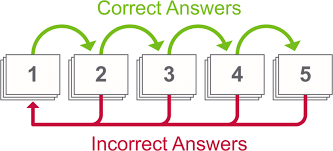
\includegraphics[width=0.5\linewidth]{resx/leitner.png}
    \caption{Visualisation of the Leitner method}
\end{figure}

However the Leitner method is generally executed by a person without the help of a computer. This is because the algorithm is easy and intuitive to perform, so it's most effective for learning flashcards. Since the option for more complicated processing is available, it may be suitable to choose a more effective algorithm. One algorithm which exists is the SuperMemo SM-2 algorithm. This implements two variables for each letter in the Latin alphabet: The `easing factor' \(EF\) abstractly represent the difficulty of a given letter, and the number of repetitions \(n\) is the number of times the letter has been correctly drawn in a row. From this state defined by these two variables, the amount of time between showing a given letter can be calculated as a function of \(n\) using a recurrence relation.

\begin{gather*}
    I(0)=0 \\
    I(1)=1 \\
    I(2)=6 \\
    I(n)=I(n-1)\times EF \\
    I(n)=6\times EF^{(n-2)}
\end{gather*}

To evaluate the `easing factor' of each letter, the letter must be scored on a scale of \(0-5\) depending on the user's confidence. This could be done manually after each round, or by a separate algorithm which uses the accuracy and time of a submission to grade it between \(0-5\). The values in \([0,2]\) represent `forgetting', which in this scenario is equivalent to struggling to write a letter accurately. \\

If the score \(q\) given to the confidence of a letter is in \([0,2]\), then the \(n\) value for that letter is set to the given score. Otherwise, \(n\) is incremented by one since the number of correct repetitions has increased. The `easing factor' is also updated using the score given to the letter.

\begin{equation*}
    \text{EF}'(q) = \min(1.3,\ \text{EF}+f(q))
\end{equation*}
\begin{equation*}
    f(q)=-0.8+0.28q-0.02q^2
\end{equation*}

This means that for any score which is less than a highly accurate recall, the `easing factor' decreases such that the interval for the letter decreases. The function defined by \(f(q)\) has a root at \(q=4\), which is where the interval is not changed.

\newpage
\section{Technical Solution}
\noindent\rule{\textwidth}{0.2pt}

\subsection{Contents}

% go through mark scheme and check where group A,B stuff is i guess

\subsection{Code}

\subsubsection{Server}

\paragraph{connections/accounts.cs}
\begin{minted}{csharp}

\end{minted}
\paragraph{connections/games.cs}
\begin{minted}{csharp}

\end{minted}
\paragraph{connections/queueing.cs}
\begin{minted}{csharp}

\end{minted}
\paragraph{connections/social.cs}
\begin{minted}{csharp}

\end{minted}

\paragraph{databases/Database.cs}
\begin{minted}{csharp}

\end{minted}

\paragraph{games/Accuracy.cs}
\begin{minted}{csharp}

\end{minted}
\paragraph{games/Elimination.cs}
\begin{minted}{csharp}

\end{minted}
\paragraph{games/Game.cs}
\begin{minted}{csharp}

\end{minted}
\paragraph{games/Queueing.cs}
\begin{minted}{csharp}

\end{minted}
\paragraph{games/Versus.cs}
\begin{minted}{csharp}

\end{minted}

\paragraph{neuralNetwork/Backpropagation.cs}
\begin{minted}{csharp}

\end{minted}
\paragraph{neuralNetwork/Data.cs} % data.location
\begin{minted}{csharp}

\end{minted}
\paragraph{neuralNetwork/Network.cs}
\begin{minted}{csharp}

\end{minted}
\paragraph{neuralNetwork/Training.cs}
\begin{minted}{csharp}

\end{minted}

\paragraph{Accounts.cs}
\begin{minted}{csharp}

\end{minted}
\paragraph{logger.cs}
% // delete all references to spectre.console and add some console writes here instead
\begin{minted}{csharp}

\end{minted}
\paragraph{Program.cs}
\begin{minted}{csharp}

\end{minted}

\subsubsection{Client}

\paragraph{components/AlertForm.cs}
\begin{minted}{csharp}

\end{minted}
\paragraph{components/ConfirmForm.cs}
\begin{minted}{csharp}

\end{minted}
\paragraph{components/InputPanel.cs}
\begin{minted}{csharp}

\end{minted}
\paragraph{components/UpdateForm.cs}
\begin{minted}{csharp}

\end{minted}

\paragraph{menus/main.cs}
\begin{minted}{csharp}

\end{minted}
\paragraph{menus/main.Designer.cs}
\begin{minted}{csharp}

\end{minted}
\paragraph{menus/profile.cs}
\begin{minted}{csharp}

\end{minted}
\paragraph{menus/profile.Designer.cs}
\begin{minted}{csharp}

\end{minted}
\paragraph{menus/UXelements.cs}
\begin{minted}{csharp}

\end{minted}

\paragraph{menus/games/Accuracy.cs}
\begin{minted}{csharp}

\end{minted}
\paragraph{menus/games/Elimination.cs}
\begin{minted}{csharp}

\end{minted}
\paragraph{menus/games/Game.cs}
\begin{minted}{csharp}

\end{minted}
\paragraph{menus/games/Versus.cs}
\begin{minted}{csharp}

\end{minted}

\paragraph{hub-connection.cs}
\begin{minted}{csharp}

\end{minted}
\paragraph{localisation.cs}
\begin{minted}{csharp}

\end{minted}
\paragraph{login.cs}
\begin{minted}{csharp}

\end{minted}
\paragraph{login.Designer.cs}
\begin{minted}{csharp}

\end{minted}
\paragraph{Program.cs}
\begin{minted}{csharp}

\end{minted}

\subsection{References}

I have included references to the main documentation used when creating the technical solution. These mainly consist of documentation for the libraries I have used, along with some obscure Windows Forms behaviour. \\

\noindent\href{https://learn.microsoft.com/en-us/dotnet/desktop/winforms/advanced/how-to-create-graphics-objects-for-drawing}{Creating a `Graphics' object to represent the drawing surface of a Panel} \\
\href{https://learn.microsoft.com/en-us/dotnet/desktop/winforms/advanced/how-to-draw-a-line-on-a-windows-form}{Drawing a line between two points on a Panel} \\

\noindent\href{https://learn.microsoft.com/en-us/aspnet/core/tutorials/signalr?view=aspnetcore-10.0&tabs=visual-studio#configure-signalr}{SignalR Documentation} \\
\href{https://github.com/aspnet/SignalR-samples/tree/main/ChatSample/ChatSample}{SignalR configuration example for the server} \\
\href{https://github.com/aspnet/SignalR-samples/tree/main/WindowsFormsSample}{SignalR configuration example for client-side Windows Forms applications} \\
\href{https://learn.microsoft.com/en-us/aspnet/core/signalr/hubcontext?view=aspnetcore-10.0}{Communication outside of a Hub class} \\

\noindent\href{https://grantwinney.com/using-async-await-and-task-to-keep-the-winforms-ui-more-responsive/}{Asynchronous tasks in Windows Forms} \\
\href{https://stackoverflow.com/questions/7609839/accessing-a-forms-control-from-a-separate-thread}{Accessing a Windows Form Control from outside the thread it was created on}

\end{document}
